\chapter{The Calculus of Variations}

Many problems of mathematical physics are connected with the calculus of variations, one of the very central fields of analysis. In this chapter we shall develop certain fundamental concepts of the variational calculus in order to obtain the differential equations of mathematical physics and methods for their solution.

\section{Problems of the Calculus of Variations}

\subsection{Maxima and Minima of Functions}
The calculus of variations originates from a generalization of the elementary theory of maxima and minima. For a better understanding we shall first examine the well-known elementary theory. It is concerned with the problem of finding, for a given continuous function $f(x,y,\ldots)$ in a given closed region $G$, a point $x_0,y_0,\ldots$ in $G$ at which the function $f(x,y,\ldots)$ has a maximum or minimum (extremum) with respect to all points of $G$ in a vicinity of $x_0,y_0,\ldots$. This problem always has a solution, according to the theorem of Weierstrass: \emph{Every function which is continuous in a closed domain $G$ of the variables possesses a largest and a smallest value in the interior or on the boundary of the domain.} If the function $f(x,y,\ldots)$ is differentiable in $G$ and if an extreme value is attained at an interior point $x_0,y_0,\ldots$, then the derivatives of $f(x,y,\ldots)$ with respect to each variable vanish at $x_0,y_0,\ldots$; in other words, the gradient of $f$ is equal to zero. But this necessary condition is in no way sufficient, as can be seen from the existence of points of inflection or saddle points (examples are $f(x)=x^3$ at $x_0=0$; $f(x,y)=xy$ at $x_0=0,y_0=0$). In general, points at which all the derivatives of the function vanish, so that $df=0$, are known as \emph{stationary points}. Stationary points which furnish a maximum or minimum relative to a suitable vicinity are called ``extrema.''

If the variables are not independent but are subject to the restrictions
\[
g_1(x,y,\ldots)=0,\quad g_2(x,y,\ldots)=0,\quad\ldots,\quad g_h(x,y,\ldots)=0,
\]
we obtain necessary conditions for an extremum or stationary point by means of \emph{Lagrange's method of multipliers}. This method consists in the following procedure: In order to find a point in the interior of the domain of the independent variables at which $f(x,y,\ldots)$ has an extremum or is merely stationary, we introduce $h+1$ new parameters, the ``multipliers,'' $\lambda_0,\lambda_1,\ldots,\lambda_h$, and construct the function
\[
F=\lambda_0f+\lambda_1g_1+\lambda_2g_2+\cdots+\lambda_hg_h.
\]
We now determine the quantities $x_0,y_0,\ldots$ and the ratios of $\lambda_0,\lambda_1,\ldots,\lambda_h$ from equations
\begin{equation}\tag{1}
\begin{gathered}
\frac{\partial F}{\partial x}=0,\qquad
\frac{\partial F}{\partial y}=0,\qquad \ldots,\\[0.4em]
\frac{\partial F}{\partial\lambda_1}=g_1=0,\qquad\ldots,\qquad
\frac{\partial F}{\partial\lambda_h}=g_h=0.
\end{gathered}
\end{equation}
the number of which is equal to the number of unknowns. These equations represent the desired conditions for the stationary character of $f(x,y,\ldots)$ or the extremum of $f$ under the given restrictions.

If $\lambda_0\ne0$ we may (and shall) put $\lambda_0=1$ because $F$ is homogeneous in the quantities $\lambda_i$. The Lagrange method is simply a device which, preserving symmetry, avoids explicit elimination of $h$ of the variables from the function $f(x,y,\ldots)$ by means of the subsidiary restrictions.

We now consider a few instructive though elementary examples.

\emph{(a) Of all triangles with given base line and given perimeter the isosceles triangle has the greatest area. Of all triangles with given base line and area the isosceles triangle has the least perimeter.} These statements may easily be verified without calculation by considering the ellipses for which the given base line is the line connecting the two foci. Even this simple example exhibits a characteristic \emph{reciprocity}, which we shall encounter again later (\S12, 2).

\emph{(b) Refraction and Reflection of Light.} According to Fermat's \emph{principle of least time} a ray of light requires less time along its actual path between two points than it would require along any other conceivable (``virtual'') path satisfying the given conditions. From this it follows immediately that light travels in straight lines in any homogeneous medium. If the light ray is required to meet a given curve (mirror) without crossing it, then a simple analysis of the derivative of the light time shows that the path must consist of two straight line-segments making equal angles with the tangent to the given curve at the point where they meet it (\emph{law of reflection}). If, on the other hand, the given curve forms the boundary between two regions in which the velocity of light has the values $c_1$ and $c_2$, respectively, and if the ray is to pass from one region to the other, then it must consist of two straight line-segments which satisfy the well-known \emph{law of refraction (Snell's law)},
\[
\frac{\sin\alpha_1}{\sin\alpha_2}=\frac{c_1}{c_2},
\]
where $\alpha_1$ and $\alpha_2$ are the angles between the normal to the boundary curve and the two line-segments at the point of intersection.

\emph{(c) A Problem of Steiner.} Given three points $A_1,A_2,A_3$ which form an acute triangle, a fourth point $P$ is to be found such that the sum of the distances $PA_1+PA_2+PA_3$ is as small as possible. We consider a circle through $P$ with center at $A_3$; then $P$ must be placed in this circle in such a way that $PA_1+PA_2$ is as small as possible. According to the law of reflection this means that the lines $PA_1$ and $PA_2$ make equal angles with the radius $PA_3$. The same must be true if the indices $1,2,3$ are interchanged; all three angles $A_1PA_2$, $A_2PA_3$, $A_3PA_1$ must, therefore, be equal and equal to $2\pi/3$. Thus the problem is solved.

\emph{(d) The Isoperimetric Problem for Polygons.} Among all polygons which are not self-intersecting and have an even number $2n$ of sides and a given perimeter $2l$ find the one with the greatest area. The desired polygon $\Pi(A_1,A_2,\ldots,A_{2n})$ is the regular $2n$-gon. To prove this we first convince ourselves that $\Pi$ is convex. If $\Pi$ were not convex, a straight line lying entirely outside $\Pi$ could be drawn through two non-adjacent vertices, say $A_k$ and $A_l$; we could then reflect the polygonal sequence $A_kA_{k+1}\cdots A_{l-1}A_l$ in this straight line and obtain a polygon with the same perimeter and with an area greater than that of the original polygon by twice the area of the triangle $A_1A_2A_3$. We may thus confine ourselves to convex polygons. Next we show that all the sides of the polygon are equal in length. For, if the lengths of two successive sides $A_1A_2$ and $A_2A_3$ were different, we could, according to the result of (a), replace the vertex $A_2$ by a vertex $A'_2$ such that $A_1A'_2+A'_2A_3=A_1A_2+A_2A_3$ while the area of the triangle $A_1A'_2A_3$ is greater than that of $A_1A_2A_3$. Thus the area of the polygon with the vertex $A'_2$ is greater than that of the polygon with $A_2$, in contradiction to the hypothesis that $\Pi$ is the maximal polygon. Finally, in order to show that the polygon $\Pi$ can be inscribed in a circle, we divide $\Pi$ into two polygons by means of the diagonal connecting opposite vertices $A_1$ and $A_{n+1}$. The perimeters of these polygons $\Pi_1$ and $\Pi_2$ are evidently equal; their areas are also equal, for if that of $\Pi_1$ were greater than that of $\Pi_2$ we could replace $\Pi_2$ by the reflection of $\Pi_1$ in the diagonal, obtaining a new polygon $\Pi^*$ whose perimeter is still $2l$ but whose area is twice that of $\Pi_1$ and therefore greater than that of $\Pi$. We now show that for every vertex $A_h$ the angle $A_1A_hA_{n+1}$ must be a right angle. For, if this angle were not right for the vertex $A_h$ of $\Pi_1$, we could decompose $\Pi_1$ into the triangle $A_1A_hA_{n+1}$ and two polygons $H_1$ and $H_2$ which join the triangle at the sides $A_1A_h$ and $A_hA_{n+1}$. Consider a right triangle $A'_1A_hA'_{n+1}$ whose sides $A'_1A_h$ and $A_hA'_{n+1}$ are equal to $A_1A_h$ and $A_hA_{n+1}$, respectively. The area of this triangle is greater than that of $A_1A_hA_{n+1}$. If we affix the polygons $H_1$ and $H_2$ to the new triangle at its sides and reflect the resulting polygon in the line $A'_1A'_{n+1}$ we obtain a polygon of perimeter $2l$ and area greater than that of $\Pi$, contrary to hypothesis. Therefore $A_1A_hA_{n+1}$ is a right triangle, and consequently all vertices lie on a circle. This completes the proof of the extremum property of the regular polygon.\footnote{Note that the \emph{existence} of the extremum follows from Weierstrass' theorem. For, if one vertex is at the origin the others are confined to a bounded region, since the total perimeter is given and the area of the polygon is a continuous function of the coordinates of the vertices.}

The preceding treatment, based on a classical idea of Steiner, shows that in individual cases a direct geometrical approach may lead more readily to the result than general analytic procedures.

\emph{(e) Other Examples, Maximum of a Minimum.} We have already encountered other typical examples of stationary values which are neither maxima nor minima but maxima of a minimum or minima of a maximum. For instance, we defined the eigenvalues of quadratic forms as maxima of minima and the Tchebycheff polynomials by a similar property.

\subsection{Functionals}
The calculus of variations likewise originates from the quest for extrema or stationary values. Its object is, however, to find extrema of \emph{functionals} rather than extrema of functions of a finite number of independent variables. By a ``functional'' we mean a quantity or function which depends on the entire course of one or more functions rather than on a number of discrete variables. In other words, the domain of a functional is a set or ``space'' of admissible \emph{functions} rather than a region of a coordinate space. A simple example is the length $L$ of a curve $y=y(x)$ between the values $x=x_0$ and $x=x_1$. This length is given by the integral
\[
L=\int_{x_0}^{x_1}\sqrt{1+y'^2}\,dx;
\]
thus the value of $L$ depends on the course of the ``argument function'' $y(x)$, which may be taken to be an arbitrary continuous function with a piecewise continuous derivative. Such functionals occur throughout analysis and its applications, and many important problems of analysis are concerned with functional dependence of this kind.

Another example is the area of a surface $z=z(x,y)$ lying above the region $G$ in the $xy$-plane. This is given by the integral
\[
\iint_G\sqrt{1+z_x^2+z_y^2}\,dx\,dy\footnote{Throughout this book we shall employ the subscript notation for partial derivatives, i.e. $f_x=\partial f(x,y,\ldots)/\partial x$; $f_{xy}=\partial^2f/\partial x\partial y$, etc.}
\]
and is a functional of the argument function $z(x,y)$.

Other examples of functionals occurred in the previous chapter. Thus for fixed $K(x,y)$ the function
\[
g(x)=\int K(x,y)h(y)\,dy
\]
is a functional of $h(y)$ depending on $x$ as a parameter;\footnote{Often the words ``function of a function'' or ``functional transform'' are used for functionals which themselves depend on variables.} and the integral form
\[
\iint K(x,y)\varphi(x)\varphi(y)\,dx\,dy
\]
is a functional of $\varphi(x)$. In this chapter we shall be concerned principally with functionals which are integrals of known functions of the argument function, its derivatives, and independent variables, such as the arc length of a curve.

A region of definition is needed for a finite number of variables; here we must define the \emph{domain} or ``\emph{space}'' of \emph{admissible functions} from which the argument functions can be selected. This space may, for example, be the set of all functions which are continuous and have piecewise continuous first derivatives (compare the following section).

Although a functional cannot be expressed as a function of a finite number of variables, it may be regarded as a \emph{function of infinitely many variables}. Suppose that the argument functions are expanded in power series or Fourier series; the functional then depends on the expansion coefficients, which constitute the infinitely many variables. Of course the domain of these variables must be restricted so as to conform to the conditions imposed on the argument functions.

\subsection{Typical Problems of the Calculus of Variations}
The calculus of variations is concerned with the problem of determining maxima or minima or, in general, stationary values\footnote{In \S3, 1 the ``stationary value of a functional'' will be defined precisely.} of functionals by seeking that argument function, in the given domain of admissible functions for which the functional assumes the stationary value or extremum in question. Ordinary extremum problems of the differential calculus do not usually involve absolute maxima or minima, but only \emph{an} extremum with respect to values of the function in the vicinity of the extremum point; in analogy, we shall seek here the extremum of the functional only with respect to argument functions in a certain neighborhood of the extremal\footnote{An extremal function is a function which makes a given functional stationary.} argument function. For this purpose it is necessary to define the concept of the \emph{neighborhood of a function} $f(x,y,\ldots)$. If $h$ is a positive quantity, a function $f_1(x,y,\ldots)$ is said to lie in the neighborhood $(h)$ of the function $f(x,y,\ldots)$ if $|f-f_1|<h$ throughout the region of definition.\footnote{For certain problems it is convenient to refine the concept of neighborhood in successive steps. The function $f_1(x,y,\ldots)$ is said to be in the neighborhood of first order $(h)$ of $f(x,y,\ldots)$ if the relations $|f_x-f_{1x}|<h$, $|f_y-f_{1y}|<h$, $\ldots$ are satisfied in addition to $|f-f_1|<h$. More generally, we speak of a neighborhood of order $n+1$ if these inequalities hold for $f_1$ and all its derivatives up to and including the $n$-th order.}

We are now in a position to formulate the \emph{fundamental problem of the calculus of variations}: In a given domain of admissible argument functions, find an argument function (or functions) of a given functional for which the latter is an extremum with respect to all argument functions of the domain lying in a sufficiently small neighborhood $(h)$ of the extremal argument function. If the functional to be made an extremum depends explicitly on variable parameters $x,y,\ldots$ in addition to the argument functions, i.e. if the functional is not a number but a function of these parameters, then we must determine these parameters as well as the argument functions, in order to obtain the extremum. We shall now illustrate the problems of the variational calculus by a number of simple examples.

\emph{(a) Geodesic Curves.} On a given surface, find the shortest curve between two given points. If the surface is given by the parametric representation $x=x(u,v)$, $y=y(u,v)$, $z=z(u,v)$ in rectangular coordinates $x,y,z$, and if we employ the customary notations
\[
e=x_u^2+y_u^2+z_u^2,\qquad
f=x_ux_v+y_uy_v+z_uz_v,\qquad
g=x_v^2+y_v^2+z_v^2,
\]
then the length $L$ of a curve on the surface defined by the equation $v=v(u)$ between $u_0$ and $u_1$ is given by the integral
\[
L=\int_{u_0}^{u_1}\sqrt{e+2fv'+gv'^2}\,du.
\]
The problem is thus to find functions $v(u)$ which yield extrema of this integral.

\emph{(b) Light Rays; Brachistochrone.} According to Fermat's principle (page 165) the path of a light ray in an inhomogeneous two-dimensional medium in which the velocity of light is $c(x,y)$ solves the variational problem
\[
T=\int_{x_0}^{x_1}\frac{\sqrt{1+y'^2}}{c(x,y)}\,dx=\min.
\]
In this problem, as in the previous one, all continuous curves are admissible which have piecewise continuous derivatives and join the given end points of the path. Closely related to the problem of the light ray is the brachistochrone problem, with which Jakob Bernoulli in 1696 gave the initial impetus to the development of the calculus of variations. Two points $A(x_0,0)$ and $B(x_1,y_1)$ with $y_1>0$ are to be connected by a curve along which a frictionless mass point moves in the shortest possible time from $A$ to $B$ under gravity acting in the $y$-direction. The initial velocity of the mass point is zero. After falling a distance $y$ the point has the velocity $\sqrt{2gy}$, according to elementary mechanics, where $g$ is the acceleration due to gravity. It follows that the time of transit is the integral
\begin{equation}\tag{2}
T=\int_{x_0}^{x_1}\sqrt{\frac{1+y'^2}{2gy}}\,dx.
\end{equation}
The class of admissible functions consists of all the positive functions $y(x)$ with continuous second derivatives for which $y(x_0)=0$ and $y(x_1)=y_1$.

\emph{(c) Minimal Surface of Revolution.} Suppose that the curve $y=y(x)\ge0$ is rotated about the $x$-axis. The resulting surface, bounded by planes $x=x_0$ and $x=x_1$, has the area
\[
F=2\pi\int_{x_0}^{x_1}y\sqrt{1+y'^2}\,dx.
\]
The curve $y=y(x)$ which leads to the smallest surface of revolution is thus characterized by the variational problem
\[
\int_{x_0}^{x_1}y\sqrt{1+y'^2}\,dx=\min.
\]

\emph{(d) Isoperimetric Problem.} The original formulation of this problem is: Find a closed curve of given circumference and greatest area. Assuming the curve to be convex and divided into two parts of equal area by the $x$-axis (see subsection 1(d)) we arrive at the following problem: The integral
\[
\int_0^{\xi}y(x)\,dx
\]
is to be made a maximum by a suitable choice of $\xi$ and $y(x)$, while the integral
\[
\int_0^{\xi}\sqrt{1+y'^2}\,dx=l
\]
has a given value. Here $y(x)$ may be any function which is continuous and has a piecewise continuous first derivative in the interval $0\le x\le\xi$ and for which $y(0)=y(\xi)=0$.

An analogous problem may be formulated with the upper limit $\xi$ fixed.

This problem, known as the special isoperimetric problem, may be reduced to a simpler type of variational problem by introducing as the independent variable the arc length
\[
s=\int_0^x\sqrt{1+y'^2}\,dx,
\]
ranging through the interval $0\le s\le l$. Since $ds^2=dx^2+dy^2$, the problem now becomes: Find the function $y(s)$ which maximizes the integral
\[
\int_0^l y\sqrt{1-(dy/ds)^2}\,ds,
\]
where $y(s)$ is a continuous function of $s$ with a piecewise continuous derivative. After determining $y(s)$ we find
\begin{equation}\tag{3}
x(s)=\int_0^s\sqrt{1-\left(\frac{dy}{ds}\right)^2}\,ds
\end{equation}
and thus obtain a parametric representation of the desired curve. (Compare also Hurwitz's solution of the isoperimetric problem, Ch. II, \S10, 1.)

In general, all problems in which one integral expression is to be made an extremum while another has a given value are termed \emph{isoperimetric problems}. An example is given by the \emph{problem of the catenary}: Determine the location of a uniform string of given length with fixed end points under the influence of gravity. Suppose that gravity acts in the negative $y$-direction. Since the equilibrium position demands that the center of gravity be as low as possible, we arrive at the following variational problem: Find the function $y(x)$ for which
\[
\int_{x_0}^{x_1}y\sqrt{1+y'^2}\,dx
\]
is as small as possible while
\[
l=\int_{x_0}^{x_1}\sqrt{1+y'^2}\,dx
\]
has a given value, and the boundary values $y(x_0)=y_0$, $y(x_1)=y_1$ are given.

Another problem is to solve
\[
\int_{x_0}^{x_1}(y'')^2\,dx=\min.
\]
with the subsidiary condition
\[
\int_{x_0}^{x_1}y^2\,dx=1,
\]
where the function $y(x)$ is to vanish at the end points of the interval and is to be continuous everywhere along with its derivatives up to the second order. Another very important isoperimetric problem is: Find a function $u$ of $x$ and $y$, continuous along with its first derivatives in the region $G$, which satisfies $\iint_Gu^2\,dx\,dy=1$ and for which
\begin{equation}\tag{4}
\iint_G(u_x^2+u_y^2)\,dx\,dy+\int_{\Gamma}\sigma u^2\,ds
\end{equation}
is as small as possible\footnote{Cf. \S3, 2.} (here $\Gamma$ is the boundary of the region $G$ and $\sigma$ is a fixed function of the arc length $s$ of $\Gamma$). The minimum problem of Chapter III for the eigenfunctions of a symmetric kernel is another example of an isoperimetric problem.

It goes without saying that in all these problems the space of admissible argument functions must be specified by continuity conditions such that all the functionals occurring in the problem are meaningful.

\subsection{Characteristic Difficulties of the Calculus of Variations}
In the theory of ordinary maxima and minima the existence of a solution is ensured by the fundamental theorem of Weierstrass. In contrast, the characteristic difficulty of the calculus of variations is that problems which can be meaningfully formulated may not have solutions---because it is not in general possible to choose the domain of admissible functions as a ``compact set'' in which a principle of points of accumulation is valid. A simple geometric example is the following: Two points on the $x$-axis are to be connected by the shortest possible line of continuous curvature which is perpendicular to the $x$-axis at the end points. This problem has no solution. For, the length of such a line is always greater than that of the straight line connecting the two points, but it may approximate this length as closely as desired. Thus there exists a greatest lower bound but no minimum for admissible curves.

Another example of an insoluble variational problem is the following: Minimize the integral
\begin{equation}\tag{5}
\int_{-1}^{1}x^4y'^2\,dx
\end{equation}
by means of a continuous function $y(x)$ which has a piecewise continuous derivative and for which $y(-1)=-1$, $y(1)=1$. It is easily seen that the integral can be made arbitrarily small by suitable functions (i.e. $y=-1$ for $x<-\epsilon$, $y=x/\epsilon$ for $|x|\le\epsilon$, $y=1$ for $x>\epsilon$), but does not vanish for any admissible function.

Thus, \emph{in the calculus of variations the existence of an extremum in a particular problem cannot be taken for granted}. A special existence proof is needed for the solution of each problem or class of problems. As we shall see later, this fact gives rise to essential difficulties in many of the problems of the calculus of variations. However, in this chapter we shall deal primarily with the formulation of \emph{necessary conditions} for the attainment of an extremum, while the question whether an extremum is actually attained when the conditions are satisfied may be left open.

Before formulating these necessary conditions we shall consider possible methods for the direct solution of variational problems.

\section{Direct Solution}\footnote{Direct methods of the calculus of variations will be treated more fully in the second volume.}

Direct and complete solutions of variational problems can sometimes be obtained by a general procedure consisting of two steps: first one formulates a suitable approximate ordinary extremum problem in which only a finite number $n$ of parameters is to be determined and then one passes to the limit $n\to\infty$ in the solution of the approximate problem.

\subsection{The Isoperimetric Problem}
One example is the isoperimetric problem of \S1, 3(d): find a closed curve $K$ with perimeter $2l$ and maximum area; the curve is to be piecewise smooth, i.e. it is to have a continuous tangent except at a finite number of corners. If we assume that the solution is given by the curve $K$ we may conclude that $K$ is a circle. For, just as in \S1, 1(d), it may be proved that $K$ is convex and that every secant $AB$ which divides $K$ into two parts with equal circumference also divides it into two parts of equal area; furthermore, for every point $P$ on $K$ the angle $APB$ must be a right angle, since otherwise, by the construction of \S1, 1(d), one could obtain a curve $K'$ with the same perimeter but greater area. But this argument is based on the tacit assumption that the problem actually possesses a solution, and this assumption requires proof; therefore we shall solve the problem by a different method which furnishes the necessary existence proof at the same time. We consider the set of values of the areas of admissible curves. Since these numbers all lie below the bound $l^2\pi$ (the curve can certainly be placed inside a circle of radius $l$), this set of numbers has, by the elementary rules of analysis, a least upper bound $M$, above which there is no number of the set, but such that numbers of the set occur in any neighborhood $(\epsilon)$ of $M$ for arbitrarily small $\epsilon$. In other words, there exists a ``maximizing sequence'' of admissible curves $K_1,K_2,\ldots$ such that the area $F_n$ of $K_n$ converges to $M$ with increasing $n$. Now every curve $K_n$ can be approximated as exactly as desired by an inscribed polygon $\Pi_n$ with sufficiently many sides such that area and perimeter of $\Pi_n$ differ arbitrarily little from those of $K_n$. We may, without destroying its approximating character, dilate each polygon in such a way that its perimeter becomes exactly equal to $2l$. Thus the maximizing sequence $K_1,K_2,\ldots$ may be replaced by a maximizing sequence of polygons $\Pi'_1,\Pi'_2,\ldots$. The number of sides of these polygons may be assumed to be even, since a $(2m-1)$-gon may be regarded as a $2m$-gon with two adjacent sides forming part of one same straight line. We know from \S1, 1(d) that of all $2m$-gons of perimeter $2l$ the regular $2m$-gon has the greatest area. We therefore obtain an even better maximizing sequence of our problem by replacing each polygon $\Pi'_n$ by a corresponding regular polygon. But as the number of sides increases these polygons converge to the circle of perimeter $2l$, and since the areas of the polygons converge to $M$ the circle has the area $M$ and is actually the solution of our variational problem.

\subsection{The Rayleigh-Ritz Method. Minimizing Sequences}
The above considerations are based on the following general idea: We consider any variational problem of the form $D[\varphi]=\min.$, where the functional $D[\varphi]$ is an integral of a given expression containing the function $\varphi$ and its derivatives up to the $k$-th order, and where the region of integration and the domain of admissible functions $\varphi$ are given. It does not matter whether $D[\varphi]$ is a simple or a multiple integral. We assume that the set of values of $D[\varphi]$ for the admissible argument functions $\varphi$ possesses a greatest lower bound $d$ (whether $d$ is a minimum which is actually attained for a function $\varphi=u$ remains an open question). Then there exist sequences $\varphi_1,\varphi_2,\ldots$ of admissible functions such that $\lim_{n\to\infty}D[\varphi_n]=d$, while the relation $D[\varphi]\ge d$ holds for every admissible function $\varphi$. Such sequences of functions will be called \emph{minimizing sequences} of the variational problem. \emph{A direct solution of the variational problem always consists in the construction of minimizing sequences and the attempt to secure the solution by a limiting process based on this sequence.}

The method which W. Ritz\footnote{W. Ritz, \emph{"Uber eine neue Methode zur L\"osung gewisser Variationsprobleme der mathematischen Physik}, Journ. f. d. reine u. angew. Math., Vol. 135, 1909, pp. 1--61; Gesammelte Werke, pp. 192--250, Gauthier-Villars, Paris, 1911. Even before Ritz, similar ideas were successfully employed by Lord Rayleigh.} used with great success, especially for numerical solutions, consists in the following steps: We start with a fixed complete system of ``coordinate'' functions $\omega_1,\omega_2,\ldots$, defined in the region of integration, which has the property\footnote{The question of the existence of such functions will be discussed more fully in the second volume.} that all linear combinations $\varphi_n=c_1\omega_1+c_2\omega_2+\cdots+c_n\omega_n$ of a finite number of the functions are admissible comparison functions for the problem, and such that for every admissible function $\varphi$ there is a suitable combination $\varphi_n$ of this kind for which $D[\varphi]$ differs arbitrarily little from $D[\varphi_n]$. Then there exist minimizing sequences $\varphi_1,\varphi_2,\ldots$ in which $\varphi_n$ is a linear combination $c_1\omega_1+c_2\omega_2+\cdots+c_n\omega_n$ of the functions $\omega_1,\omega_2,\ldots,\omega_n$. We therefore obtain an even better minimizing sequence if for every $n$ we determine the function $\varphi_n$, i.e. the parameters $c_1,c_2,\ldots,c_n$, by the requirement that $D[\varphi_n]=d_n$ be a minimum. This requirement represents an ordinary minimum problem for $D[\varphi_n]$ as a function of the $n$ parameters $c_1,c_2,\ldots,c_n$ and can always be fulfilled, according to Weierstrass's theorem (provided $D[\varphi_n]$ is a continuously differentiable function of $c_1,c_2,\ldots,c_n$; we shall assume here that this is the case). The values $c_i$ are determined by the $n$ simultaneous equations $\partial D[\varphi_n]/\partial c_i=0$ $(i=1,2,\ldots,n)$. We may now expect the resulting minimizing sequence to converge to the desired solution. Unfortunately things are not so simple, as we shall see in \S4. In general we can only state that the values $D[\varphi_n]=d_n$ obtained in this way converge to the desired greatest lower bound or minimum. Whether the minimizing sequence itself converges to the solution is a difficult theoretical question which has to be investigated separately. We shall return to this question on several subsequent occasions.

In some cases this method may prove useful for numerical calculations even though its convergence is unproved. Its success in any particular case will depend on the proper choice of \emph{coordinate functions} $\omega_i$. The method will be illustrated by examples in the next subsection.

\subsection{Other Direct Methods. Method of Finite Differences. Infinitely Many Variables}
One can often obtain minimizing sequences by extending the domain of admissible functions, for example by admitting not only continuously differentiable functions, but also continuous functions with piecewise continuous derivatives. We shall consider the problem of the minimum of a simple integral of the form
\[
D[y]=\int_{x_0}^{x_1}F(x,y,y')\,dx.
\]
If $y=\varphi_1(x)$, $y=\varphi_2(x),\ldots$ is a minimizing sequence, and if $F(x,y,y')$ satisfies the necessary continuity requirements, then the curve given by $y=\varphi_n(x)$ can certainly be approximated by a polygonal arc $y=p_n(x)$ in such a way that the integral $D[\varphi_n]$ differs arbitrarily little from $D[p_n]$. It is therefore possible to construct minimizing sequences consisting of piecewise linear functions, for which the difference quotient and the differential quotient are identical in each subinterval. Thus if we divide the interval of integration by $m$ points into equal parts of length $\Delta x$, and if we confine ourselves to functions which are linear in each subinterval, the variational problem goes over into, or may be approximately replaced by, the ordinary minimum problem
\[
\sum_{i=0}^{m}F\!\left(x_i,y_i,\frac{y_{i+1}-y_i}{\Delta x}\right)\Delta x=\min.
\]
for the values $y_0,y_1,\ldots,y_{m+1}$ of the function at the ends of the subintervals. The resulting functions for $m=0,1,2,\ldots$ once again form a minimizing sequence.\footnote{The method described here is essentially the method which led Euler to the ``Euler differential equations'' in his work: \emph{Methodus inveniendi lineas curvas maximi minimive proprietate gaudentes}, M. Bousquet, Lausanne and Geneva, 1744.}

This method may be regarded as a special case of the Ritz method, with suitable piecewise linear coordinate functions.

Under what circumstances the solution of the finite difference problem converges to the solution of the minimum problem will be discussed in the second volume.

It is possible to proceed in a similar manner when the integrand contains derivatives of higher order, say the second. The second differential quotients will then be replaced in the approximating problem by the second difference quotients $(y_{i+2}-2y_{i+1}+y_i)/(\Delta x)^2$.

Our variational problems may also be regarded as problems in the theory of functions of infinitely many variables. For example, in Hurwitz's solution of the isoperimetric problem (Ch. II, p. 97) the variables in question were the Fourier coefficients and the analytic expression for $L^2-4\pi F$ exhibits the solution. The Ritz method also admits of this interpretation if we may assume the function to be developed in a Fourier series $c_1\omega_1+c_2\omega_2+\cdots$ and regard the method as a prescription for obtaining the infinitely many coefficients $c_1,c_2,\ldots$. The difficult question of convergence would have to be investigated separately.

We shall now illustrate these general considerations by some examples.

\emph{(a) The integral}
\begin{equation}\tag{6}
D[\varphi]=\iint_R(\varphi_x^2+\varphi_y^2)\,dx\,dy,
\end{equation}
which extends over the rectangle $R$ given by $0\le x\le a$, $0\le y\le b$, is to be minimized; here the admissible comparison functions are all piecewise smooth\footnote{See the definition given in Ch. II, p. 48.} in $R$, vanish on its boundary, and satisfy the subsidiary condition
\begin{equation}\tag{7}
H[\varphi]=\iint_R\varphi^2\,dx\,dy=1.
\end{equation}
We suppose that the function $\varphi$ is expanded in a Fourier series
\[
\varphi=\sum_{m,n=1}^{\infty}c_{mn}\sin\frac{m\pi x}{a}\sin\frac{n\pi y}{b};
\]
this is certainly possible according to Chapter II. The problem is to determine the infinitely many parameters $c_{mn}$ from the minimum requirement. Since the functions $\varphi_x$ and $\varphi_y$ are piecewise continuous we may apply the completeness relation of the trigonometric functions to these functions with the expansion coefficients $(\pi m/a)c_{mn}$, $(\pi n/b)c_{mn}$, obtaining for the two integrals the expressions
\begin{equation}\tag{8}
D=\pi^2\frac{ab}{4}\sum_{m,n=1}^{\infty}c_{mn}^2\left(\frac{m^2}{a^2}+\frac{n^2}{b^2}\right);\qquad
H=\frac{ab}{4}\sum_{m,n=1}^{\infty}c_{mn}^2
\end{equation}
in the parameters $c_{mn}$. Because of the condition $H=1$ it is now evident that the solution of the problem is given by $c_{mn}=0$ except for the coefficient $c_{11}$, which must equal $2/\sqrt{ab}$. Thus our variational problem is solved by the function
\[
u=\frac{2}{\sqrt{ab}}\sin\frac{\pi x}{a}\sin\frac{\pi y}{b},
\]
and the value of the minimum is
\[
d=\pi^2\left(\frac{1}{a^2}+\frac{1}{b^2}\right).
\]
This may be expressed by relation
\begin{equation}\tag{9}
D[\varphi]\ge\pi^2\left(\frac{1}{a^2}+\frac{1}{b^2}\right)H[\varphi]
\end{equation}
for every piecewise smooth function vanishing on the boundary of the rectangle, because this relation is equivalent to $D[\psi]\ge d$ for the normalized function $\psi=\varphi/\sqrt{H[\varphi]}$.

\emph{(b) Dirichlet's Problem\footnote{This nomenclature has become customary since Riemann's time even though it does not correspond to the historical facts.} for the Circle.} The integral
\[
D[\varphi]=\iint_K(\varphi_x^2+\varphi_y^2)\,dx\,dy,
\]
extended over the circle $K$ ($x^2+y^2\le1$) in the $x,y$-plane, is to be made a minimum if the admissible comparison functions are smooth in $K$ and assume given boundary values on the boundary of $K$. We introduce polar coordinates $r,\theta$ in $K$, transforming the integral into
\[
D[\varphi]=\int_0^{2\pi}\int_0^1\left(\varphi_r^2+\frac{1}{r^2}\varphi_\theta^2\right)r\,dr\,d\theta.
\]
The boundary values may now be defined by a Fourier series
\[
f(\theta)=\frac12 a_0+\sum_{n=1}^{\infty}(a_n\cos n\theta+b_n\sin n\theta).
\]
Suppose further that this boundary function $f$ has a smooth derivative; according to Ch. II, \S5, 3, this means that $n^2|a_n|$ and $n^2|b_n|$ are bounded. We may now assume the function $\varphi$ written in the form
\[
\varphi=\frac12 f_0(r)+\sum_{n=1}^{\infty}[f_n(r)\cos n\theta+g_n(r)\sin n\theta],
\]
where $f_n(r),g_n(r)$ must satisfy the relations $f_n(1)=a_n$, $g_n(1)=b_n$. Because of the completeness relation for the trigonometric functions we obtain the equation
\[
\begin{aligned}
D[\varphi]={}&\pi\int_0^1[f_0'(r)]^2r\,dr\\
&+\pi\sum_{n=1}^{\infty}\int_0^1\left[f_n'^2(r)+\frac{n^2}{r^2}f_n^2(r)\right]r\,dr\\
&+\pi\sum_{n=1}^{\infty}\int_0^1\left[g_n'^2(r)+\frac{n^2}{r^2}g_n^2(r)\right]r\,dr.
\end{aligned}
\]
Thus in order to solve the original minimum problem we treat the series of minimum problems
\[
\int_0^1\left(f_n'^2+\frac{n^2}{r^2}f_n^2\right)r\,dr=\min.,
\qquad
\int_0^1\left(g_n'^2+\frac{n^2}{r^2}g_n^2\right)r\,dr=\min.
\qquad (n=0,1,2,\ldots),
\]
in which $f_n$ and $g_n$ are smooth functions that take on the values $a_n$ and $b_n$, respectively, at $r=1$. In view of Weierstrass's approximation theorem the functions $1,r,r^2,\ldots$ certainly satisfy the conditions for the coordinate functions of the Ritz method for these minimum problems. Let us take for $f_n$ (or $g_n$) a polynomial $c_{n,0}+c_{n,1}r+\cdots+c_{n,m}r^m$ with $m\ge n$ and with $c_{n,0}+c_{n,1}+\cdots+c_{n,m}=a_n$ (or $b_n$). The reader may easily verify that the solutions, independent of $m$, are $f_n=a_nr^n$ (or $g_n=b_nr^n$). Thus all the functions of the resulting minimizing sequence are equal to each other, and therefore equal to the solution of the variational problem.

The solution $f_n$ or $g_n$ of the variational problem may also be found directly, without employing the Ritz procedure, in the following way: For $n=0$ we have to minimize $\int_0^1 f_0'^2r\,dr$; this is evidently accomplished with $f_0'=0$, $f_0=\mathrm{const.}=a_0$. For $n>0$ we must have $f_n(0)=g_n(0)=0$; otherwise the second part of the integral would be infinite, since $f_n$ is differentiable and may therefore be written in the form $f_n(0)+rh_n(r)$ with a continuous function $h_n(r)$. We now write the first integral in the form
\[
\int_0^1\left(f_n'-\frac{n}{r}f_n\right)^2r\,dr+2n\int_0^1f_nf_n'\,dr
=\int_0^1\left(f_n'-\frac{n}{r}f_n\right)^2r\,dr+n f_n^2(1).
\]
The value of $f_n(1)=a_n$ is fixed, and we see immediately that we obtain a minimum value, namely $n f_n^2(1)=na_n^2$, if we set $f_n'-n f_n/r=0$, obtaining $f_n=c_nr^n$; since $f_n(1)=a_n$ we have $c_n=a_n$ or $f_n=a_nr^n$. Corresponding results are obtained for $g_n(r)$. Thus the solution of the original minimum problem is
\begin{equation}\tag{10}
u(r,\theta)=\frac12a_0+\sum_{n=1}^{\infty}r^n(a_n\cos n\theta+b_n\sin n\theta)
\end{equation}
and the minimum value is
\[
\pi\sum_{n=1}^{\infty}n(a_n^2+b_n^2).
\]
It should be emphasized that the minimum problem solved here may cease to be meaningful if less stringent assumptions are made
concerning the boundary function, for example if continuity alone is required. Thus, if we take the continuous boundary function defined by the uniformly convergent series
\[
\rho(\theta)=\sum_{n=1}^{\infty}\frac{1}{n^2}\cos(n!\theta),
\]
the sum
\[
\pi\sum_{m=1}^{\infty}m a_m^2
=\pi\sum_{n=1}^{\infty}\frac{n!}{n^4}
\]
is infinite. In this case it can easily be shown that there exists no admissible comparison function with finite $D[\varphi]$.

\emph{(c)} Let $g(x,y)$ be a smooth function in the rectangle $R$ defined by $0\le x\le a$, $0\le y\le b$. We seek a function $\varphi$, continuous in the rectangle along with its first derivatives and vanishing on the boundary, which minimizes the integral
\begin{equation}\tag{11}
J[\varphi]=\iint_R(\varphi_x^2+\varphi_y^2-2\varphi g)\,dx\,dy.
\end{equation}
In the interior of $R$, let us write
\[
g(x,y)=\sum_{m,n=1}^{\infty}a_{mn}\sin m\frac{\pi x}{a}\sin n\frac{\pi y}{b}
\]
and
\[
\varphi=\sum_{m,n=1}^{\infty}c_{mn}\sin m\frac{\pi x}{a}\sin n\frac{\pi y}{b},
\]
where the parameters $c_{mn}$ are to be determined. Because of the completeness relation for the trigonometric functions the variational problem then goes over into the problem of determining the quantities $c_{mn}$ such that
\[
\frac{4}{ab}J[\varphi]
=\pi^2\sum_{m,n=1}^{\infty}\left(\frac{m^2}{a^2}+\frac{n^2}{b^2}\right)c_{mn}^2
-2\sum_{m,n=1}^{\infty}a_{mn}c_{mn}
\]
becomes as small as possible. We see immediately that the minimum is furnished by
\[
c_{mn}=\frac{a_{mn}}{\pi^2(m^2/a^2+n^2/b^2)},
\]
\begin{equation}\tag{12}
u(x,y)=\frac{1}{\pi^2}\sum_{m,n=1}^{\infty}\frac{a_{mn}}{m^2/a^2+n^2/b^2}\sin m\frac{\pi x}{a}\sin n\frac{\pi y}{b}.
\end{equation}
This function does indeed satisfy all requirements, since the series, as well as the series obtained by term-by-term differentiation, converges uniformly. To see this we note that the absolutely convergent series
\[
\sum\frac{|a_{mn}|}{m^2/a^2+n^2/b^2},\qquad
\sum\frac{m|a_{mn}|}{m^2/a^2+n^2/b^2},\qquad
\sum\frac{n|a_{mn}|}{m^2/a^2+n^2/b^2}
\]
represent majorants. We shall see subsequently (page 192) that the function $u$ satisfies the differential equation $u_{xx}+u_{yy}=-g(x,y)$;\ctnote{此处原文写作 $u_{xx}+u_{yy}=g(x,y)$。但由 (11) 的泛函 $J[\varphi]=\iint(\varphi_x^2+\varphi_y^2-2\varphi g)\,dx\,dy$ 的 Euler 方程可得 $\Delta u=-g$；同样，由 (12) 中正弦级数逐项求二阶导数，也得到 $u_{xx}+u_{yy}=-g$。故正文改正符号。} compare examples (a) and (b).

\subsection{General Remarks on Direct Methods of the Calculus of Variations}
We have already noted that the main difficulty in justifying the direct methods of the calculus of variations is that minimizing sequences do not necessarily converge to a limit function, even if the existence of a solution is not in question.

A simple example is given by the variational problem of minimal surfaces, in which the integral
\[
\iint_G\sqrt{1+z_x^2+z_y^2}\,dx\,dy
\]
is to be minimized; here we admit all surfaces $z=z(x,y)$ with piecewise continuous derivatives which pass through a given space curve whose projection is the boundary of $G$. If, in particular, we take for this curve a curve in the $x,y$-plane, for example a circle of unit area, the minimum is given by the function $z=0$, i.e. by the $x,y$-plane itself. Every sequence of surfaces which passes through the periphery of the circle and the areas of which converge to $1$ is a minimizing sequence. Now we may at once construct admissible comparison surfaces whose areas are arbitrarily close to $1$ and for which $z(x,y)$ is arbitrarily large at isolated points. For example, consider a circular cone of height $1$ and base radius $\epsilon$ placed perpendicularly on the plane $z=0$. We now take as a comparison surface the surface consisting of this cone and of the portion of the original circle outside the base of the cone. A minimizing sequence of such surfaces does not, for $\epsilon\to0$, converge to the solution. It is even possible, as is easily seen, to construct minimizing sequences in which the points of divergence are everywhere dense in the circle.

Another example is given by the Dirichlet problem of minimizing the integral
\[
D[\varphi]=\iint_G(\varphi_x^2+\varphi_y^2)\,dx\,dy
\]
if we admit for comparison all functions continuous and piecewise smooth in $G$ which vanish on the boundary. Evidently the unique solution of the problem is $\varphi=0$, since every other admissible function leads to a positive value of the integral. Introducing polar coordinates $r,\theta$ about an arbitrary point $P$ of $G$, we write the integral in the form
\[
\iint_G(\varphi_r^2+\varphi_\theta^2/r^2)r\,dr\,d\theta.
\]
We now consider a circle $r\le a$ about $P$, lying entirely in the interior of $G$, with radius $a<1$. Let us set $\varphi=0$ outside this circle, $\varphi=\log(r/a)/\log a$ in the circular ring between $r=a$ and $r=a^2$, and $\varphi=\log a/\log a=1$ in the circle $r\le a^2$. By definition, $\varphi$ is an admissible comparison function; therefore the integral is equal to
\[
\frac{2\pi}{(\log a)^2}\int_{a^2}^{a}\frac{1}{r^2}r\,dr
=-\frac{2\pi}{\log a}.
\]
If we now let $a$ assume a sequence of values $a_1,a_2,\ldots$ which tend to zero and consider the corresponding functions $\varphi_1,\varphi_2,\ldots$, we see that $D[\varphi_n]$ converges to zero; thus these functions form a minimizing sequence of the problem. But at the point $P$ all the functions have the value $1$ and therefore do not converge toward the solution $\varphi=0$ of the problem.

In the case of the variational problem $\int_0^1y'^2\,dx=\min.$, where $y(x)$ is a continuous piecewise smooth function of $x$ vanishing at the end points, all minimizing sequences must indeed converge to the function $y=0$, as is easily seen. But the derivatives of the functions of the minimizing sequence do not necessarily converge to zero, as is shown by the example of the sequence $y_n=x$ for $x<\epsilon_n$, $y_n=2\epsilon_n-x$ for $\epsilon_n\le x\le2\epsilon_n$, $y_n=0$ for $x>2\epsilon_n$ ($\lim_{n\to\infty}\epsilon_n=0$).

In Volume II we shall see how these difficulties may be overcome; indeed, the direct methods of the variational calculus have led to important developments in analysis.

The following sections deal with classical ``indirect'' methods based on the reduction of variational problems to differential equations. These methods, which have been emphasized by mathematicians since Euler and Lagrange, attack minimum problems by means of a general variational formalism which in itself has become an important tool of analysis.

\section{The Euler Equations}
The differential equations of a variational problem, first derived by Euler, represent necessary but by no means always sufficient conditions which a function must satisfy if it is to furnish the extremum of a given integral. We obtain these Euler equations by reducing the variational problem to a problem in the differential calculus. Once and for all we assume that all functions and their derivatives which occur explicitly in the problems are continuous unless the contrary is explicitly stated.

\subsection{``Simplest Problem'' of the Variational Calculus}
Let us first consider the simplest problem of the calculus of variations, namely that of determining the minimum of the integral
\begin{equation}\tag{13}
J[y]=\int_{x_0}^{x_1}F(x,y,y')\,dx,
\end{equation}
where the values $x_0$, $x_1$, $y(x_0)$, $y(x_1)$ are given. The function $F$ is to be twice continuously differentiable with respect to its three arguments $x,y,y'$. The second derivative $y''$ of the function $y$ is also assumed continuous. Suppose $y=y(x)=f(x)$ is the desired extremal function yielding the minimum, i.e. suppose that, in a sufficiently small neighborhood $(h)$ of the function $f(x)$, the integral $J[y]$ is smallest when $y=f(x)$. Now consider a function $\eta(x)$ which is defined in the interval $x_0\le x\le x_1$, possesses a continuous second derivative, and vanishes at the end points, but is otherwise arbitrary. We construct the function $\bar y=y+\epsilon\eta(x)=y+\delta y$, where $\epsilon$ is a parameter. The quantity $\delta y=\epsilon\eta(x)$ is known as the variation of the function $y=f(x)$. If the parameter $\epsilon$ has a sufficiently small absolute value all the varied functions $\bar y$ lie in an arbitrarily small neighborhood of the extremal function $y=f(x)$. Therefore the integral $J[\bar y]=J[y+\epsilon\eta]$, which may be regarded as a function $\Phi(\epsilon)$ of $\epsilon$, must have a minimum at $\epsilon=0$ relative to all values of $\epsilon$ in a sufficiently small neighborhood of $0$, and therefore $\Phi'(0)=0$. Now if we differentiate the integral
\[
\Phi(\epsilon)=\int_{x_0}^{x_1}F(x,y+\epsilon\eta,y'+\epsilon\eta')\,dx
\]
with respect to $\epsilon$ under the integral sign (this is permissible) we obtain as a necessary condition the equation
\[
\Phi'(0)=\int_{x_0}^{x_1}(F_y\eta+F_{y'}\eta')\,dx=0,
\]
which must hold for all functions $\eta(x)$ which satisfy the above requirements. We transform the second part of the integral by partial integration, noting that $\eta(x_0)=\eta(x_1)=0$, and obtain the equation
\[
\int_{x_0}^{x_1}\eta\left(F_y-\frac{d}{dx}F_{y'}\right)dx=0,
\]
valid for every one of our functions $\eta$.

This equation immediately leads to the desired differential equation in virtue of the following \emph{fundamental lemma of the calculus of variations}: If the relation
\[
\int_{x_0}^{x_1}\eta(x)\varphi(x)\,dx=0,
\]
with $\varphi(x)$ a continuous function of $x$, holds for all functions $\eta(x)$ which vanish on the boundary and are continuous together with their first two derivatives, it follows that $\varphi(x)=0$ identically. This lemma, which holds equally well for multiple integrals, is easily proved indirectly. Let us suppose that $\varphi(x)$ is different from zero, say positive, at $x=\xi$. Then there must exist a neighborhood $G$, given by $\xi_0<x<\xi_1$, in which $\varphi(x)$ is positive. We take the function $\eta(x)=(x-\xi_0)^4(x-\xi_1)^4$ in $G$ and $\eta(x)=0$ outside this interval. Then we have $\int_{x_0}^{x_1}\eta\varphi\,dx>0$ in contradiction to the hypothesis. The assertion $\varphi=0$ remains valid if we require that the first $k$ derivatives of the function $\eta$ be continuous; in this case we simply set $\eta=(x-\xi_0)^{2l}(x-\xi_1)^{2l}$ with $2l>k$.

From the fundamental lemma it follows immediately that the function $dF_{y'}/dx-F_y$, which we shall henceforth denote by $-[F]_y$, vanishes identically in $x$, i.e. that the function $y(x)$ satisfies the differential equation
\begin{equation}\tag{14}
-[F]_y=\frac{d}{dx}F_{y'}-F_y=0
\end{equation}
or, written out in detail,
\begin{equation}\tag{14'}
y''F_{y'y'}+y'F_{y'y}+F_{y'x}-F_y=0.
\end{equation}
This is the \emph{fundamental differential equation of Euler}, which occurs time and again throughout analysis and its applications. \emph{Its validity is a necessary condition for the existence of an extremum.} It is a differential equation of the second order, in the general solution of which there occur two arbitrary constants, the number generally required in order to satisfy the boundary conditions. We now define: every solution of Euler's differential equation is an \emph{extremal}\footnote{Cf. definition in footnote 2 on page 169.} of the minimum problem. The differential expression $[F]_y$ is called the \emph{variational derivative} of $F$ with respect to $y$. Its role here is analogous to that of the differential quotient or of the gradient in ordinary minimum problems.

If, as is customary in the theory of differential equations, we want to solve the Euler differential equation for the highest derivative, we have to postulate
\[
F_{y'y'}\ne0.
\]
This inequality is known as the \emph{Legendre condition}; it is of great importance in the problem of investigating whether an extremal actually gives an extremum (compare also \S6, pages 214--216).

The essential idea in the above considerations is to imbed the extremal $y(x)$ in a family of functions $y(x)+\epsilon\eta(x)$ with the parameter $\epsilon$. The fact that this parameter occurs linearly is not important. It is often convenient to imbed the function in a more general family of functions $y(x,\epsilon)$; the above considerations remain valid if we set
\[
\eta(x)=\left.\frac{\partial}{\partial\epsilon}y(x,\epsilon)\right|_{\epsilon=0}.
\]

We now introduce a useful terminology. We called the function $\epsilon\eta=\delta y$ the variation of $y(x)$; similarly the expression
\begin{align}\tag{15}
\delta J
&=\epsilon\Phi'(0)=\epsilon\int_{x_0}^{x_1}(\eta F_y+\eta'F_{y'})\,dx\\
&=\epsilon\int_{x_0}^{x_1}\left(F_y-\frac{d}{dx}F_{y'}\right)\eta\,dx
 +\epsilon F_{y'}\eta\big|^{x=x_1}-\epsilon F_{y'}\eta\big|^{x=x_0}\\
&=\int_{x_0}^{x_1}[F]_y\,\delta y\,dx+F_{y'}\,\delta y\big|_{x_0}^{x_1},
\end{align}
even if $\eta$ does not vanish at the boundary, is called the variation or more precisely the \emph{first variation} of the integral $J$. This is analogous to the notation of the differential calculus, where the expression $\epsilon f'(x)=df$ with an arbitrary parameter $\epsilon$ is called the differential of the function $f(x)$. Thus \emph{a necessary condition for a minimum is the vanishing of the first variation for all $y+\delta y$ which satisfy the boundary conditions}.

In general, functions or, geometrically speaking, curves for which $\delta J$ vanishes, i.e. extremals, are sometimes called \emph{stationary functions or curves}. This terminology indicates that we may be dealing with circumstances other than actual extrema, just as in the corresponding problems of the differential calculus. There are, in fact, many cases in which one is primarily interested in the vanishing of the variation rather than in the question of an extremum. Problems in which one is merely interested in obtaining stationary values are likewise called \emph{variational problems}.

The examples considered above (pages 170--173) lead to the following variational derivatives:
\begin{align*}
\text{(a)}\quad &F=\sqrt{e+2fv'+gv'^2},\\
&\frac{d}{du}\frac{f+gv'}{\sqrt{e+2fv'+gv'^2}}
-\frac{e_v+2f_vv'+g_vv'^2}{2\sqrt{e+2fv'+gv'^2}}=0;\\[0.5em]
\text{(b)}\quad &F=\frac{\sqrt{1+y'^2}}{\varphi(x,y)}=\psi(x,y)\sqrt{1+y'^2},\\
&\psi y''=(\psi_y-\psi_x y')(1+y'^2);\\[0.5em]
\text{(c)}\quad &F=y\sqrt{1+y'^2},\qquad yy''=1+y'^2\quad\text{(a special case of (b));}\\[0.5em]
\text{(d)}\quad &F=y\sqrt{1-y'^2},\qquad yy''=y'^2-1.
\end{align*}
We shall return to the integration of these differential equations in \S4.

\subsection{Several Unknown Functions}
A straightforward generalization of the problem discussed in subsection 1 is the problem of determining several functions $y(x),z(x),\ldots$ of $x$ such that the integral
\begin{equation}\tag{16}
J=\int_{x_0}^{x_1}F(x,y,z,\ldots,y',z',\ldots)\,dx
\end{equation}
is an extremum (or stationary value), where the values of the functions at the boundary points may again be given. Once again we introduce arbitrary functions $\eta(x),\zeta(x),\ldots$, vanishing on the boundary, and assume that the system of functions $y=y(x)=f(x)$, $z=z(x)=g(x),\ldots$ yields an extremum. As above, this leads to the conclusion that the function
\[
\Phi(\epsilon_1,\epsilon_2,\ldots)
=\int_{x_0}^{x_1}F(x,y+\epsilon_1\eta,z+\epsilon_2\zeta,\ldots,
 y'+\epsilon_1\eta',z'+\epsilon_2\zeta',\ldots)\,dx
\]
of the variables $\epsilon_1,\epsilon_2,\ldots$ must have an extremum at $\epsilon_1=0$, $\epsilon_2=0,\ldots$. Thus we must have $(\partial\Phi/\partial\epsilon_1)_0=0$, $(\partial\Phi/\partial\epsilon_2)_0=0,\ldots$\footnote{The subscript 0 means that we set $\epsilon_1=\epsilon_2=\cdots=0$.} or
\[
\delta J
=\epsilon_1\left(\frac{\partial\Phi}{\partial\epsilon_1}\right)_0
 +\epsilon_2\left(\frac{\partial\Phi}{\partial\epsilon_2}\right)_0+\cdots
\]
\[
=\int_{x_0}^{x_1}\{(F_y\eta+F_{y'}\eta')\epsilon_1
 +(F_z\zeta+F_{z'}\zeta')\epsilon_2+\cdots\}\,dx=0.
\]
This expression is called the first variation of $J$. Again it may be brought into the form
\begin{align}\tag{17}
\delta J={}&\epsilon_1F_{y'}\eta\big|_{x_0}^{x_1}
+\epsilon_2F_{z'}\zeta\big|_{x_0}^{x_1}
+\epsilon_1\int_{x_0}^{x_1}\eta\left(F_y-\frac{d}{dx}F_{y'}\right)dx\\
&+\epsilon_2\int_{x_0}^{x_1}\zeta\left(F_z-\frac{d}{dx}F_{z'}\right)dx+\cdots;
\end{align}
in the present case the boundary terms vanish. Since we must have $\delta J=0$ if one of the functions $\eta,\zeta,\ldots$ is chosen arbitrarily while all the others are zero, the arguments employed above show that the following Euler differential equations hold:
\begin{align}\tag{18}
-[F]_y&=\frac{d}{dx}F_{y'}-F_y\\
&=F_{y'y'}y''+F_{y'z'}z''+\cdots+F_{y'y}y'+F_{y'z}z'+\cdots+F_{y'x}-F_y=0,\\
-[F]_z&=\frac{d}{dx}F_{z'}-F_z\\
&=F_{z'y'}y''+F_{z'z'}z''+\cdots+F_{z'y}y'+F_{z'z}z'+\cdots+F_{z'x}-F_z=0,
\end{align}
and so on.

Thus, as a necessary condition for the extremum or stationary character of the ``space curve'' $y=f(x)$, $z=g(x),\ldots$, we obtain the system (18) of differential equations of the second order; the number of equations in this system equals the number of unknown functions $y,z,\ldots$ to be determined.

All considerations of subsection 1 remain valid. It may be noted that the vanishing of the first variation is a necessary condition not only in the case of an extremum, but for example, also in the case of an integral which is to be minimized with respect to variation of the function $y(x)$ and simultaneously maximized with respect to variation of the function $z(x)$.

Once again \emph{every curve} which represents a solution of the system of differential equations is called an extremal.

A simple example of the Euler equations (18) is given by the problem of determining the shortest lines in ordinary Euclidean space, or more generally in a non-Euclidean space with the line element
\[
ds^2=g_{11}\,dx^2+g_{22}\,dy^2+g_{33}\,dz^2+2g_{12}\,dx\,dy+2g_{13}\,dx\,dz+2g_{23}\,dy\,dz.
\]
In this case we have
\[
F=(g_{11}+2g_{12}y'+2g_{13}z'+g_{22}y'^2+2g_{23}y'z'+g_{33}z'^2)^{1/2}
\]
and we obtain for the ``geodesic curves'' of this space the two differential equations
\[
\frac{d}{dx}\left(\frac{g_{12}+g_{22}y'+g_{23}z'}{F}\right)
-\frac{1}{2F}\left(\frac{\partial g_{11}}{\partial y}+2\frac{\partial g_{12}}{\partial y}y'+\cdots\right)=0,
\]
\[
\frac{d}{dx}\left(\frac{g_{13}+g_{23}y'+g_{33}z'}{F}\right)
-\frac{1}{2F}\left(\frac{\partial g_{11}}{\partial z}+2\frac{\partial g_{12}}{\partial z}y'+\cdots\right)=0.
\]
In Euclidean space, where we have
\[
ds^2=dx^2+dy^2+dz^2,\qquad F=\sqrt{1+y'^2+z'^2},
\]
these equations become
\[
\frac{d}{dx}\frac{y'}{\sqrt{1+y'^2+z'^2}}=0,\qquad
\frac{d}{dx}\frac{z'}{\sqrt{1+y'^2+z'^2}}=0
\]
and are satisfied by all straight lines in space.

\emph{The propagation of light} in a three-dimensional medium with light velocity $\varphi(x,y,z)$ is characterized by the variational problem
\[
T=\int_{x_0}^{x_1}\frac{\sqrt{1+y'^2+z'^2}}{\varphi(x,y,z)}\,dx=\min.
\]
More generally, we may suppose that the velocity of light depends on the direction of the ray as well, so that it is represented by an expression $\varphi(x,y,z,y',z')$. Then the problem of finding a light ray, a problem in geometrical optics, is equivalent to our general problem, with
\[
F=\frac{\sqrt{1+y'^2+z'^2}}{\varphi(x,y,z,y',z')}.
\]

\subsection{Higher Derivatives}
Euler's differential equation is obtained in an analogous manner for the variational problem of finding stationary values of the integral
\begin{equation}\tag{19}
J=\int_{x_0}^{x_1}F(x,y,y',y'',\ldots,y^{(n)})\,dx,
\end{equation}
where $F$ is a given function of the arguments $x,y,y',\ldots,y^{(n)}$ and where all those functions are admitted for comparison which have continuous derivatives up to the $2n$-th order and for which the derivatives up to the $(n-1)$-st order have prescribed values at the boundary. Again we take $\eta(x)$ to be an arbitrary function, continuous with its derivatives up to the $2n$-th order and with $\eta(x)=\eta'(x)=\cdots=\eta^{(n-1)}(x)=0$ at the boundary points $x=x_0$ and $x=x_1$. Just as before we obtain for the first variation $\delta J=\left.\epsilon\frac{d}{d\epsilon}J[y+\epsilon\eta]\right|_{\epsilon=0}$ the expression
\[
\delta J=\epsilon\int_{x_0}^{x_1}(F_y\eta+F_{y'}\eta'+\cdots+F_{y^{(n)}}\eta^{(n)})\,dx.
\]
By repeated integration by parts we can eliminate all the derivatives of the function $\eta$ from the integral, transforming it into the form
\begin{equation}\tag{20}
\delta J=\epsilon\int_{x_0}^{x_1}\eta\left[F_y-\frac{d}{dx}F_{y'}+\frac{d^2}{dx^2}F_{y''}-\cdots+(-1)^n\frac{d^n}{dx^n}F_{y^{(n)}}\right]dx.
\end{equation}
Thus, by the fundamental lemma (see subsection 1), we obtain the differential equation of order $2n$,
\begin{equation}\tag{21}
[F]_y=F_y-\frac{d}{dx}F_{y'}+\frac{d^2}{dx^2}F_{y''}-\cdots+(-1)^n\frac{d^n}{dx^n}F_{y^{(n)}}=0,
\end{equation}
as a necessary condition for an extremum. This equation is again called Euler's equation. The $2n$ constants of integration occurring in the general solution of (21) are to be determined from the $2n$ boundary conditions.

To determine several functions $y,z,\ldots$ which solve the variational problem
\[
\int_{x_0}^{x_1}F(x,y,z,\ldots,y',z',\ldots,y'',z'',\ldots)\,dx=\min.,
\]
we have to consider the corresponding systems of Euler differential equations in the same way.

\subsection{Several Independent Variables}
The problem of determining extrema of multiple integrals leads to one or more \emph{partial differential equations} for the required functions, just as the problems considered so far lead to ordinary differential equations. Let us consider, for example, the problem of finding an extremum of the double integral
\begin{equation}\tag{22}
J=\iint_G F(x,y,u,u_x,u_y)\,dx\,dy
\end{equation}
over a given region of integration $G$ by determining a suitable function $u$ which is continuous, has continuous derivatives up to the second order, and takes on prescribed values on the boundary of $G$. We introduce an arbitrary function $\eta(x,y)$, on which we shall later impose the boundary condition $\eta=0$, and obtain as a necessary condition for an extremum the vanishing of the first variation
\[
\delta J=\epsilon\left(\frac{d}{d\epsilon}\Phi(\epsilon)\right)_{\epsilon=0}
=\epsilon\left(\frac{d}{d\epsilon}J[u+\epsilon\eta]\right)_{\epsilon=0};
\]
this is equivalent to equation
\begin{equation}\tag{23}
\delta J=\epsilon\iint_G(F_u\eta+F_{u_x}\eta_x+F_{u_y}\eta_y)\,dx\,dy=0,
\end{equation}
which we may again transform by integration by parts. We assume---as usual---that the boundary curve $\Gamma$ of $G$ has a tangent which turns piecewise continuously. Then according to Gauss's integral theorem\footnote{See, for example, R. Courant, \emph{Differential and Integral Calculus}, Vol. II, p. 360, 2nd ed. rev., Interscience Publishers, Inc., New York, 1947.} we have
\[
\iint_G(\eta_xF_{u_x}+\eta_yF_{u_y})\,dx\,dy
=\int_\Gamma\eta(F_{u_x}\,dy-F_{u_y}\,dx)
-\iint_G\eta\left(\frac{\partial}{\partial x}F_{u_x}+\frac{\partial}{\partial y}F_{u_y}\right)dx\,dy.
\]
We thus obtain
\[
\delta J=\epsilon\iint_G\eta\left\{F_u-\frac{\partial}{\partial x}F_{u_x}-\frac{\partial}{\partial y}F_{u_y}\right\}dx\,dy
+\epsilon\int_\Gamma\eta(F_{u_x}\,dy-F_{u_y}\,dx)
\]
\[
=\iint_G\delta u[F]_u\,dx\,dy+\int_\Gamma\delta u(F_{u_x}\,dy-F_{u_y}\,dx)=0,
\]
and if, corresponding to the assumption of fixed boundary values of $u$, we impose the condition $\eta=0$ on the boundary, we obtain
\begin{equation}\tag{24}
\delta J=\epsilon\iint_G\eta\left\{F_u-\frac{\partial}{\partial x}F_{u_x}-\frac{\partial}{\partial y}F_{u_y}\right\}dx\,dy=0.
\end{equation}
The equation $\delta J=0$ must be valid for any arbitrary continuously differentiable function $\eta$. The lemma stated in subsection 1 for simple integrals also holds for multiple integrals and can be proved in the same way; we therefore conclude that $u(x,y)$ must satisfy the Euler differential equation
\begin{equation}\tag{25}
-[F]_u=\frac{\partial}{\partial x}F_{u_x}+\frac{\partial}{\partial y}F_{u_y}-F_u=0,
\end{equation}
or more explicitly
\[
F_{u_xu_x}u_{xx}+2F_{u_xu_y}u_{xy}+F_{u_yu_y}u_{yy}+F_{u_xu}u_x+F_{u_yu}u_y
+F_{u_x x}+F_{u_y y}-F_u=0.
\]
From the manifold of all solutions of this equation a particular solution must be determined by means of the given boundary condition (\emph{boundary value problem}).

Similarly, we obtain a system of such differential equations if there are several unknown functions to be determined, and a differential equation of order $2n$,
\begin{align}\tag{26}
[F]_u={}&F_u-\frac{\partial}{\partial x}F_{u_x}-\frac{\partial}{\partial y}F_{u_y}
+\frac{\partial^2}{\partial x^2}F_{u_{xx}}+\frac{\partial^2}{\partial x\partial y}F_{u_{xy}}\\
&+\frac{\partial^2}{\partial y^2}F_{u_{yy}}+\cdots+(-1)^n\frac{\partial^n}{\partial y^n}F_{u_{yy\cdots y}}=0,
\end{align}
if the function $F$ contains the derivatives $u_x,u_y,\ldots,u_{yy\cdots y}$ up to the $n$-th order.

We may consider the example $F=\tfrac12(u_x^2+u_y^2)$ (cf. page 172). Here the Euler equation is the same as the ``potential equation''
\[
\Delta u=u_{xx}+u_{yy}=0.
\]
The function $F=\tfrac12(\Delta u)^2=\tfrac12u_{xx}^2+u_{xx}u_{yy}+\tfrac12u_{yy}^2$ leads to the Euler equation
\[
\Delta\Delta u=u_{xxxx}+2u_{xxyy}+u_{yyyy}=0;
\]
the same Euler equation can be obtained from the integrand $(\Delta u)^2-c(u_{xx}u_{yy}-u_{xy}^2)$ with constant $c$.

The problem of \emph{minimal surfaces}, i.e. the integrand
\[
F=\sqrt{1+z_x^2+z_y^2},
\]
leads to the Euler differential equation
\[
z_{xx}(1+z_y^2)-2z_{xy}z_xz_y+z_{yy}(1+z_x^2)=0.
\]

\subsection{Identical Vanishing of the Euler Differential Expression}
The Euler differential expression for an integrand $F(x,y,y',\ldots)$ may vanish identically for every admissible argument function. Since admissible argument functions can be constructed for which the quantities $y,y',\ldots$ take on prescribed values at an arbitrary point $x$, the identical vanishing of the Euler expression $[F]_y$ for all functions $y$ is equivalent to the identical vanishing of this expression if $x,y,y',\ldots$ are regarded as independent parameters. The same statement holds if the argument function depends on several independent variables.

The simplest case is that of the integrand $F(x,y,y')$. If the expression $F_y-F_{y'x}-F_{y'y}y'-F_{y'y'}y''$ vanishes, it follows that $F_{y'y'}=0$ and therefore that $F$ is of the form $F=A(x,y)+y'B(x,y)$. Then the Euler differential equation becomes simply the integrability condition
\[
\frac{\partial A}{\partial y}-\frac{\partial B}{\partial x}=0,
\]
and the integral
\[
\int_{x_0}^{x}F\,dx=\int_{x_0}^{x}(A+By')\,dx
=\int_{(x_0,y_0)}^{(x,y)}(A\,dx+B\,dy)
\]
is indeed independent of the curve of integration, according to a well-known theorem of integral calculus.\footnote{We shall see presently that this independence also follows directly from the identical vanishing of the Euler expression.} If the upper limit $x$ is regarded as a variable the integral becomes a function $G(x,y)$ of the upper limit; we obtain
\[
F(x,y,y')=\frac{d}{dx}G(x,y).
\]

Thus the Euler differential expression for $F$ vanishes identically if and only if this relation holds.

The situation is similar for the integrand $F(x,y,y',\ldots,y^{(n)})$. In this case also a necessary and sufficient condition for the identical vanishing of the Euler differential expression $[F]_y$ is that $F$ be representable in the form
\[
F=\frac{dG}{dx},
\]
where $G(x,y,y',\ldots,y^{(n-1)})$ contains only derivatives of $y$ up to the $(n-1)$-st order.

We may verify by a simple calculation that this condition is sufficient or we may see this in the following way: The integral $\int_{x_0}^{x_1}F\,dx$ is assumed to depend only on the values of the function $y$ and its first $n-1$ derivatives at the end points; therefore it is not changed if the function is varied in the interior, as long as these boundary values are retained. Therefore the first variation and consequently the Euler expression vanish identically.

To show that the condition is necessary we consider a family of functions $y(x,\alpha)$ with the parameter $\alpha$ and fixed (independent of $\alpha$) boundary values of $y,y',\ldots,y^{(n-1)}$. If we denote the integral with the argument function $y(x,\alpha)$ by $J(\alpha)$, the formulas for the first variation yield
\[
\frac{\partial J}{\partial\alpha}=\int_{x_0}^{x_1}[F]_y\frac{\partial y}{\partial\alpha}\,dx=0
\]
since $[F]_y$ vanishes identically. Thus $J$ does not depend on $\alpha$ and is therefore a function only of the coordinates $x_0$ and $x_1$ and of the values of $y$ and its first $n-1$ derivatives at the end points. If we suppose the initial point $x_0$ fixed and the upper limit $x_1$ variable, we obtain an equation of the form
\[
\int_{x_0}^{x_1}F(x,y,y',\ldots,y^{(n)})\,dx
=G(x_1,y,y',\ldots,y^{(n-1)}),
\]
from which the rest of our assertion follows by differentiation with respect to the upper limit.

The case of integrals with argument functions of several variables is analogous, as long as the integrand $F(x,y,u,u_x,u_y)$ contains only derivatives of the first order. We then obtain, in the same manner as before, the following theorem: \emph{A necessary and sufficient condition for the Euler expression $[F]_u$ to vanish identically in the argument function $u$ is that $F$ be representable in the form}
\[
F=A_x+B_y
\]
\emph{where $A$ and $B$ are functions of $x,y$, and $u$.} An expression of this form is known as a \emph{divergence expression}.

\emph{A divergence expression may also be characterized by the requirement that the value of the double integral $\iint_G F\,dx\,dy$ remain unchanged if the function $u$ is so varied that the variation is confined to a subregion interior to $G$.}

According to the Gauss integral theorem we have
\[
\iint_G F\,dx\,dy=\int_\Gamma(A\,dy-B\,dx),
\]
where the integral on the right is a line integral extended in the positive sense around the boundary curve $\Gamma$ of $G$.

The situation may be somewhat more complicated if the integrand $F$ contains partial derivatives of orders higher than the first. The theorem that the Euler expression vanishes identically if and only if $F$ can be represented in the form
\[
F=A_x+B_y
\]
(i.e. if $F$ is a divergence expression) remains valid; however, it is not in general possible to choose $A$ and $B$ in such a way that the derivatives occurring in these functions are of lower order than those occurring in $F$.

The simplest example of a divergence expression of the second order is $F=u_{xx}u_{yy}-u_{xy}^2$. We have here
\begin{align*}
F&=(u_xu_{yy})_x-(u_xu_{xy})_y
=-(u_yu_{xy})_x+(u_yu_{xx})_y\\
&=-\frac12\bigl[(u_x^2)_{yy}-2(u_xu_y)_{xy}+(u_y^2)_{xx}\bigr].
\end{align*}
Another example is given by the identity
\[
\frac{u_{xx}u_{yy}-u_{xy}^2}{(1+u_x^2+u_y^2)^{3/2}}
=\frac{\partial}{\partial y}\left[
\frac{u_{xx}u_y}{(u_x^2+1)\sqrt{1+u_x^2+u_y^2}}
\right]
-\frac{\partial}{\partial x}\left[
\frac{u_{xy}u_y}{(u_x^2+1)\sqrt{1+u_x^2+u_y^2}}
\right].
\]
The expression
\[
\frac{u_{xx}u_{yy}-u_{xy}^2}{(1+u_x^2+u_y^2)^{3/2}}
\]
is the Gaussian curvature of the surface $z=u(x,y)$ multiplied by $\sqrt{1+u_x^2+u_y^2}$; its divergence character expresses the well-known fact that the integral of the curvature over a segment of a surface, i.e. the total curvature of the segment, depends only on the tangent planes of the surface along the boundary of the segment.

Our considerations lead to the following theorem: \emph{If the difference between the integrands of two variational problems is a divergence expression, then the Euler equations and therefore the families of extremals are identical for the two variational problems.} (See footnote, page 211.)

\subsection{Euler Equations in Homogeneous Form}
In geometrical problems, where we are concerned with determining curves or surfaces by minimum conditions, it is often appropriate to refrain from arbitrarily designating coordinates as independent variables. Instead we may employ a parametric representation $x=x(t)$, $y=y(t)$ for the curve (or $x=x(u,v)$, $y=y(u,v)$, $z=z(u,v)$ for the surface) where $t$ (or $u$ and $v$) is the independent variable, and where the equations
\[
\dot x=\dot y=0
\]
(or $x_uy_v-x_vy_u=y_uz_v-y_vz_u=z_ux_v-z_vx_u=0$) are not satisfied simultaneously. Here differentiation with respect to $t$ is indicated by a dot. We begin by considering the simplest variational problem, which takes the form
\begin{equation}\tag{27}
J=\int_{x_0}^{x_1}F\left(x,y,\frac{dy}{dx}\right)dx
=\int_{t_0}^{t_1}\mathfrak F(x,y,\dot x,\dot y)\,dt=\min.,
\end{equation}
where
\[
\mathfrak F=\dot xF\left(x,y,\frac{\dot y}{\dot x}\right).
\]
This function $\mathfrak F$ is ``homogeneous'' of degree 1 in the derivatives $\dot x,\dot y$, which means that for all $k$ it satisfies the homogeneity relation
\begin{equation}\tag{28}
\mathfrak F(x,y,k\dot x,k\dot y)=k\mathfrak F(x,y,\dot x,\dot y)
\end{equation}
and consequently equation
\begin{equation}\tag{29}
\dot x\mathfrak F_{\dot x}+\dot y\mathfrak F_{\dot y}=\mathfrak F,
\end{equation}
which follows from (28) by differentiating with respect to $k$ and setting $k=1$. If, conversely, $\mathfrak F$ is any homogeneous\footnote{In geometrical examples the function is often only positively homogeneous (i.e. (28) holds for $k>0$ not homogeneous in the complete sense. For, in this case traversal of the curve in the opposite direction would lead to the opposite sign for the integral, while e.g., the arc length, which is defined by $\int\sqrt{\dot x^2+\dot y^2}\,dt$ with the positive square root, always has the same value irrespective of the direction of traversal. The above considerations also hold for such positively homogeneous integrands.} function of the first degree in $\dot x$ and $\dot y$, i.e. if $\mathfrak F$ satisfies equation (28), then the variational problem $\int\mathfrak F\,dt=\min.$ determines a curve independent of the choice of parameter. For, if we perform the parametric transformation $t=t(\tau)$ with $dt/d\tau>0$, the interval $t_0\le t\le t_1$ goes over into $\tau_0\le\tau\le\tau_1$ and we obtain, making use of (28),
\begin{align*}
\int_{\tau_0}^{\tau_1}\mathfrak F\left(x,y,\frac{dx}{d\tau},\frac{dy}{d\tau}\right)d\tau
&=\int_{\tau_0}^{\tau_1}\mathfrak F\left(x,y,\dot x\frac{dt}{d\tau},\dot y\frac{dt}{d\tau}\right)d\tau\\
&=\int_{\tau_0}^{\tau_1}\mathfrak F(x,y,\dot x,\dot y)\frac{dt}{d\tau}\,d\tau\\
&=\int_{t_0}^{t_1}\mathfrak F(x,y,\dot x,\dot y)\,dt.
\end{align*}
\emph{Thus the variational problem is invariant with respect to a parametric transformation that does not alter the sense of traversal; the extremal curves do not depend on the choice of parameter.}

The homogeneous problem leads to the two Euler equations
\begin{equation}\tag{30}
\mathfrak F_x-\frac{d}{dt}\mathfrak F_{\dot x}=0,
\qquad
\mathfrak F_y-\frac{d}{dt}\mathfrak F_{\dot y}=0,
\end{equation}
which, together with relation (29), must essentially be equivalent to the original differential equation (14), and therefore cannot be independent. We find the interdependence by deriving the following identities from (29) by differentiation:
\[
\mathfrak F_x=\dot x\mathfrak F_{x\dot x}+\dot y\mathfrak F_{x\dot y},
\qquad
\mathfrak F_y=\dot x\mathfrak F_{y\dot x}+\dot y\mathfrak F_{y\dot y};
\]
\[
\dot x\mathfrak F_{\dot x\dot x}+\dot y\mathfrak F_{\dot x\dot y}=0,
\qquad
\dot x\mathfrak F_{\dot x\dot y}+\dot y\mathfrak F_{\dot y\dot y}=0;
\]
\[
\mathfrak F_{\dot x\dot x}:\mathfrak F_{\dot x\dot y}:\mathfrak F_{\dot y\dot y}
=\dot y^2:-\dot x\dot y:\dot x^2.
\]
The value
\[
\frac{\mathfrak F_{\dot x\dot x}}{\dot y^2}
=-\frac{\mathfrak F_{\dot x\dot y}}{\dot x\dot y}
=\frac{\mathfrak F_{\dot y\dot y}}{\dot x^2}
\]
is customarily denoted by $\mathfrak F_1$.

From the above identities it follows that
\begin{align*}
\mathfrak F_x-\frac{d}{dt}\mathfrak F_{\dot x}
&=\dot y\bigl[\mathfrak F_{x\dot y}-\mathfrak F_{\dot x y}
 +(\dot x\ddot y-\dot y\ddot x)\mathfrak F_1\bigr],\\
\mathfrak F_y-\frac{d}{dt}\mathfrak F_{\dot y}
&=-\dot x\bigl[\mathfrak F_{x\dot y}-\mathfrak F_{\dot x y}
 +(\dot x\ddot y-\dot y\ddot x)\mathfrak F_1\bigr],
\end{align*}
so that the two equations (30) are connected by the identity
\begin{equation}\tag{31}
\dot x\left(\mathfrak F_x-\frac{d}{dt}\mathfrak F_{\dot x}\right)
+\dot y\left(\mathfrak F_y-\frac{d}{dt}\mathfrak F_{\dot y}\right)=0
\end{equation}
and may be replaced, for example, by the single equation
\begin{equation}\tag{32}
\mathfrak F_{x\dot y}-\mathfrak F_{\dot x y}
 +(\dot x\ddot y-\dot y\ddot x)\mathfrak F_1=0.
\end{equation}

The situation is quite analogous when we are concerned with the determination of several functions of one variable. Here the variational problem
\[
\int_{x_0}^{x_1}F(x,y,z,y',z')\,dx=\min.
\]
goes over into the problem
\[
\int_{t_0}^{t_1}\mathfrak F(x,y,z,\dot x,\dot y,\dot z)\,dt=\min.
\]
with $\mathfrak F=\dot xF(x,y,z,\dot y/\dot x,\dot z/\dot x)$; the function $\mathfrak F$ is homogeneous of the first degree in the variables $\dot x,\dot y$, and $\dot z$.

The advantage of the homogeneous representation is not solely that of symmetry. Thus, for example, curves on which $x$ does not increase monotonically, such as closed curves, cannot be represented in the form $y=y(x)$; thus they cannot be readily treated by the nonhomogeneous representation.

In the case of problems in several dimensions the homogeneous representation is obtained as follows: If in the integral
\[
\iint F(x,y,z,z_x,z_y)\,dx\,dy
\]
the variables $x$ and $y$ and the function $z$ are written as functions of two parameters $u$ and $v$ in such a way that the Jacobian determinant of $x$ and $y$ with respect to $u$ and $v$
\[
\frac{\partial(x,y)}{\partial(u,v)}=x_uy_v-x_vy_u
\]
is different from zero, then we have
\[
z_x=\frac{z_uy_v-z_vy_u}{x_uy_v-x_vy_u},
\qquad
z_y=-\frac{z_ux_v-z_vx_u}{x_uy_v-x_vy_u},
\]
and the integral takes the form
\begin{align}\tag{33}
&\iint F(x,y,z,z_x,z_y)\,dx\,dy\notag\\
&\quad=\iint F\left(
 x,y,z,
 -\frac{\dfrac{\partial(y,z)}{\partial(u,v)}}{\dfrac{\partial(x,y)}{\partial(u,v)}},
 -\frac{\dfrac{\partial(z,x)}{\partial(u,v)}}{\dfrac{\partial(x,y)}{\partial(u,v)}}
 \right)
 \frac{\partial(x,y)}{\partial(u,v)}\,du\,dv\notag\\
&\quad=\iint \mathfrak F\left(
 x,y,z,
 \frac{\partial(y,z)}{\partial(u,v)},
 \frac{\partial(z,x)}{\partial(u,v)},
 \frac{\partial(x,y)}{\partial(u,v)}
 \right)du\,dv.
\end{align}
Here the integrand $\mathfrak F$ is homogeneous of the first degree in the last three Jacobians. The relations derived above for the case of one-dimensional integrals, in particular the identity (31) and the symmetric form (32) of the differential equation, may easily be generalized to the case of several variables. Since these generalizations will not be needed in the present book, the reader is referred to the literature.\footnote{O. Bolza, \emph{Vorlesungen über Variationsrechnung}, pp. 666--671, B. G. Teubner, Leipzig and Berlin, 1909; G. Kobb, Sur les maxima et minima des intégrales doubles, \emph{Acta Math.}, Vol. 16, 1892--3, pp. 65--140.}

\subsection{Relaxing of Conditions. Theorems of du Bois-Reymond and Haar}
So far we have required that the comparison functions possess continuous derivatives up to the highest order occurring in the Euler differential equation. This requirement appears unnaturally restrictive from the point of view of the variational problem; for example, the variational problem with the integrand $F(x,y,y')$ has a meaning even if the first derivative is required to be only piecewise continuous and no assumptions at all regarding the second derivative are made. It is a priori conceivable that if the conditions of admissibility are broadened in this way one might obtain a new solution which no longer satisfies the Euler differential equation.

Let us first consider an actual minimum problem and assume that $y(x)$ is that function with continuous first and second derivatives which yields the minimum. \emph{Then the function $y(x)$ yields the minimum even if we enlarge the space of admissible functions to include functions $y^*$ which need not have second derivatives.} For, according to the Weierstrass approximation theorem, we can approximate the derivative $y^{*\prime}$ by a polynomial $p'(x)$ and the function $y^*$ by a polynomial $p(x)$ as precisely as desired, where $p(x)$ satisfies the boundary conditions $p(x_0)=y_0$, $p(x_1)=y_1$.\footnote{According to the Weierstrass theorem we may construct a polynomial $q'(x)$ which differs by less than $\epsilon/[2(x_1-x_0)]$ from the function $y^{*\prime}(x)$\ctnote{The source prints $(\epsilon/2)(x_1-x_0)$. The subsequent estimate that $q(x)$ differs from $y^*(x)$ by at most $\epsilon/2$ requires the uniform derivative error to be at most $\epsilon/[2(x_1-x_0)]$; the printed factor is therefore corrected here.} for $x_0\le x\le x_1$, where $\epsilon$ is an arbitrarily fixed positive quantity. Then the polynomial
\[
q(x)=y_0+\int_{x_0}^{x}q'(t)\,dt
\]
assumes the prescribed initial value $y_0$ and differs from $y^*(x)$ by at most $\epsilon/2$ in the interval. To obtain a polynomial which also takes on the required final value $y_1$ we simply add to $q(x)$ the linear function $l(x)=[y_1-q(x_1)](x-x_0)/(x_1-x_0)$ and verify immediately that $p(x)=q(x)+l(x)$ has all the properties specified in the text.} Then $J[p]$ also differs arbitrarily little from $J[y^*]$. But since $p(x)$ is an admissible comparison function with continuous second derivatives we have $J[p]\ge J[y]$, and therefore $J[y^*]\ge J[y]$.

If the minimum problem, or more generally the problem of stationary values, is formulated with these broadened admissibility conditions, we stipulate only that the solution must possess a continuous first derivative. We now pose the question: does this function automatically possess any higher order derivatives? If so, does it satisfy the Euler differential equation? This question is answered in the affirmative by the following theorem of du Bois-Reymond: \emph{Given a variational problem with integrand $F(x,y,y')$, suppose $F$ has continuous first and second derivatives with respect to all its arguments. Let $y(x)$ be a continuous function with prescribed values at the boundary and with a continuous first derivative. Assume that the first variation (15) vanishes for $y(x)$ and for every function $\eta(x)$ with vanishing boundary values and a continuous first derivative and that moreover $F_{y'y'}\ne0$, then $y(x)$ has continuous second derivatives and satisfies Euler's differential equation; i.e. the vanishing of the first variation implies that $y(x)$ possesses a continuous second derivative and satisfies the Euler equation.}

We preface the proof by a simple lemma: \emph{If $\varphi(x)$ is a function piecewise continuous\footnote{See Ch. II, p. 48.} in the interval of integration, and if the equation
\[
\int_{x_0}^{x_1}\varphi(x)\eta(x)\,dx=0
\]
holds for arbitrary continuous functions $\eta(x)$ satisfying the condition
\[
\int_{x_0}^{x_1}\eta(x)\,dx=0,
\]
then $\varphi(x)$ is a constant.} To prove this we first note that the above relation is certainly satisfied for constant $\varphi$. We now determine a constant $c$ such that $\int_{x_0}^{x_1}(\varphi-c)\,dx=0$ for our given $\varphi$; we then have $\int_{x_0}^{x_1}(\varphi-c)\eta\,dx=0$ because $\int_{x_0}^{x_1}\varphi\eta\,dx=0$. But now we may set $\eta=\varphi-c$, obtaining the equation $\int_{x_0}^{x_1}(\varphi-c)^2\,dx=0$, from which our assertion follows immediately.

The following more general theorem is proved in exactly the same way: \emph{If $\varphi(x)$ is a piecewise continuous function which satisfies the condition $\int_{x_0}^{x_1}\varphi\eta\,dx=0$ for all continuous functions $\eta(x)$ satisfying the conditions
\[
\int_{x_0}^{x_1}\eta\,dx=0,
\qquad
\int_{x_0}^{x_1}x\eta\,dx=0,
\quad\ldots,\quad
\int_{x_0}^{x_1}x^n\eta\,dx=0,
\]
then $\varphi$ is a polynomial of the $n$-th degree:}
\[
\varphi=c_0+c_1x+\cdots+c_nx^n.
\]

To prove du Bois-Reymond's theorem we note that the equation
\[
\int_{x_0}^{x_1}(F_y\zeta+F_{y'}\zeta')\,dx=0
\]
holds for any continuously differentiable function $\zeta(x)$ for which
\[
\zeta(x_0)=\zeta(x_1)=0.
\]
We introduce the abbreviations $F_y=A'$, $F_{y'}=B$, $\int_{x_0}^{x}F_y\,dx=A$ and obtain, integrating by parts,
\[
\int_{x_0}^{x_1}(A'\zeta+B\zeta')\,dx
=\int_{x_0}^{x_1}\zeta'(B-A)\,dx=0.
\]
We choose an arbitrary function $\zeta'=\eta$, subject only to the conditions that it must be continuous, that $\int_{x_0}^{x_1}\eta\,dx=\zeta(x_1)-\zeta(x_0)=0$ holds, and that the boundary conditions on $\zeta$ must be satisfied. Applying the preceding simple lemma we obtain
\begin{equation}\tag{34}
B-A=F_{y'}-\int_{x_0}^{x}F_y\,dx=c,
\end{equation}
where $c$ is independent of $x$. This equation takes the place of Euler's equation. But since $\int_{x_0}^{x}F_y\,dx$ is differentiable with respect to the upper limit $x$ and since $c$ also is, it follows that $F_{y'}$ is differentiable; therefore Euler's equation
\begin{equation}\tag{34a}
\frac{d}{dx}F_{y'}-F_y=0
\end{equation}
holds. Now if $F$ is twice continuously differentiable with respect to its arguments, and if furthermore the Legendre condition $F_{y'y'}\ne0$ is fulfilled, it follows that the piecewise continuous function $y'$ is actually continuous and possesses a continuous derivative. For, in the first place, since $F_{y'y'}\ne0$, $y'$ may be expressed as a continuously differentiable function $\varphi(x,y,F_{y'})$. Since $F_{y'}$ is a continuous function of $x$ in virtue of (34), the same must be true of $y'$. Thus the arguments $y$ and $F_{y'}$ of $\varphi$ are continuously differentiable and the same is therefore true of $\varphi=y'$.

Du Bois-Reymond's result may immediately be extended to an integrand of the form $F(x,y,y',\ldots,y^{(n)})$ by using the generalized version of the above lemma. The details may be left to the reader.

In the case of variational problems with several independent variables the situation is a little more subtle. If in the problem with integrand $F(x,y,u,u_x,u_y)$ the space of admissible functions is extended to include all continuous functions with piecewise continuous derivatives, it is no longer true that the vanishing of the first variation necessarily implies that the second derivatives exist and are continuous and that Euler's differential equation holds. However, for several dimensions there does exist an analogue to du Bois-Reymond's theorem (theorem of Haar): \emph{The vanishing of the first variation of the integral of $F(x,y,u,u_x,u_y)$ for continuous $u$ with continuous derivatives $u_x$ and $u_y$ is equivalent to equation}
\begin{equation}\tag{35}
\iint_B F_u\,dx\,dy=\int_R(F_{u_x}\,dy-F_{u_y}\,dx),
\end{equation}
\emph{where the integral on the left is taken over any arbitrary simply connected subregion $B$ of $G$ bounded by piecewise smooth curves, and the integral on the right is extended over the boundary $R$ of $B$ in the positive sense.} In the particular case where $F$ does not depend explicitly on $u$, Haar's theorem states that the integral on the right vanishes for a closed curve $R$; this is equivalent to the statement that a function $\Phi(x,y)$ exists for which the system of differential equations
\[
F_{u_x}=\Phi_y,
\qquad
F_{u_y}=-\Phi_x
\]
holds in every simply connected subregion of $G$. Therefore the above integral relation or this system of differential equations of the first order takes the place of the Euler second order differential equation.

To prove Haar's theorem we need only show that the integral relation is valid for the special case that $B$ is a square. It is then immediately valid for any region consisting of a finite number of squares, and the theorem for an arbitrary region follows in the usual manner. Let us consider the square $B:x_0\le x\le x_1$, $y_0\le y\le y_1$. The vanishing of the first variation for $B$ is expressed by the equation
\[
\iint_B(F_u\zeta+F_{u_x}\zeta_x+F_{u_y}\zeta_y)\,dx\,dy=0
\]
if $\zeta$ vanishes on the boundary of the square. We now specialize the variation $\zeta(x,y)$ to the form $\zeta(x,y)=v(x)w(y)$, where $v(x)$ vanishes for $x=x_0,x_1$ and $w(y)$ vanishes for $y=y_0,y_1$. Thus we obtain the equation
\[
\int_{y_0}^{y_1}\int_{x_0}^{x_1}
(F_uvw+F_{u_x}v'w+F_{u_y}vw')\,dx\,dy=0,
\]
from which the desired result follows by repeated application of du Bois-Reymond's theorem: We introduce the abbreviations
\[
F_{u_x}=A_y(x,y),\qquad F_{u_y}=B_x(x,y),\qquad F_u=C_{xy}(x,y),
\]
\[
\int_{y_0}^{y}F_{u_x}\,dy=A(x,y),\qquad
\int_{x_0}^{x}F_{u_y}\,dx=B(x,y),\qquad
\int_{x_0}^{x}F_u\,dx=C_y(x,y),
\]
\[
\int_{y_0}^{y}\int_{x_0}^{x}F_u\,dx\,dy=C(x,y)
\]
and integrate by parts; we obtain
\[
\int_{y_0}^{y_1}dy\left\{\int_{x_0}^{x_1}
(-C_yv'w+A_yv'w-Bv'w')\,dx\right\}=0
\]
or
\[
\int_{x_0}^{x_1}dx\,v'\left\{\int_{y_0}^{y_1}
(-C_yw+A_yw-Bw')\,dy\right\}=0.
\]
Since $v'$ is the derivative of an arbitrary function which vanishes on the boundary, it follows from the above lemma that
\[
\int_{y_0}^{y_1}(-C_yw+A_yw-Bw')\,dy=c,
\]
where $c$ is independent of $x$; integration by parts transforms this to
\[
\int_{y_0}^{y_1}(C-A-B)w'\,dy=c.
\]
In this equation we set $x$ equal first to $x_1$ and then to $x_0$ and subtract one of the resulting equations from the other; we obtain
\[
\int_{y_0}^{y_1}[D(x_1,y)-D(x_0,y)]w'\,dy=0,
\]
where $D=C-A-B$. Applying du Bois-Reymond's theorem once more we have
\[
D(x_1,y_1)-D(x_0,y_1)=D(x_1,y_0)-D(x_0,y_0),
\]
which is just the equation
\begin{equation}\tag{35'}
\int_{y_0}^{y_1}\int_{x_0}^{x_1}F_u\,dx\,dy
=\int(F_{u_x}\,dy-F_{u_y}\,dx)
\end{equation}
that was to be proved.

\subsection{Variational Problems and Functional Equations}
So far we have been concerned with variational problems involving functionals formed by integrating a given differential expression in the argument function. However, more general classes of functionals are often encountered in variational problems. We shall show by a few examples how the above pattern may be applied to obtain functional equations which replace the Euler differential equations.

(a) We want to make the expression
\[
J[\varphi]=\iint K(s,t)\varphi(s)\varphi(t)\,ds\,dt
+\int|\varphi(s)|^2\,ds-2\int\varphi(s)f(s)\,ds
\]
stationary, where $K(s,t)$ is a given continuous symmetric function of $s$ and $t$, $f(s)$ a given continuous function of $s$, and $\varphi(s)$ the unknown continuous argument function. All integrations are to be extended over a given interval $a\le s\le b$, $a\le t\le b$. If we replace $\varphi$ by $\varphi+\epsilon\zeta$ and consider $J[\varphi+\epsilon\zeta]=\Phi(\epsilon)$ as a function of $\epsilon$, we obtain, after a simple transformation,
\[
\delta J=\left.\epsilon\frac{d\Phi}{d\epsilon}\right|_{\epsilon=0}
=2\epsilon\int_a^b\zeta(t)\left[\int_a^bK(s,t)\varphi(s)\,ds+\varphi(t)-f(t)\right]dt.
\]
Thus the requirement $\delta J=0$ leads to the Fredholm integral equation
\[
\int_a^bK(s,t)\varphi(s)\,ds+\varphi(t)-f(t)=0
\]
as the Euler equation of the problem.

The extremum problems treated in Chapter III for integral equations with symmetric kernels $K(s,t)$ likewise can be easily treated by our variational scheme.

(b) The expression
\[
J[\varphi]=\int_{-\infty}^{\infty}
[p(x)(\varphi'(x))^2+2\varphi(x+1)\varphi(x-1)-\varphi^2(x)-2\varphi(x)f(x)]\,dx
\]
is to be made stationary, where the argument function is continuous and has a piecewise continuous derivative in the entire interval $-\infty<x<\infty$. Forming the first variation we obtain, after a simple transformation,
\[
\delta J=\left.\epsilon\frac{d}{d\epsilon}J[\varphi+\epsilon\zeta]\right|_{\epsilon=0}
=2\epsilon\int_{-\infty}^{\infty}\zeta(x)
\{- (p\varphi')'+\varphi(x+2)+\varphi(x-2)-\varphi(x)-f(x)\}\,dx;
\]
the Euler functional equation which expresses the vanishing of the first variation for arbitrary $\zeta$ is
\[
(p\varphi')'-\varphi(x+2)-\varphi(x-2)+\varphi(x)+f(x)=0.
\]
Thus we obtain a differential-difference equation rather than a differential equation.

\section{Integration of the Euler Differential Equation}
In Volume II a systematic method of integrating the Euler differential equations will be developed by means of the Hamilton-Jacobi theory. At this point we shall consider briefly the integration of the simple preceding examples. We confine ourselves to the problem
\[
\int_{x_0}^{x_1}F(x,y,y')\,dx=\min.
\]
If the function $F$ does not involve the derivative $y'$, the Euler equation reduces to $F_y=0$; this equation determines the function $y(x)$ implicitly. We note that in this case the boundary values cannot be prescribed arbitrarily if the problem is to have a solution.

If the function $F$ does not contain the dependent variable $y$, we obtain immediately $dF_{y'}/dx=0$, i.e. $F_{y'}=\mathrm{const.}=c$; therefore $y'=\varphi(x,c)$ and $y=\int\varphi(x,c)\,dx$. The Euler equation can then be solved by quadrature.

If the function $F$ does not contain the independent variable $x$, we can again achieve the integration by quadrature. For then
\[
(y'F_{y'}-F)'=y''F_{y'}+y'F_{y'y'}y''-F_yy'-F_{y'}y''
=y'(F_{y'y'}y''-F_y)=0;
\]
thus it follows immediately from the Euler equation that
\[
F(y,y')-y'F_{y'}(y,y')=c,
\]
from which $y'$ may be obtained as a function $\varphi(y,c)$ of $y$ and $c$, and
\[
x=\int\frac{dy}{\varphi(y,c)}.
\]
Alternatively, we may obtain this result, at least formally, by reduction to the previous case, noting that the extremal curve leads to the vanishing of the first variation if $y$ is regarded as the independent and $x$ as the dependent variable. If differentiation with respect to $y$ is denoted by a dot we obtain the variational problem of extremizing $\int F(y,1/\dot x)\dot x\,dy$, in which the new dependent variable does not occur.

Examples (b), (c), and (d) on page 187 can now be integrated:

(b) with $\psi=1/\sqrt y$, that is, $F=\sqrt{(1+y'^2)/y}$;
\[
y'F_{y'}-F=-\frac{1}{\sqrt{y(1+y'^2)}}=\mathrm{const.}=\frac1c.
\]
Setting $y=\tfrac12c^2(1-\cos t)$, we have $y'=\sqrt{(c^2-y)/y}=\cot(t/2)$,
\[
x=\int\frac{dy}{y'}=\int\tan(t/2)\frac{dy}{dt}\,dt
=c^2\int\sin^2(t/2)\,dt
=c_1+\frac12c^2(t-\sin t).
\]
Thus the brachistochrones are the cycloids described by a point on the circumference of a circle of radius $c^2/2$ which rolls on the $x$-axis.

(c) $F=y\sqrt{1+y'^2}$; $y'F_{y'}-F=-y/\sqrt{1+y'^2}=-1/c$,
\[
y=\frac1c\cosh(cx+c_1).
\]
The surface of revolution of least area connecting two given circles is thus obtained by revolving a catenary about its axis.

(d) $F=y\sqrt{1-\dot y^2}$; $\dot yF_{\dot y}-F=-y/\sqrt{1-\dot y^2}=-1/c$,
\[
y=\frac1c\sin(cs+c_1).
\]
The other coordinate $x$ is given by
\[
x=\int\sqrt{1-\dot y^2}\,ds
=\int\sin(cs+c_1)\,ds
=-\frac1c\cos(cs+c_1)+c_2;
\]
thus the solution of the isoperimetric problem can only be a circle.

\section{Boundary Conditions}
In the previous sections we have postulated that the functions to be determined assume prescribed values at the boundary of the region of integration. However, in many problems there are no a priori conditions for the boundary values, or the behavior of the function at the boundary may be restricted by more general conditions. \emph{If no boundary conditions are prescribed for the unknown functions in a fixed basic region we speak of free boundary values.} Problems also arise in which the boundaries themselves are free subject to suitable restrictions. In geometry, for example, we often wish to determine curves with end points on a prescribed curve or surface, or surfaces with boundaries on a given surface. Here it is part of the problem to determine the region of integration of the independent variables. Problems of these types may be treated by a simple generalization of our previous procedure: the expression for the first variation $\delta J$ of the integral $J$ is adapted to our more general problems since the variations of the functions at the boundary do not necessarily have to be assumed equal to zero.

\subsection{Natural Boundary Conditions for Free Boundaries}
We consider the variational problem of \S3, 1 with the integral
\[
J=\int_{x_0}^{x_1}F(x,y,y')\,dx
\]
but no longer impose conditions on the argument function $y(x)$ at $x=x_0,x_1$. The necessary condition for $J$ to be stationary is that the first variation
\[
\delta J=F_{y'}\delta y\big|_{x_0}^{x_1}+\int_{x_0}^{x_1}[F]_y\delta y\,dx
\]
(equation (15), page 186) vanish. It is evident that the Euler equation $[F]_y=0$ must be satisfied. For, if $J$ is stationary with respect to variations which do not have prescribed boundary values, then it is certainly stationary with respect to the smaller class of variations for which $\delta y=0$ on the boundary which implies Euler's equation. Therefore we need only consider that part of $\delta y$ which depends on the boundary. Because of the arbitrariness of $\delta y$ at the boundary we obtain as a necessary condition the ``natural boundary condition''
\[
F_{y'}=0\qquad\text{for }x=x_0\text{ and }x=x_1.
\]

In the same way, from the expressions for the first variation (pages 188--191) we obtain as necessary conditions for the stationary character of the integrals
\begin{equation}\tag{36}
\int_{x_0}^{x_1}F(x,y,z,\ldots,y',z',\ldots)\,dx,
\end{equation}
\begin{equation}\tag{37}
\iint_G F(x,y,u,u_x,u_y)\,dx\,dy,
\end{equation}
\begin{equation}\tag{38}
\iint_G F(x,y,u,u_x,u_y,v,v_x,v_y,\ldots)\,dx\,dy,
\end{equation}
respectively, the natural boundary conditions
\[
F_{y'}=F_{z'}=0\qquad\text{for }x=x_0\text{ and }x=x_1,
\]
\[
F_{u_x}\frac{dy}{ds}-F_{u_y}\frac{dx}{ds}=0,
\]
\[
F_{u_x}\frac{dy}{ds}-F_{u_y}\frac{dx}{ds}=0,
\qquad
F_{v_x}\frac{dy}{ds}-F_{v_y}\frac{dx}{ds}=0,\ldots
\]
in addition to the Euler equations. The last two sets of conditions are to be satisfied on the boundary $\Gamma$ of $G$ whose arc length is denoted by $s$.

The concept of natural boundary conditions is significant because it is easily applied to more general types of variational problems, including those in which boundary values occur explicitly. The following important examples illustrate this:
\begin{equation}\tag{39}
J=\int_{x_0}^{x_1}F(x,y,y')\,dx-\varphi(y_0)+\psi(y_1),
\qquad y_0=y(x_0),\ y_1=y(x_1)\quad\text{(not prescribed)}
\end{equation}
and
\begin{equation}\tag{40}
J=\iint F(x,y,u,u_x,u_y)\,dx\,dy+\int_\Gamma\Phi(s,u,u_s)\,ds
\qquad\left(u_s=\frac{du}{ds}\right).
\end{equation}
The variations are given by
\begin{align}\tag{41}
\delta J={}&\int_{x_0}^{x_1}[F]_y\,\delta y\,dx
+[\psi'(y_1)+F_{y'}(x_1,y(x_1),y'(x_1))]\delta y_1\notag\\
&-[\varphi'(y_0)+F_{y'}(x_0,y(x_0),y'(x_0))]\delta y_0
\end{align}
and
\begin{equation}\tag{42}
\delta J=\iint_G[F]_u\,\delta u\,dx\,dy
+\int_\Gamma\left(F_{u_x}\frac{dy}{ds}-F_{u_y}\frac{dx}{ds}+[\Phi]_{u_s}\right)\delta u\,ds,
\end{equation}
respectively, with
\begin{equation}\tag{43}
[\Phi]_{u_s}=\Phi_u-\frac{d}{ds}\Phi_{u_s}.
\end{equation}
The corresponding natural boundary conditions are:
\[
[F_{y'}+\varphi'(y)]_{x_0}=0,
\qquad
[F_{y'}+\psi'(y)]_{x_1}=0;\footnote{The notation $|_{x_0}$ means that the expression at the left is to be evaluated at $x=x_0$.}
\]
\[
F_{u_x}\frac{dy}{ds}-F_{u_y}\frac{dx}{ds}+\Phi_u-\frac{d}{ds}\Phi_{u_s}=0.
\]

In the particular case
\begin{equation}\tag{44}
J=\iint_G(u_x^2+u_y^2)\,dx\,dy+\int_\Gamma\sigma u^2\,ds
\end{equation}
with a continuous boundary function $\sigma(s)$ the expression for the variation is
\begin{equation}\tag{45}
\delta J=-2\iint_G(u_{xx}+u_{yy})\delta u\,dx\,dy
+2\int_\Gamma\left(\frac{\partial u}{\partial n}+\sigma u\right)\delta u\,ds,
\end{equation}
where $\partial/\partial n$ denotes differentiation in the direction of the outward normal. For the more general integral
\begin{equation}\tag{44'}
J=\iint_G[p(u_x^2+u_y^2)-qu^2]dx\,dy+\int_\Gamma p\sigma u^2\,ds,
\end{equation}
in which $p(x,y)$ and its first derivatives are continuous in $G$, $q(x,y)$ is continuous in $G$, and $\sigma(s)$ is continuous on $\Gamma$, we obtain similarly
\begin{equation}\tag{45'}
\delta J=-2\iint_G[(pu_x)_x+(pu_y)_y+qu]\delta u\,dx\,dy
+2\int_\Gamma p\left(\frac{\partial u}{\partial n}+\sigma u\right)\delta u\,ds.
\end{equation}
If in (39) and (41) we set
\[
\varphi(y)=l(y-a)^2,\qquad \psi(y)=l(y-b)^2,
\]
the natural boundary conditions become
\[
\frac{1}{2l}F_{y'}\big|_{x_0}+y_0-a=0,
\qquad
\frac{1}{2l}F_{y'}\big|_{x_1}+y_1-b=0.
\]
The passage to the limit $l\to\infty$ yields the condition for fixed boundary values
\[
y_0=a,\qquad y_1=b,
\]
so that \emph{the simplest variational problem with fixed end points of the extremals appears as a limiting case of a problem with free boundaries.}

\emph{In general we can, by adding boundary terms or boundary integrals, essentially modify the natural boundary conditions without altering the Euler equations.}\footnote{Instead of adding such boundary integrals one might add divergence expressions to the integrand over the entire region of integration (see pages 195 and 251, footnote).}

\subsection{Geometrical Problems. Transversality}
In problems where the end points of the required curve are free on given curves or surfaces,\footnote{The ``free boundaries'' just considered are, of course, a special case of such problems. Thus, for example, the problem
\[
\int_{x_0}^{x_1}F(x,y,y')\,dx=\min.,
\]
where the values $y(x_0),y(x_1)$ may be arbitrary, may also be formulated as follows: Find the curve with end points on the vertical straight lines $x=x_0$, $x=x_1$ which minimizes the integral.} or, more generally, where the boundary of the region of integration is not fixed, parametric representation is useful. We shall derive the boundary conditions for an extremum if the unknown plane curve $y(x)$ begins on a fixed curve $T(x,y)=0$, while the end point at $x_1$ is fixed. We introduce a parameter $t$ varying between the fixed limits $t_0\le t\le t_1$ and transform $J=\int_{x_0}^{x_1}F(x,y,y')\,dx$ into the integral
\[
J=\int_{t_0}^{t_1}\mathfrak F(x,y,\dot x,\dot y)\,dt,
\qquad
\mathfrak F=\dot xF(x,y,\dot y/\dot x).
\]
The initial condition is $T(x(t_0),y(t_0))=0$; the values $x(t_1)$ and $y(t_1)$ are fixed. We have thus eliminated the bothersome variability of the interval of integration. We now introduce two functions $\xi(t),\eta(t)$ which vanish at $t=t_1$ but are otherwise arbitrary, and two parameters $\epsilon_1,\epsilon_2$ satisfying the condition
\[
\Psi(\epsilon_1,\epsilon_2)
=T[x(t_0)+\epsilon_1\xi(t_0),y(t_0)+\epsilon_2\eta(t_0)]=0.
\]
If our curve is extremal, the function
\[
\Phi(\epsilon_1,\epsilon_2)
=\int_{t_0}^{t_1}\mathfrak F(x+\epsilon_1\xi,y+\epsilon_2\eta,
\dot x+\epsilon_1\dot\xi,\dot y+\epsilon_2\dot\eta)\,dt
\]
is stationary for $\epsilon_1=0$, $\epsilon_2=0$ when $\epsilon_1$ and $\epsilon_2$ are subjected to the condition $\Psi(\epsilon_1,\epsilon_2)=0$. According to the theory of ordinary extrema there exist two constants $\lambda_0,\lambda$, not both equal to zero, such that
\[
\left.\frac{\partial}{\partial\epsilon_1}(\lambda\Psi+\lambda_0\Phi)\right|_{\epsilon_1=\epsilon_2=0}=0,
\qquad
\left.\frac{\partial}{\partial\epsilon_2}(\lambda\Psi+\lambda_0\Phi)\right|_{\epsilon_1=\epsilon_2=0}=0.
\]
We assume that $\partial T/\partial x$ and $\partial T/\partial y$ do not both vanish at $t=t_0$. Then we may take $\lambda_0=1$. Since the functions $x(t),y(t)$ must satisfy the Euler equations, we find from our expressions for the first variations that the equations
\[
\xi(\lambda T_x-\mathfrak F_{\dot x})=0,
\qquad
\eta(\lambda T_y-\mathfrak F_{\dot y})=0
\]
hold at $t=t_0$. Eliminating $\lambda$ we obtain the \emph{transversality condition}
\begin{equation}\tag{46}
\mathfrak F_{\dot x}T_y-\mathfrak F_{\dot y}T_x=0.
\end{equation}
If the end point is also variable on a given curve a corresponding condition must, of course, be satisfied there.

The transversality condition is a relation between the direction of the extremal curve and that of the given boundary curve. It is linear in $T_x$ and $T_y$; therefore, if the direction of the extremal is given, that of the boundary curve is certainly determined uniquely. (The converse is not necessarily true.) \emph{For every given boundary curve it is possible to construct a one-parameter family of transverse extremals by drawing through each point of the boundary curve a curve which is a solution of the Euler equation and starts in the transverse direction.}

Returning to the inhomogeneous representation $y=f(x)$ of the curve we obtain the transversality condition in the form
\begin{equation}\tag{47}
(F-y'F_{y'})T_y-F_{y'}T_x=0
\end{equation}
since
\begin{equation}\tag{48}
\mathfrak F_{\dot x}=F-\frac{\dot y}{\dot x}F_{y'}=F-y'F_{y'},
\qquad
\mathfrak F_{\dot y}=F_{y'};
\end{equation}
if the boundary curve is given in the form $y=g(x)$, the transversality condition becomes
\[
F+(g'-y')F_{y'}=0.
\]
Note that the latter formulation fails whenever the tangent of the boundary curve is parallel to the $y$-axis at the point under consideration. In this case we see from (47) that we return to the natural boundary condition $F_{y'}=0$.

The situation is very similar in the problem of determining a space curve $y=y(x)$, $z=z(x)$ which begins on a surface $T(x,y,z)=0$, passes through a given point $(x_1,y_1,z_1)$, and renders the integral $J=\int_{x_0}^{x_1}F(x,y,z,y',z')\,dx$ stationary. Just as before we introduce a parametric representation with $\mathfrak F(x,y,z,\dot x,\dot y,\dot z)=\dot xF(x,y,z,\dot y/\dot x,\dot z/\dot x)$ and obtain the transversality conditions
\begin{equation}\tag{49}
T_x:T_y:T_z=\mathfrak F_{\dot x}:\mathfrak F_{\dot y}:\mathfrak F_{\dot z}
\end{equation}
or, in inhomogeneous notation, the conditions
\begin{equation}\tag{50}
T_x:T_y:T_z=(F-y'F_{y'}-z'F_{z'}):F_{y'}:F_{z'}.
\end{equation}
Once again these conditions assign one (or more) directions to each point of the boundary surface $T=0$; therefore for each boundary surface we have a two-parameter family of extremals. To every direction of the extremal there corresponds exactly one transverse direction of the surface.

It goes without saying that the same transversality conditions apply to the end point of the curve if this point is variable on a surface.

In the case of the geodesic curves on a surface or of the shortest curves in space, transversality coincides with orthogonality. Thus for $F=\sqrt{1+y'^2+z'^2}$ the transversality condition is $T_x:T_y:T_z=1:y':z'$. For $F=\sqrt{e+2fy'+gy'^2}$ we obtain
\[
T_x:T_y=(e+fy'):(f+gy'),
\]
which is the condition for an orthogonal intersection.

\emph{Therefore, if on a surface we draw the pencil of geodesics from a point $P$, this pencil intersects its orthogonal trajectories transversely. Let $Q$ be any point near $P$. As $Q$ moves along an orthogonal trajectory, the length of the geodesic from $P$ to $Q$ is stationary. Hence this length is constant and the trajectories, the so-called geodesic circles, are closed curves.}

In the second volume we shall treat in more detail the connection between transversals and extremals. Here we merely point out that in the case of the propagation of light the \emph{transversals are simply the wave fronts} of the light waves and the \emph{extremals are the light rays}. By a transversal we mean a curve or surface which is everywhere transverse to a family of extremals.

\section{The Second Variation and the Legendre Condition}
The Euler differential equation is a necessary condition for an extremum. It turns out that a particular extremal satisfying given boundary conditions can furnish an actual extremum only if it satisfies certain additional necessary conditions, which take the form of inequalities. The formulation of such inequalities, together with their refinement into sufficient conditions, is an important part of the classical calculus of variations. This will be discussed in the second volume; at present we merely state Legendre's necessary criterion:

If the extremal $\varphi=u(x)$ makes the integral $J[\varphi]=\int_{x_0}^{x_1}F(x,\varphi,\varphi')\,dx$ a minimum with respect to continuous comparison functions $\varphi(x)$ with piecewise continuous first derivatives, then the condition
\[
F_{\varphi'\varphi'}(x,u,u')\ge0
\]
is satisfied everywhere along the extremal.

To prove this we expand the expression
\[
J[\varphi]=\int_{x_0}^{x_1}F(x,\varphi,\varphi')\,dx
\]
by Taylor's theorem:
\[
J[\varphi+\epsilon\eta]
=J[\varphi]+\epsilon J_1[\varphi,\eta]+\frac12\epsilon^2J_2[\bar\varphi,\eta].
\]
Here
\[
J_1[\varphi,\eta]=\int_{x_0}^{x_1}(F_\varphi\eta+F_{\varphi'}\eta')\,dx,
\]
\[
J_2[\bar\varphi,\eta]=\int_{x_0}^{x_1}
(F_{\varphi\varphi}\eta^2+2F_{\varphi\varphi'}\eta\eta'
+F_{\varphi'\varphi'}\eta'^2)\,dx,
\]

where the bar means that in the expressions $F_{\varphi\varphi}$, $F_{\varphi\varphi'}$, $F_{\varphi'\varphi'}$ the arguments $\varphi,\varphi'$ are to be replaced by $\bar\varphi=\varphi+\rho\eta$, $\bar\varphi'=\varphi'+\rho\eta'$, $\rho$ being a number between $0$ and $\epsilon$. Since $J$ is stationary for $\varphi=u$, $J_1[u,\eta]$ vanishes and a necessary condition for a minimum is evidently $J_2[\bar\varphi,\eta]\ge0$ for arbitrarily chosen $\eta$.

If in $J_2[\bar\varphi,\eta]$ we let the parameter $\epsilon$ tend to zero, $J_2$ goes over into the integral
\[
J_2[\varphi,\eta]
=\int_{x_0}^{x_1}
\left(F_{\varphi\varphi}\eta^2+2F_{\varphi\varphi'}\eta\eta'
+F_{\varphi'\varphi'}\eta'^2\right)\,dx
\]
and we obtain the necessary condition for the extremal $u$
\[
J_2[u,\eta]\ge0.
\]
If we define the ``second variation'' $\delta^2J$ of $J$ by
\[
\delta^2J=\frac{\epsilon^2}{2}J_2[u,\eta]
\]
the condition becomes
\[
\delta^2J\ge0.
\]

From this integral condition we obtain the above differential condition of Legendre by making use of the arbitrariness of $\eta$. We choose for $\eta$ a special piecewise linear function which is different from zero only in the vicinity of the point $x=\alpha$, i.e. we choose
\[
\eta=\sqrt{\sigma}\left(1+\frac{x-\alpha}{\sigma}\right)
\qquad\text{for }\alpha-\sigma\le x\le\alpha,
\]
\[
\eta=\sqrt{\sigma}\left(1-\frac{x-\alpha}{\sigma}\right)
\qquad\text{for }\alpha\le x\le\alpha+\sigma,
\]
\[
\eta=0\qquad\text{everywhere else.}
\]
The integral $J_2[u,\eta]$ then reduces to an integral over the interval $\alpha-\sigma\le x\le\alpha+\sigma$, and in this interval $\eta'^2=1/\sigma$. If we now let $\sigma$ tend to zero the first two terms of the integral tend to zero, while the limit of the third term is the value of $2F_{\varphi'\varphi'}$ at $x=\alpha$. Thus this value must be non-negative, and the necessity of the Legendre condition is established.

In the case of several unknown functions $\varphi,\psi,\ldots$ the corresponding Legendre condition is: the quadratic form whose coefficient matrix is
\[
\begin{pmatrix}
F_{\varphi'\varphi'}&F_{\varphi'\psi'}&\cdots\\
F_{\psi'\varphi'}&F_{\psi'\psi'}&\cdots\\
\vdots&\vdots&\ddots
\end{pmatrix}
\]
must not assume negative values; i.e., it must be positive semidefinite.\ctnote{原文写作 ``positive definite''，但同一句明确要求二次型只需“不取负值”，且下一段另把严格不等式 $F_{\varphi'\varphi'}>0$ 称为更强条件。按现代术语此处应为 positive semidefinite。}

Instead of this form of the Legendre condition with the sign $\ge$ the more stringent Legendre condition
\[
F_{\varphi'\varphi'}>0
\]
is often considered. If this condition is not only fulfilled for the extremal $\varphi=u$, but also holds for arbitrary values of $x$ and $u$ in a given region and for completely arbitrary $u'$, we speak of the \emph{strong Legendre condition}.

If in addition to this condition the more restrictive inequality
\[
F_{\varphi'\varphi'}F_{\varphi\varphi}-F_{\varphi\varphi'}^2\ge0
\]
holds for all $\varphi$ and $x$ in a given region and for arbitrary $\varphi'$, then the quadratic form in the integrand of $J_2$ is positive definite, and therefore an extremal in the given region certainly furnishes a minimum. This simple but very rough \emph{sufficient criterion} will be refined in Volume II.

\section{Variational Problems with Subsidiary Conditions}
In the problems studied so far the argument functions could be chosen arbitrarily, subject only to boundary conditions, and the solution of the variational problem was determined from the Euler equations with given or natural boundary conditions. We shall now consider problems in which additional conditions are imposed on the argument functions; these conditions refer to the entire course of the argument functions and lead to essential modifications of the Euler differential equations themselves.

\subsection{Isoperimetric Problems}
A simple example is the generalized isoperimetric problem (see \S1, 3(d)): Find the function $y$ which makes the integral
\[
J=\int_{x_0}^{x_1}F(x,y,y')\,dx
\]
stationary, has given boundary values $y(x_0)=y_0$, $y(x_1)=y_1$, and is subject to the subsidiary condition
\begin{equation}\tag{51}
K=\int_{x_0}^{x_1}G(x,y,y')\,dx=c
\end{equation}
with constant $c$.

Let us suppose that $y=y(x)$ is the desired extremal. We consider the family of neighboring curves $y+\delta y=y(x)+\epsilon_1\eta(x)+\epsilon_2\zeta(x)$, where $\epsilon_1$ and $\epsilon_2$ are parameters and $\eta(x)$ and $\zeta(x)$ are arbitrary functions satisfying the conditions $\eta(x_0)=\eta(x_1)=\zeta(x_0)=\zeta(x_1)=0$. Then the function
\[
\Phi(\epsilon_1,\epsilon_2)=\int_{x_0}^{x_1}
F(x,y+\epsilon_1\eta+\epsilon_2\zeta,y'+\epsilon_1\eta'+\epsilon_2\zeta')\,dx
\]
must be stationary at $\epsilon_1=\epsilon_2=0$ with respect to all sufficiently small values of $\epsilon_1$ and $\epsilon_2$ for which
\[
\Psi(\epsilon_1,\epsilon_2)=\int_{x_0}^{x_1}
G(x,y+\epsilon_1\eta+\epsilon_2\zeta,y'+\epsilon_1\eta'+\epsilon_2\zeta')\,dx=c.
\]
According to the theorems on ordinary maxima and minima (see \S1) there exist two constants $\lambda_0$ and $\lambda$, not both equal to zero, such that
\[
\left.\frac{\partial}{\partial\epsilon_1}[\lambda_0\Phi(\epsilon_1,\epsilon_2)+\lambda\Psi(\epsilon_1,\epsilon_2)]\right|_{\epsilon_1=\epsilon_2=0}=0,
\]
\[
\left.\frac{\partial}{\partial\epsilon_2}[\lambda_0\Phi(\epsilon_1,\epsilon_2)+\lambda\Psi(\epsilon_1,\epsilon_2)]\right|_{\epsilon_1=\epsilon_2=0}=0.
\]
We thus have
\[
\int_{x_0}^{x_1}\{\lambda_0[F]_y+\lambda[G]_y\}\eta\,dx=0,
\qquad
\int_{x_0}^{x_1}\{\lambda_0[F]_y+\lambda[G]_y\}\zeta\,dx=0.
\]
We may conclude from the first of these equations that the ratio of $\lambda_0$ to $\lambda$ does not depend on $\zeta$. Since $\zeta$ is arbitrary, it follows from the second equation that $\lambda_0[F]_y+\lambda[G]_y=0$. If $\lambda_0\ne0$, i.e. if equation\footnote{It is easily seen that we have the exceptional case (52) whenever there exists only one function which satisfies the given subsidiary condition.}
\begin{equation}\tag{52}
(G_{y'})'-G_y=0
\end{equation}
does not hold, we may set $\lambda_0=1$, and we have
\begin{equation}\tag{53}
\frac{d}{dx}\frac{\partial(F+\lambda G)}{\partial y'}-
\frac{\partial(F+\lambda G)}{\partial y}=0.
\end{equation}
Thus we have the result: \emph{Except in the exceptional case where equation (52) holds, the Euler equation of our variational problem is obtained by forming the Euler equation of the variational problem with integrand $F^*=F+\lambda G$ for a suitable value of the parameter $\lambda$, disregarding the subsidiary condition.}

The general integral of the differential equation (53) contains the parameter $\lambda$ in addition to the two constants of integration. These three quantities must be determined from the boundary conditions and the equation $K=c$.

A simple example is given by the ordinary isoperimetric problem in which $F=\sqrt{1+y'^2}$ and $G=y$. We obtain immediately
\[
\frac{d}{dx}\frac{\partial}{\partial y'}(\sqrt{1+y'^2}+\lambda y)-
\frac{\partial}{\partial y}(\sqrt{1+y'^2}+\lambda y)=0
\]
or
\[
\frac{d}{dx}\frac{y'}{\sqrt{1+y'^2}}=\lambda,
\]
from which we find that the extremals are circles.

Another example concerns the equilibrium position of a homogeneous string suspended at its end points. Here $F=y\sqrt{1+y'^2}$ and $G=\sqrt{1+y'^2}$; we obtain (using the Euler equation for $F_x=0$, page 206)
\[
F^*-y'F^*_{y'}=(y+\lambda)\left(\sqrt{1+y'^2}-\frac{y'^2}{\sqrt{1+y'^2}}\right)
=\frac{y+\lambda}{\sqrt{1+y'^2}}=c,
\]
\[
y+\lambda=c\cosh\left(\frac{x}{c}+c_1\right);
\]
thus the required curve is a \emph{catenary}. The exceptional case may be illustrated by the subsidiary condition $\int_0^1\sqrt{1+y'^2}\,dx=1$, with $y(0)=y(1)=0$. Evidently $y=0$ is the only admissible comparison function, and it does in fact satisfy equation (52). Whatever $F$ may be, the solution cannot be anything but $y=0$.\footnote{For a study of the exceptional case see C. Carath\'eodory, \emph{"Uber die diskontinuierlichen L\"osungen in der Variationsrechnung}, G\"ottingen, 1904, p. 45 ff.}

\subsection{Finite Subsidiary Conditions}
We shall now consider another type of variational problem: Make the integral $J=\int_{x_0}^{x_1}F(x,y,z,y',z')\,dx$ stationary in comparison to functions $y(x),z(x)$ which satisfy, in addition to the boundary conditions $y(x_0)=y_0$, $y(x_1)=y_1$, $z(x_0)=z_0$, $z(x_1)=z_1$, a subsidiary condition of the form
\begin{equation}\tag{54}
G(x,y,z)=0.
\end{equation}
Geometrically speaking, a space curve $y(x),z(x)$ lying on a given surface is to be determined by the extremum requirement.\footnote{Note that the coordinate $x$ is singled out, so that not all curves on the surface $G=0$ are necessarily admissible.}

A natural way to obtain necessary conditions for the functions $y(x)$ and $z(x)$ is to solve the equation $G(x,y,z)=0$ for one of the functions, say $z(x)$, thus reducing the problem to that of determining one independent function $y(x)$. According to elementary theorems of analysis this solution $z=g(x,y)$ can certainly be obtained if $\partial G/\partial z\ne0$ on the extremal in question. We may then regard $z'$ as a function of $x,y,y'$ and thus eliminate it from $F(x,y,z,y',z')$ by noting the relation $G_x+y'G_y+z'G_z=0$ or $z'=y'\partial g/\partial y+\partial g/\partial x$. Thus we have
\[
F(x,y,z,y',z')=F\left(x,y,g(x,y),y',\frac{\partial g}{\partial x}+y'\frac{\partial g}{\partial y}\right)
\]
and $y$ must satisfy the Euler equation
\[
\frac{d}{dx}\left(F_{y'}+F_{z'}\frac{\partial g}{\partial y}\right)-
\left[F_y+F_z\frac{\partial g}{\partial y}+F_{z'}\left(\frac{\partial^2g}{\partial x\partial y}+y'\frac{\partial^2g}{\partial y^2}\right)\right]=0,
\]
which is easily transformed to the form
\[
(F'_{y'}-F_y)+(F'_{z'}-F_z)\frac{\partial g}{\partial y}=0.
\]
But, since
\[
G_y+G_z\frac{\partial g}{\partial y}=0,
\]
the proportion
\[
(F'_{y'}-F_y):(F'_{z'}-F_z)=G_y:G_z
\]
must hold. Therefore either $G_y=G_z=0$ identically along the extremal (which contradicts our hypothesis) or there exists a factor of proportionality $\lambda=\lambda(x)$ for which
\begin{equation}\tag{55}
F'_{y'}-F_y-\lambda G_y=0;\qquad
F'_{z'}-F_z-\lambda G_z=0.
\end{equation}
If we set $F^*=F+\lambda G$ the result may be written in the form of the Euler equations for $F^*$:
\[
-[F^*]_y=F_{y'}^{*\prime}-F_y^*=0;\qquad
-[F^*]_z=F_{z'}^{*\prime}-F_z^*=0.
\]
\emph{These equations are necessary conditions for an extremum unless the two equations
\[
G_y=0,\qquad G_z=0
\]
hold simultaneously on the extremal; in the latter case the third equation $G_x=0$ holds because of the relation $G_x+y'G_y+z'G_z=0$.}

The factors $\lambda$ which occur here and in the preceding example are known as \emph{Euler or Lagrange multipliers}; analogous terminology is used in differential calculus. \emph{A formal similarity exists between the problems discussed in subsections 1 and 2: the expression $F^*=F+\lambda G$ is formed and the Euler equation for $F^*$ is set up in both cases. However, in the first case $\lambda$ is a constant while in the second case it is a function of $x$. The Euler equations, together with the subsidiary condition and the boundary conditions, supply the correct number of conditions for determining the extremal.}

A special case of the problem just discussed is to determine the geodesics on a given surface $G(x,y,z)=0$. Here $F=\sqrt{1+y'^2+z'^2}$, and we obtain for the geodesic curves, represented parametrically by $x=x(t)$, $y=y(t)$, $z=z(t)$,
\[
\frac{d}{dt}\frac{\dot x}{\sqrt{\dot x^2+\dot y^2+\dot z^2}}:
\frac{d}{dt}\frac{\dot y}{\sqrt{\dot x^2+\dot y^2+\dot z^2}}:
\frac{d}{dt}\frac{\dot z}{\sqrt{\dot x^2+\dot y^2+\dot z^2}}
=G_x:G_y:G_z,
\]
or
\[
\frac{d}{dt}\frac{\dot x}{\sqrt{\dot x^2+\dot y^2+\dot z^2}}-\lambda G_x=0,
\]
\[
\frac{d}{dt}\frac{\dot y}{\sqrt{\dot x^2+\dot y^2+\dot z^2}}-\lambda G_y=0,
\]
\[
\frac{d}{dt}\frac{\dot z}{\sqrt{\dot x^2+\dot y^2+\dot z^2}}-\lambda G_z=0.
\]
These three equations, together with the fourth equation $G=0$, determine the geodesic curves and the multiplier $\lambda(x)$. This representation brings out the most important geometrical properties of geodesics; for example, it shows that the osculating plane goes through the normal to the surface. The proof is left to the reader.

\subsection{Differential Equations as Subsidiary Conditions}
Up to now the multiplier $\lambda$ has been used merely as an elegant artifice. But multipliers are indispensable if the subsidiary condition takes the general form
\begin{equation}\tag{56}
G(x,y,z,y',z')=0,
\end{equation}
where the expression $G(x,y,z,y',z')$ cannot be obtained by differentiating an expression $H(x,y,z)$ with respect to $x$, i.e. where $G$ is a \emph{nonintegrable differential expression}. Such subsidiary conditions are also called \emph{nonholonomic conditions}. A simple example of such a condition is $y'-z=0$. If this condition were holonomic, i.e. equivalent to a finite condition $H(x,y,z)=\text{const.}$, the values of $x,y,$ and $z$ could not be chosen independently everywhere, but for every set of values $x,y,z$ it is evidently possible to choose $y'$ so that it satisfies the condition $y'-z=0$. Nonholonomic conditions occur in mechanics when the equations of constraint contain direction as well as position coordinates, such as in the motion of a ship, a skate, or a rolling sphere.

The problems with subsidiary conditions already treated may be regarded as special cases of this general problem. This is obvious for the problem of subsection 2. But the isoperimetric problem may also be brought into this category. In this case $z$ and $z'$ do not occur at all in $F$, while the subsidiary condition takes the form $z'-G(x,y,y')=0$. The boundary conditions are
\[
y(x_0)=y_0,\qquad y(x_1)=y_1,\qquad z(x_0)=0,\qquad z(x_1)=c.
\]
The ordinary minimum problem with higher derivatives under the integral sign is also a special case of this problem. For example, the problem of the extremum of $\int_{x_0}^{x_1}F(x,y,y',y'')\,dx$ is equivalent to that of the extremum of $\int_{x_0}^{x_1}F(x,y,y',z')\,dx$ with the subsidiary condition $z-y'=0$.

In all these special cases the necessary conditions can obviously be expressed as follows: \emph{If the solution does not satisfy the Euler equations corresponding to the expression $G$, then there exists a multiplier $\lambda(x)$ such that the Euler equations corresponding to the expression $F^*=F+\lambda G$ are satisfied.}

This multiplier rule also holds for the general problem formulated above. We shall omit the proof, referring the reader to the literature.\footnote{See D. Hilbert, Zur Variationsrechnung, \emph{Math. Ann.}, Vol. 62, 1906, pp. 351--370. A detailed exposition is also found in the texts by Bolza and Hadamard referred to in the bibliography.}

In conclusion, it should be emphasized that our method remains valid if the number of unknown functions and subsidiary conditions is increased. For functions of several independent variables, our results are presumably valid, although a general proof has not yet been given in the case where the subsidiary conditions are partial differential equations.

\section{Invariant Character of the Euler Equations}
\subsection{The Euler Expression as a Gradient in Function Space. Invariance of the Euler Expression}
The stationary character of a function $f(x_1,x_2,\ldots,x_n)$ at a particular point is equivalent to the equation
\[
\operatorname{grad}f=0,
\]
where $\operatorname{grad}f$ denotes the gradient of the function, i.e. the vector in $n$-dimensional space whose components are $f_{x_1},f_{x_2},\ldots,f_{x_n}$. This gradient vector has the following characteristic property: if the $n$ variables $x_1,x_2,\ldots,x_n$ are all differentiable functions of a parameter $t$, then $f(x_1,x_2,\ldots,x_n)$ goes over into a function of $t$, and we have
\begin{equation}\tag{57}
\dot f(t)=\sum_{i=1}^n\dot x_i f_{x_i}=\mathbf v\cdot\operatorname{grad}f,
\end{equation}
where the dot denotes differentiation with respect to $t$ and $\mathbf v$ is the ``translation vector'' with the components $\dot x_i$; thus the rate of change of the function is the inner product of the translation vector of the argument point and the gradient vector.

The Euler differential expression, which vanishes if and only if the functional is stationary, may be regarded analogously as the \emph{gradient of a functional in function space}.

For example, in the case of a functional
\[
J[\varphi]=\int_{x_0}^{x_1}F(x,\varphi,\varphi')\,dx
\]
we may suppose that the argument function $\varphi$ depends on a parameter $t$ as well as on the independent variable $x$. Then $J[\varphi]=J(t)$ is a function of $t$, and from the expression for the first variation we obtain
\[
\dot J(t)=\int_{x_0}^{x_1}\dot\varphi(x)[F]_\varphi\,dx
\]
if, independent of $t$, $\varphi$ remains fixed at the boundary of the interval. Here the dot again denotes differentiation with respect to $t$. This formula is completely analogous to formula (57) for the function $f(x_1,x_2,\ldots,x_n)$. We express this analogy by calling the expression $[F]_\varphi$ the gradient of $J[\varphi]$ in function space.

\emph{In general one may define the gradient of a functional $J[\varphi]$ as an expression $G[\varphi]$ such that, if $\varphi$ is replaced by a family of functions depending on a parameter $t$ and the independent variables, the relation
\[
\frac{d}{dt}J[\varphi]=\int_{x_0}^{x_1}\dot\varphi\,G[\varphi]\\,dx
\]
holds.}

For example, if $K(x,y)=K(y,x)$, the expression $2\int_0^1K(x,y)\varphi(y)\,dy$ is the gradient of the functional $\int_0^1\int_0^1K(x,y)\varphi(x)\varphi(y)\,dx\,dy$.

The gradient of a function has some well-known invariance properties under transformations of the independent variables. The Euler differential expression has analogous invariant (or rather covariant) properties when the functions in the integrand are transformed to new independent variables.

In the simplest case let us transform $x$ to the new variable $\xi(x)$ and let
\[
F(x,y,y')=F\left(x(\xi),y,\frac{dy/d\xi}{dx/d\xi}\right)=\Phi\left(\xi,y,\frac{dy}{d\xi}\right),
\]
so that $\int_{x_0}^{x_1}F\,dx=\int_{\xi_0}^{\xi_1}\Phi\,\frac{dx}{d\xi}\,d\xi$. Then
\begin{align}\tag{58}
\int_{x_0}^{x_1}[F]_y\eta\,dx
&=\left.\frac{\partial}{\partial\epsilon}\int_{x_0}^{x_1}F(x,y+\epsilon\eta,y'+\epsilon\eta')\,dx\right|_{\epsilon=0}\notag\\
&=\left.\frac{\partial}{\partial\epsilon}\int_{\xi_0}^{\xi_1}\Phi\left(\xi,y+\epsilon\eta,\frac{dy}{d\xi}+\epsilon\frac{d\eta}{d\xi}\right)\frac{dx}{d\xi}\,d\xi\right|_{\epsilon=0}\notag\\
&=\int_{\xi_0}^{\xi_1}\left[\Phi\frac{dx}{d\xi}\right]_y\eta\,d\xi;
\end{align}
therefore, since $\eta$ is arbitrary (except that it must vanish at the boundary), we have
\begin{equation}\tag{59}
[F]_y=\frac{d\xi}{dx}\left[\Phi\frac{dx}{d\xi}\right]_y.
\end{equation}

In the case of two independent variables we obtain in the same way
\[
F(x,y,u,u_x,u_y)=F(x(\xi,\eta),y(\xi,\eta),u,u_\xi\xi_x+u_\eta\eta_x,u_\xi\xi_y+u_\eta\eta_y)
=\Phi(\xi,\eta,u,u_\xi,u_\eta);
\]
\[
\iint_G F\,dx\,dy=\iint_G\Phi\frac{\partial(x,y)}{\partial(\xi,\eta)}\,d\xi\,d\eta,
\]
\[
\iint_G[F]_u\zeta\,dx\,dy=\iint_G\left[\Phi\frac{\partial(x,y)}{\partial(\xi,\eta)}\right]_u\zeta\,d\xi\,d\eta,
\]
\begin{equation}\tag{60}
[F]_u=\frac{\partial(\xi,\eta)}{\partial(x,y)}\left[\Phi\frac{\partial(x,y)}{\partial(\xi,\eta)}\right]_u.
\end{equation}
Analogous transformation properties hold when there are more than two independent variables.

The invariance property, elegantly expressed by these formulas, is of great practical advantage. It simplifies computations involved in transforming Euler differential expressions to new independent variables, since the transformation of the second derivatives need not be carried out explicitly.

\subsection{Transformation of $\Delta u$. Spherical Coordinates}
One important example is the integrand $u_x^2+u_y^2+u_z^2$. Suppose that the transformation $x=x(\xi_1,\xi_2,\xi_3)$, $y=y(\xi_1,\xi_2,\xi_3)$, $z=z(\xi_1,\xi_2,\xi_3)$ changes the square of the line element $dx^2+dy^2+dz^2$ into $\sum_{i,k}g_{ik}\,d\xi_i\,d\xi_k$, where
\[
g_{ik}=\frac{\partial x}{\partial\xi_i}\frac{\partial x}{\partial\xi_k}
+\frac{\partial y}{\partial\xi_i}\frac{\partial y}{\partial\xi_k}
+\frac{\partial z}{\partial\xi_i}\frac{\partial z}{\partial\xi_k};
\]
the determinant $a=|g_{ik}|$ of these quantities is the square of the Jacobian determinant of $x,y,z$ with respect to $\xi_1,\xi_2,\xi_3$. It is easily seen that
\[
u_x^2+u_y^2+u_z^2=\sum_{i,k}g^{ik}u_i u_k\qquad\left(u_i=\frac{\partial u}{\partial\xi_i}\right),
\]
where the quantities $g^{ik}$ are defined by
\[
g^{ik}=\frac{\partial\xi_i}{\partial x}\frac{\partial\xi_k}{\partial x}
+\frac{\partial\xi_i}{\partial y}\frac{\partial\xi_k}{\partial y}
+\frac{\partial\xi_i}{\partial z}\frac{\partial\xi_k}{\partial z}
\]
and satisfy the equations
\[
\sum_i g_{ik}g^{il}=\delta_{kl},
\]
$\delta_{kl}$ being the Kronecker delta, $\delta_{kl}=0$ for $k\ne l$, $\delta_{kk}=1$.

We therefore obtain the following general equation for the transformation of $\Delta u$ to curvilinear coordinates $\xi_1,\xi_2,\xi_3$:
\begin{equation}\tag{61}
\Delta u=\frac1{\sqrt a}\sum_i\frac{\partial}{\partial\xi_i}
\left(\sqrt a\sum_k g^{ik}u_k\right).
\end{equation}
In particular, if $g_{12}=g_{13}=g_{23}=0$, i.e. if the new coordinate system also is orthogonal (the coordinate surfaces $\xi_1=\text{const.}$, $\xi_2=\text{const.}$, $\xi_3=\text{const.}$ intersect orthogonally), the transformation formula becomes
\begin{equation}\tag{62}
\Delta u=
\frac{\dfrac{\partial}{\partial\xi_1}\left(u_1\sqrt{\dfrac{g_{22}g_{33}}{g_{11}}}\right)
+\dfrac{\partial}{\partial\xi_2}\left(u_2\sqrt{\dfrac{g_{33}g_{11}}{g_{22}}}\right)
+\dfrac{\partial}{\partial\xi_3}\left(u_3\sqrt{\dfrac{g_{11}g_{22}}{g_{33}}}\right)}
{\sqrt{g_{11}g_{22}g_{33}}}.
\end{equation}
For example, for \emph{spherical coordinates} $r,\theta,\varphi$,
\[
x=r\sin\theta\cos\varphi,\qquad y=r\sin\theta\sin\varphi,\qquad z=r\cos\theta,
\]
\[
ds^2=dr^2+r^2d\theta^2+r^2\sin^2\theta\,d\varphi^2,
\]
we obtain after a brief calculation
\begin{equation}\tag{63}
\Delta u=\frac1{r^2\sin\theta}
\left\{\frac{\partial}{\partial r}(r^2u_r\sin\theta)
+\frac{\partial}{\partial\theta}(u_\theta\sin\theta)
+\frac{\partial}{\partial\varphi}\left(\frac{u_\varphi}{\sin\theta}\right)\right\}.
\end{equation}
In the case of only two independent variables $\xi,\eta$, the corresponding formulas apply. Thus if
\[
ds^2=e\,d\xi^2+2f\,d\xi\,d\eta+g\,d\eta^2
\]
we obtain the invariant form of the differential expression
\begin{equation}\tag{64}
\Delta u=\frac1{\sqrt{eg-f^2}}
\left\{\frac{\partial}{\partial\xi}\left(\frac{g u_\xi-fu_\eta}{\sqrt{eg-f^2}}\right)
+\frac{\partial}{\partial\eta}\left(\frac{e u_\eta-fu_\xi}{\sqrt{eg-f^2}}\right)\right\}.
\end{equation}
In particular, in the case of polar coordinates,
\begin{equation}\tag{65}
ds^2=dr^2+r^2d\varphi^2,
\qquad
\Delta u=\frac1r\left\{\frac{\partial}{\partial r}(ru_r)+\frac{\partial}{\partial\varphi}\left(\frac{u_\varphi}{r}\right)\right\}.
\end{equation}

\subsection{Ellipsoidal Coordinates}
The transformation to ellipsoidal coordinates is also important. These coordinates are defined as the three roots $\rho,\sigma,\tau$ of the cubic equation in $s$
\begin{equation}\tag{66}
\frac{x^2}{s-e_1}+\frac{y^2}{s-e_2}+\frac{z^2}{s-e_3}=1,
\end{equation}
where $e_1,e_2,e_3$ are given real numbers. These roots are real for real $x,y,z$ and, if $e_1>e_2>e_3$, they can be so labelled as to satisfy the inequalities
\[
\rho\ge e_1\ge\sigma\ge e_2\ge\tau\ge e_3.
\]
The surfaces $\rho=\text{const.}$, $\sigma=\text{const.}$, $\tau=\text{const.}$ are ellipsoids, hyperboloids of one sheet, and hyperboloids of two sheets, respectively. Cartesian coordinates are expressed in terms of ellipsoidal coordinates by
\begin{align}\tag{67}
x^2&=\frac{(\rho-e_1)(\sigma-e_1)(\tau-e_1)}{(e_1-e_2)(e_1-e_3)},\notag\\
y^2&=\frac{(\rho-e_2)(\sigma-e_2)(\tau-e_2)}{(e_2-e_3)(e_2-e_1)},\notag\\
z^2&=\frac{(\rho-e_3)(\sigma-e_3)(\tau-e_3)}{(e_3-e_1)(e_3-e_2)},
\end{align}
and the line element is
\begin{align}\tag{68}
4ds^2={}&\frac{(\rho-\sigma)(\rho-\tau)}{(\rho-e_1)(\rho-e_2)(\rho-e_3)}\,d\rho^2\notag\\
&+\frac{(\sigma-\tau)(\sigma-\rho)}{(\sigma-e_1)(\sigma-e_2)(\sigma-e_3)}\,d\sigma^2\notag\\
&+\frac{(\tau-\sigma)(\tau-\rho)}{(\tau-e_1)(\tau-e_2)(\tau-e_3)}\,d\tau^2.
\end{align}
\ctnote{原式 (68) 的第二项分母第三因子误印为 $(\sigma-e_2)$，从而重复 $e_2$；按三项的循环对称形式及椭球坐标标准线元，应为 $(\sigma-e_3)$。}
\footnote{See C. G. J. Jacobi, \emph{Vorlesungen \"uber Dynamik} (given at K\"onigsberg 1842--3, published by A. Clebsch, Berlin, 1866, reprinted as a supplement to Jacobi's Collected Works, Berlin, 1884), Lecture 26, where the details of calculation may be found. It is to be emphasized that the following considerations may be immediately generalized to more than three dimensions.}

This suggests the introduction of the new variables
\[
t_1=\int^\rho\frac{d\lambda}{\sqrt{f(\lambda)}},\qquad
t_2=\int^\sigma\frac{d\lambda}{\sqrt{f(\lambda)}},\qquad
t_3=\int^\tau\frac{d\lambda}{\sqrt{f(\lambda)}}
\]
with
\[
f(\lambda)=4(\lambda-e_1)(\lambda-e_2)(\lambda-e_3).
\]
If $e_1+e_2+e_3=0$, which can be achieved by the substitution $s=s'+\tfrac13(e_1+e_2+e_3)$, and if the lower limit of the integrals is taken to be $\infty$, we obtain simply
\[
\rho=\wp(t_1),\qquad \sigma=\wp(t_2),\qquad \tau=\wp(t_3),
\]
where $\wp$ is Weierstrass's $\wp$-function;\footnote{See, for example, Hurwitz and Courant, \emph{Vorlesungen \"uber allgemeine Funktionentheorie und elliptische Funktionen}, pp. 161--171, 3rd ed., Springer, Berlin, 1929; Interscience, New York, 1944.} furthermore
\[
ds^2=(\rho-\sigma)(\rho-\tau)\,dt_1^2+(\sigma-\tau)(\sigma-\rho)\,dt_2^2+(\tau-\rho)(\tau-\sigma)\,dt_3^2.
\]
For a function $T$ of the coordinates $t_i$ we have, in accordance with (62),
\begin{align}\tag{69}
\Delta T
&=\frac{\dfrac{\partial}{\partial t_1}\left((\tau-\sigma)\dfrac{\partial T}{\partial t_1}\right)
+\dfrac{\partial}{\partial t_2}\left((\rho-\tau)\dfrac{\partial T}{\partial t_2}\right)
+\dfrac{\partial}{\partial t_3}\left((\sigma-\rho)\dfrac{\partial T}{\partial t_3}\right)}
{(\sigma-\tau)(\tau-\rho)(\rho-\sigma)}\notag\\
&=\frac1{(\rho-\sigma)(\rho-\tau)}\frac{\partial^2T}{\partial t_1^2}
+\frac1{(\sigma-\tau)(\sigma-\rho)}\frac{\partial^2T}{\partial t_2^2}
+\frac1{(\tau-\rho)(\tau-\sigma)}\frac{\partial^2T}{\partial t_3^2}.
\end{align}
One advantage of the introduction of the integrals $t_i$ is that the Cartesian coordinates are single-valued functions of the $t_i$; since the expressions in the numerators of
\begin{align}\tag{70}
x&=\frac{\sqrt{\wp(t_1)-e_1}\sqrt{\wp(t_2)-e_1}\sqrt{\wp(t_3)-e_1}}{\sqrt{e_1-e_2}\sqrt{e_1-e_3}},\notag\\
y&=\frac{\sqrt{\wp(t_1)-e_2}\sqrt{\wp(t_2)-e_2}\sqrt{\wp(t_3)-e_2}}{\sqrt{e_2-e_3}\sqrt{e_2-e_1}},\notag\\
z&=\frac{\sqrt{\wp(t_1)-e_3}\sqrt{\wp(t_2)-e_3}\sqrt{\wp(t_3)-e_3}}{\sqrt{e_3-e_1}\sqrt{e_3-e_2}}
\end{align}
are single-valued functions of $t_1,t_2,t_3$ once the signs of the square roots are fixed. As the point $(x,y,z)$ ranges over an octant, each of the quantities $\rho,\sigma,\tau$ traverses its appropriate interval, and when one of these assumes one of its end values, the point $(x,y,z)$ lies on a boundary plane of the octant as indicated in Figure 1. In this diagram, the planes are cut off at their intersections with an ellipsoid $\rho=\rho_1>e_1$; the inner boundary curves are portions of the ``focal ellipse''
\[
x=0,\qquad \frac{y^2}{e_1-e_2}+\frac{z^2}{e_1-e_3}=1
\]
and of the ``focal hyperbola''
\[
y=0,\qquad \frac{x^2}{e_2-e_1}+\frac{z^2}{e_2-e_3}=1.
\]
\begin{center}
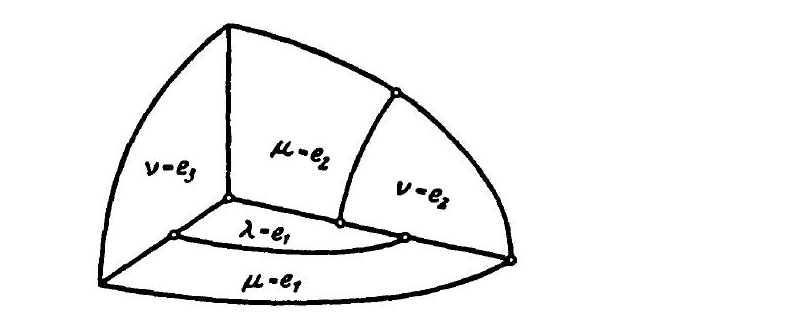
\includegraphics[width=.52\textwidth]{figures/ch04_fig1.png}\\[-0.3em]
{\small Figure 1. Confocal surfaces of the second order.}
\end{center}
Now if $\omega$ and $\omega'$ are, respectively, the real and pure imaginary periods of the integrals $t_i$, i.e. if
\[
\omega=2\int_{e_1}^{\infty}\frac{d\lambda}{\sqrt{f(\lambda)}},\qquad
\omega'=2\int_{-\infty}^{e_3}\frac{d\lambda}{\sqrt{f(\lambda)}},
\]
we may let $t_1$ vary from $0$ to $\omega/2$, $t_2$ from $\omega/2$ to $\tfrac12(\omega+\omega')$, and $t_3$ from $\tfrac12(\omega+\omega')$ to $\tfrac12\omega'$, obtaining all the points of the octant. If the interval for each $t_i$ is doubled the point ranges over the whole space. If a single-valued function of the $t_i$ is to be single-valued in space, it must remain unchanged under all substitutions of the $t_i$ which leave $x,y,$ and $z$ unchanged, for example it is single-valued if $t_1$ and $t_2$ are replaced by $\omega-t_1$ and $\omega-t_2$, respectively.

If we write $t_1=u$, $t_2=\omega/2+iv$, $t_3=\omega'/2+w$, $\wp(t_1)=f(u)$, $\wp(t_2)=g(v)$, $\wp(t_3)=h(w)$, we may take $u,v,$ and $w$ to be real. Then
\begin{align}\tag{71}
ds^2={}&[f(u)-g(v)][f(u)-h(w)]\,du^2\notag\\
&+[f(u)-g(v)][g(v)-h(w)]\,dv^2\notag\\
&+[f(u)-h(w)][g(v)-h(w)]\,dw^2
\end{align}
and for real $u,v,w$ all the coefficients are non-negative, since $f(u)\ge e_1\ge g(v)\ge e_2\ge h(w)\ge e_3$. The fact that $dt_2$ is pure imaginary in the symmetric form in $t_1,t_2,t_3$ is important; for, the positive definite character of $ds^2$ is assured by the negative value of the coefficient of $dt_2^2$.

Among the \emph{degenerate forms of ellipsoidal coordinates} we may mention (aside from spherical coordinates, which may also be regarded as a degenerate case) the \emph{spheroidal and paraboloidal coordinates}. If two of the $e_i$, say $e_1$ and $e_2$, coincide we obtain
\begin{equation}\tag{72}
\frac{x^2+y^2}{s-e_1}+\frac{z^2}{s-e_3}=1.
\end{equation}
The two roots $s=\lambda_1$, $s=\lambda_2$ of this equation, together with the angle $\varphi$ defined by
\[
x=r\cos\varphi,\qquad y=r\sin\varphi,\qquad r^2=x^2+y^2,
\]
form the new coordinates. We have here
\begin{equation}\tag{73}
r^2=\frac{(\lambda_1-e_1)(\lambda_2-e_1)}{e_3-e_1},\qquad
z^2=\frac{(\lambda_1-e_3)(\lambda_2-e_3)}{e_1-e_3},
\end{equation}
\begin{align}\tag{74}
ds^2={}&r^2d\varphi^2+\frac{\lambda_1-\lambda_2}{4(\lambda_1-e_1)(\lambda_1-e_3)}\,d\lambda_1^2
+\frac{\lambda_2-\lambda_1}{4(\lambda_2-e_1)(\lambda_2-e_3)}\,d\lambda_2^2\notag\\
={}&r^2d\varphi^2+(\lambda_1-\lambda_2)(dt_1^2-dt_2^2)
\end{align}
with
\begin{equation}\tag{75}
t_i=\int^{\lambda_i}\frac{d\lambda}{\sqrt{4(\lambda-e_1)(\lambda-e_3)}}.
\end{equation}
Hence
\begin{equation}\tag{76}
\Delta T=\frac1{r^2}\frac{\partial^2T}{\partial\varphi^2}
+\frac1{r(\lambda_1-\lambda_2)}\left[\frac{\partial}{\partial t_1}\left(r\frac{\partial T}{\partial t_1}\right)-\frac{\partial}{\partial t_2}\left(r\frac{\partial T}{\partial t_2}\right)\right].
\end{equation}
If we now let one end of the ellipsoids tend to infinity we obtain, after passage to the limit,\footnote{These coordinates may, of course, also be defined without reference to the foregoing treatment by starting out from the system (77) of confocal paraboloids of revolution.} the \emph{paraboloidal coordinates} as the roots $\lambda_1,\lambda_2$ of equation
\begin{equation}\tag{77}
\frac{x^2+y^2}{s-e_1}-2z+s-e_1=0,
\end{equation}
where $r$ and $z$ are given by the following expressions:
\begin{equation}\tag{78}
r^2=-(\lambda_1-e_1)(\lambda_2-e_1),\qquad 2z=2e_1-\lambda_1-\lambda_2.
\end{equation}
Here the coordinates of a point in space are $\lambda_1,\lambda_2,$ and $\varphi$. The line element is (74)
\[
ds^2=r^2d\varphi^2+\frac{\lambda_1-\lambda_2}{4(\lambda_1-e_1)}\,d\lambda_1^2
+\frac{\lambda_2-\lambda_1}{4(\lambda_2-e_1)}\,d\lambda_2^2
=r^2d\varphi^2+(\lambda_1-\lambda_2)(dt_1^2-dt_2^2)
\]
with
\begin{equation}\tag{79}
t_i=\int^{\lambda_i}\frac{d\lambda}{\sqrt{4(\lambda-e_1)}}=\sqrt{\lambda_i-e_1},
\end{equation}
and the differential expression $\Delta T$ takes the form (76)
\[
\Delta T=\frac1{r^2}\frac{\partial^2T}{\partial\varphi^2}
+\frac1{r(\lambda_1-\lambda_2)}\left[\frac{\partial}{\partial t_1}\left(r\frac{\partial T}{\partial t_1}\right)-\frac{\partial}{\partial t_2}\left(r\frac{\partial T}{\partial t_2}\right)\right].
\]
If in the above expressions the terms containing $\varphi$ are omitted, one is immediately led to the formulas for elliptic and parabolic coordinates in the $r,z$-plane. In both cases we obtain, from formula (64),
\[
\Delta T=\frac1{\lambda_1-\lambda_2}\left(\frac{\partial^2T}{\partial t_1^2}-\frac{\partial^2T}{\partial t_2^2}\right),
\]
in which $\lambda_i$ and $t_i$ are connected by
\[
t_i=\int^{\lambda_i}\frac{d\lambda}{\sqrt{4(\lambda-e_1)(\lambda-e_3)}}
\]
and
\[
t_i=\sqrt{\lambda_i-e_1},
\]
respectively.

\section{Transformation of Variational Problems to Canonical and Involutory Form}
The Lagrange multiplier method leads to several transformations which are important both theoretically and practically.\footnote{See E. Trefftz, Ein Gegenst\"uck zum Ritzschen Verfahren, \emph{Verh. d. 2. Int. Kongr. f\"ur Technische Mechanik}, Z\"urich, 1927, p. 131, where such an approximation procedure was first given. See also Trefftz, Konvergenz und Fehlersch\"atzung beim Ritzschen Verfahren, \emph{Math. Ann.}, Vol. 100, 1928, pp. 503--521.}

By means of these transformations new problems equivalent to a given problem can be so formulated that stationary conditions occur simultaneously in equivalent problems. In this way we are led to transformations of the variational problems which are important because of their symmetric character. Moreover, for a given minimum problem with minimum $d$, we shall often be able to find an equivalent maximum problem with the same value $d$ as maximum; this is a useful tool for the practical problem of bounding $d$ from above and below.

\subsection{Transformation of an Ordinary Minimum Problem with Subsidiary Conditions}
Before discussing these transformations, we briefly consider ordinary minimum problems with a finite number of variables. Our discussion is based on the following self-evident principle: \emph{If a function $f(x_1,x_2,\ldots,x_n)$, subject to certain subsidiary conditions, has a stationary value at the point $x_i=\xi_i$ $(i=1,2,\ldots,n)$ and if the quantities $\xi_i$ satisfy any relation $r(\xi_1,\xi_2,\ldots,\xi_n)=0$, then $f$ remains stationary at $x_i=\xi_i$ provided the additional condition $r(x_1,x_2,\ldots,x_n)=0$ is appended to the subsidiary conditions.}

We begin by considering the problem

I: \emph{$f(x,y)$ is to be made stationary under the subsidiary condition $g(x,y)=0$; the ordinary continuity and differentiability requirements are to be satisfied, and we suppose that $g_x^2+g_y^2\ne0$ at the stationary point.}

By the multiplier rule, problem I may be replaced by the equivalent problem

II: \emph{$F(x,y;\lambda)=f(x,y)+\lambda g(x,y)$ is to be made stationary as a function of the three arguments $x,y,\lambda$.}

The condition $dF=0$ is then equivalent to the three equations $f_x+\lambda g_x=0$, $f_y+\lambda g_y=0$, $g=0$. Had we started with problem II, then by adding explicitly the condition $g=0$, which is automatically fulfilled by the solution of problem II, we would immediately have arrived at problem I by our general principle.

But we may also obtain another problem equivalent to problem II (by equivalence we mean that stationary behavior occurs at the same point) by appending as subsidiary conditions, not $g=0$, but the other two equations which the solution of II satisfies. We thus arrive at problem

III: \emph{$F(x,y;\lambda)=f+\lambda g$ is to be made stationary under the subsidiary conditions $f_x+\lambda g_x=0$, $f_y+\lambda g_y=0$.}

If we assume that the latter two equations can be solved, in the vicinity of the stationary point, for $x$ and $y$ as functions of $\lambda$, then $F(x,y;\lambda)$ goes over into a function $\psi(\lambda)$ of $\lambda$ and we obtain problem IV, which once again is equivalent to the other three problems:

IV: \emph{$\psi(\lambda)$ is to be made stationary.}

We shall now investigate the stationary points; are they or are they not maxima or minima? Let us suppose in problem I, henceforth denoted by I$'$, that $f$ possesses an actual minimum $f(\bar x,\bar y)=d$ at the point $\bar x,\bar y$. We then consider problem

II$'$: \emph{$F(x,y;\lambda)=f+\lambda g=\min.$ with fixed $\lambda$.} Let us assume that, if $\lambda$ is chosen arbitrarily in a certain neighborhood of the value $\bar\lambda$ defined by the Lagrange multiplier rule, there exists an actual minimum, which we denote by $d_\lambda=\psi(\lambda)$, and which is characterized by the equations $f_x+\lambda g_x=0$, $f_y+\lambda g_y=0$. Then we certainly have
\[
d_\lambda\le d.
\]
Indeed, problem I$'$ with the minimum $d$ is obtained from problem II$'$ with minimum $d_\lambda$ by appending the condition $g=0$, which restricts the domain of comparison values. If we further assume that for every $\lambda$ in the neighborhood of $\bar\lambda$ the equations $f_x+\lambda g_x=0$, $f_y+\lambda g_y=0$ uniquely determine $x$ and $y$ as functions of $\lambda$, then $d_{\bar\lambda}=d$, and
\[
d=\max(d_\lambda).
\]
Thus $d$ is the maximum of the minimum $\psi(\lambda)$ of $F^*=f+\lambda g$ where the minimum is to be taken for fixed $\lambda$ and then the maximum taken with respect to $\lambda$. Under these conditions we may also characterize $d$ by the problem

III$'$: \emph{$F(x,y;\lambda)=f+\lambda g=\max.=d$ subject to the subsidiary conditions $f_x+\lambda g_x=0$, $f_y+\lambda g_y=0$.}

The problem $f=(x+1)^2+y^2=\min.$ subject to the condition $g=2x=0$ may serve as an illustration of our maximum-minimum considerations. Geometrically the problem is to find the lowest point or vertex of the vertical parabola which is formed by the intersection of the paraboloid $z=(x+1)^2+y^2$ with the plane $x=0$. We obtain immediately the value $d=1$ of the desired least value of $z=(x+1)^2+y^2$. We now note that for fixed $\lambda$ the paraboloid
\[
z=f+\lambda g=(x+\lambda+1)^2+y^2-2\lambda-\lambda^2
\]
always contains the above parabola and that the vertex of the paraboloid lies lower than that of the parabola. By varying $\lambda$ we vary the vertex of the paraboloid which will at most move up to the vertex of the parabola but never any higher. Thus the vertex of the parabola is the highest point of the set of lowest points of our paraboloids.

\subsection{Involutory Transformation of the Simplest Variational Problems}
Analogous transformations of variational problems are based upon the following general principle: \emph{If a functional $J[u,v,\ldots]$ is stationary for a certain admissible system of functions $u,v,\ldots$, which may be required to fulfill certain subsidiary conditions, then $J$ remains stationary for this system of functions when the set of subsidiary conditions is enlarged to include any further relations already satisfied by the functions $u,v,\ldots$.}

We shall call conditions that are necessary for the vanishing of the variation (such as the Euler equations and the natural boundary conditions) \emph{natural conditions}; subsidiary and boundary conditions imposed a priori will be known as \emph{constraints}. Then, from our principle: \emph{If a variational problem for a given functional is changed by the explicit addition of one or more natural conditions to the set of constraints, the stationary character of the functional is not affected.}

We shall now turn to some problems of the simplest type:

I: $J=\int_{x_0}^{x_1}F(x,u,u')\,dx$ \emph{is to have a stationary value subject to the usual continuity conditions, the boundary conditions}
\begin{equation}\tag{80}
u(x_0)-u_0=0,\qquad u(x_1)-u_1=0,
\end{equation}
\emph{and the subsidiary condition}
\begin{equation}\tag{81}
\frac{du}{dx}-u'=0.
\end{equation}
That is, we regard the variational problem as one involving two unknown functions $u$ and $u'$ subject to the differential equation of constraint (81). In accordance with the multiplier rule the solutions of I are simultaneously solutions of the following problem
\[
\text{II:}\quad H[u,u',\lambda;\mu_0,\mu_1]
=\int_{x_0}^{x_1}\left[F+\lambda\left(\frac{du}{dx}-u'\right)\right]dx
-\mu_0[u(x_0)-u_0]+\mu_1[u(x_1)-u_1]
\]
\emph{is to be made stationary, where $u(x)$, $u'(x)$, $\lambda(x)$ and the parameters $\mu_0$ and $\mu_1$ are to be determined, and there are no subsidiary or boundary conditions; i.e. the problem is free.} The variational equations, i.e. the Euler equations and the natural boundary conditions of the problem, are
\begin{equation}\tag{82}
F_{u'}-\lambda=0,
\end{equation}
\begin{equation}\tag{83}
F_u-\frac{d\lambda}{dx}=0,
\end{equation}
\begin{equation}\tag{84}
\frac{du}{dx}-u'=0
\end{equation}
in the interior of the interval, and
\begin{equation}\tag{85}
\lambda(x_0)+\mu_0=0,\qquad \lambda(x_1)+\mu_1=0,
\end{equation}
\begin{equation}\tag{86}
u(x_0)-u_0=0,\qquad u(x_1)-u_1=0
\end{equation}
at the end points, as is found immediately when the first variation is set equal to zero. If we eliminate $\lambda,\mu_0,\mu_1$, we obtain the Euler equation.

If we apply our general principle to problem II by appending to the set of constraints the conditions $du/dx-u'=0$, $u(x_0)-u_0=0$, $u(x_1)-u_1=0$, we are led back to problem I. If, on the other hand, we adjoin equations (82), (83), (85), which correspond to the natural conditions of problem I, we obtain a transformation which is of importance in applications; we shall call it the \emph{transformation into the reciprocal form of the variational problem}.\footnote{The significance of this transformation was first discovered by K. O. Friedrichs, Ein Verfahren der Variationsrechnung, \emph{Nachr. der Ges. d. Wiss.}, G\"ottingen, 1929, pp. 13--20.} In this way we obtain problem III, which may be expressed as a problem of type I if we remove the derivative $du/dx$ from the integral $H$ by partial integration and then introduce new argument functions $p,p'$ and a new integrand $\Psi(x,p,p')$ by means of equations
\begin{equation}\tag{87}
F_{u'}=p,\qquad F_u=p',\qquad pu'+p'u-F=\Psi.
\end{equation}

In order that this ``Legendre transformation'' be meaningful we must require that $u$ and $u'$ can be obtained from the first two equations as functions of $p,p',$ and $x$; these functions are then to be substituted in the left side of the third equation. This procedure certainly can be carried out, if the requirement
\begin{equation}\tag{88}
F_{u'u'}F_{uu}-(F_{uu'})^2\ne0
\end{equation}
is fulfilled for all sets of values $x,u,u'$ of the fundamental domain. We thus obtain the following ``reciprocal'' problem,\footnote{This may be regarded as the analogue of problem IV of subsection 1.} equivalent to I,
\[
\text{IV:}\quad -\int_{x_0}^{x_1}\Psi(x,p,p')\,dx+p(x_1)u_1-p(x_0)u_0
\]
\emph{is to be made stationary under the subsidiary condition}
\[
\frac{dp}{dx}-p'=0;
\]
\emph{no boundary conditions are imposed.}

The natural conditions for problem IV are
\[
\frac{d}{dx}\Psi_{p'}-\Psi_p=0
\]
in the interior and
\[
\Psi_{p'}\big|_{x_0}-u_0=0,\qquad \Psi_{p'}\big|_{x_1}-u_1=0
\]
on the boundary. It is apparent from their derivation that these constraints are identical with those of problem I; this may be independently verified with the help of the inversion
\[
\Psi_{p'}=u,\qquad \Psi_p=u',\qquad up'+u'p-\Psi=F
\]
of the Legendre transformation (87).

By use of the same formulas we see that the reciprocal transformation applied to the free problem IV leads back to the original problem I. \emph{Thus this transformation is of involutory character, and the natural conditions of the one problem go over into the constraints of the other.}

The degenerate case in which the integrand $F$ of the variational problem does not depend on $u$ explicitly or contains $u$ only linearly requires special treatment. We have here
\[
F(x,u,u')=g(x,u')+u f(x).
\]

In this case the Legendre transformation considered previously is not reversible for arbitrary $p$ and $p'$. But by applying our transformation principle directly we find that the following variational problem is equivalent to the original problem I:
\[
-\int_{x_0}^{x_1}\Phi(p)\,dx+p(x_1)u_1-p(x_0)u_0=\text{stationary},
\]
with the subsidiary condition $dp/dx=f(x)$. Here $p$ and $\Phi(p)$ are related to the expressions in the original problem by the transformation
\[
p=g_{u'},\qquad -\Phi(p)=g(x,u')-u'p,
\]
and it is assumed that the equation $g_{u'}=p$ can be solved for $u'$ in terms of $p$. The new problem is essentially simpler than the original one in the following respect: the required function $p(x)$ can be obtained, aside from an additive parameter, by quadrature from the subsidiary condition. Thus in this degenerate case the variational problem goes over into an ordinary extremum problem of determining a parameter.

As in subsection 1 we now examine the effect of these transformations upon the maximum or minimum character of our expressions.

By repeating the arguments of subsection 1, we shall arrive at the following result: \emph{If the original problem I (henceforth to be denoted by I$'$) pertains to a minimum $d$, then the same value $d$ will occur as a maximum in the corresponding reciprocal problem IV (to be denoted by IV$'$).}

Again, this statement is true only if certain restrictions are imposed. We require, specifically, that for any arbitrary $\lambda(x)$ with a piecewise continuous derivative, for which $\lambda(x_1)+\mu_1=0$, $\lambda(x_0)+\mu_0=0$,\footnote{Without this condition, which is automatically satisfied by the solution, it would certainly be impossible to obtain a minimum with arbitrary $\lambda,\mu$.} the expression $H$ of problem II, page 234, possesses a minimum $d_\lambda$ depending on $\lambda$. Then, removing the derivative of $u$ by partial integration, we obtain problem
\[
\begin{aligned}
H&=\int_{x_0}^{x_1}\left[F+\lambda\left(\frac{du}{dx}-u'\right)\right]dx\\
&\qquad-\mu_0\bigl(u(x_0)-u_0\bigr)+\mu_1\bigl(u(x_1)-u_1\bigr)
\end{aligned}
\]
\[
\text{II$'$:}\qquad
=\int_{x_0}^{x_1}\left[F-\frac{d\lambda}{dx}u-\lambda u'\right]dx-\lambda(x_0)u_0+\lambda(x_1)u_1
\]
is to be made a minimum, $\lambda(x)$ being a fixed function. The functions $u(x),u'(x)$ that solve this problem then satisfy equations
\begin{equation}\tag{89}
F_{u'}-\lambda=0,\qquad F_u-\frac{d\lambda}{dx}=0.
\end{equation}

We now assume, in analogy with the procedure of subsection 1, that these equations determine the functions $u$ and $u'$ uniquely for arbitrary values of $\lambda$ and $d\lambda/dx$.

Since problem I$'$ arises from problem II$'$ when we impose the additional subsidiary conditions $du/dx-u'=0$, $u(x_0)-u_0=0$, $u(x_1)-u_1=0$, we certainly have $d\ge d_\lambda$.

On the other hand equations (89) are satisfied by the solution of problem I$'$ with $\lambda=\bar\lambda=F_{u'}$ and, because of the assumption of uniqueness, we have $d_{\bar\lambda}=d$.

It follows that
\[
d=\max d_\lambda.
\]
But the problem of maximizing $d_\lambda$ is just the problem IV$'$, and thus our assertion is proved.

A sufficient criterion for the validity of our assumptions is that the inequalities
\begin{equation}\tag{90}
F_{u'u'}F_{uu}-(F_{uu'})^2>0,\qquad F_{u'u'}>0
\end{equation}
hold for all $u$ and $x$ in the domain under discussion and for arbitrary $u'$. As we have already seen (page 216), if these inequalities hold a solution of the Euler equations furnishes a minimum for problem I$'$. The existence of a minimum $d_\lambda$ in problem II$'$ follows from these inequalities similarly; for, equations (89) and inequalities (90) together express the fact that at each value of $x$ the integrand of $H$ possesses a minimum for the appropriate values of $u$ and $u'$. Certainly, then, $H$ itself is a minimum.

In conclusion we may point out that the transition from a minimum problem to a maximum problem, as accomplished by the reciprocal transformation, may be exhibited directly under assumption (90). In the following reasoning, the reciprocal transformation will be obtained once more. From Taylor's expansion, in view of the inequalities (90), we obtain at once the inequality
\[
F(u,u')-F(v,v')-(u-v)F_v-(u'-v')F_{v'}\ge0,
\]
in which the equality holds if and only if $u=v$, $u'=v'$. If we write the above expression in the form
\[
F(u,u')-[F(v,v')-vF_v-v'F_{v'}]-uF_v-u'F_{v'}
\]
and replace $v$ and $v'$ by the quantities $p$ and $p'$ by means of the Legendre transformation
\[
p=F_{v'},\qquad p'=F_v,\qquad \Psi(x,p,p')=vp'+v'p-F,
\]
the inequality becomes
\[
F(x,u,u')+\Psi(x,p,p')-up'-u'p\ge0
\]
for arbitrary $u,u',p,p'$; equality occurs if and only if $p$ and $p'$ correspond to the functions $v=u$, $v'=u'$. We now integrate this inequality between the limits $x_0$ and $x_1$, regarding $u,u',p,p'$ as functions of $x$ subject to the constraints
\[
\frac{du}{dx}-u'=0,\qquad \frac{dp}{dx}-p'=0,\qquad
u(x_0)-u_0=0,\qquad u(x_1)-u_1=0.
\]
The left side can certainly not be negative; it vanishes if and only if $u$ is the solution of problem I$'$ and $p$ the solution of problem IV$'$. Thus the problem
\[
\int_{x_0}^{x_1}[F+\Psi-up'-u'p]dx
\]
\[
=\int_{x_0}^{x_1}F\,dx+\int_{x_0}^{x_1}\Psi\,dx+u_0p(x_0)-u_1p(x_1)=\min.
\]
with the given constraints possesses this solution, and the minimum value in this problem is zero. This statement is equivalent to the above assertion concerning the relation of the two problems I$'$ and IV$'$.

\subsection{Transformation of Variational Problems to Canonical Form}
The general principle formulated in subsection 2 leads to another well-known transformation, the \emph{transformation into canonical form}. Here the Euler second order differential equation is replaced by a system of differential equations of first order. This transformation, which has no exact counterpart in subsection 1, is obtained by imposing equations (82) and (86) as constraints in problem II. Thus one first obtains the problem
\[
\text{IIa:}\qquad \int_{x_0}^{x_1}\left[F(x,u,u')+F_{u'}\left(\frac{du}{dx}-u'\right)\right]dx
\]
is to be made stationary with the boundary conditions $u(x_0)=u_0$, $u(x_1)=u_1$, where $u$ and $u'$ are to be regarded as two independent argument functions.

If we introduce a new argument function\footnote{Thus $p$ is equal to the multiplier occurring in II.}
\[
p=F_{u'}
\]
in place of $u'$ and a new integrand
\[
\Phi(x,u,p)=pu'-F(x,u,u')
\]
in place of $F(x,u,u')$---we expressly assume
\[
F_{u'u'}\ne0,
\]
so that $u'$ can be determined as a function of $p,u,$ and $x$ from the relation $p=F_{u'}$---we obtain the equivalent problem
\[
\text{IIb:}\qquad \int_{x_0}^{x_1}\left[p\frac{du}{dx}-\Phi(x,u,p)\right]dx=\text{stationary}
\]
with the boundary conditions $u(x_0)=u_0$, $u(x_1)=u_1$. It is easily seen that the quantities occurring in the equivalent problems I and IIb are connected by the Legendre transformation
\[
F_{u'}=p,\qquad pu'-F=\Phi,
\]
whose inverse is expressed by the equations
\[
\Phi_p=u',\qquad pu'-\Phi=F.
\]
This form of the variational problem is known as the \emph{canonical form}. The formulation of the variational equations for $p$ and $u$ yields the \emph{canonical differential equations} of the variational problem:
\[
\frac{dp}{dx}+\Phi_u=0,\qquad \frac{du}{dx}-\Phi_p=0.
\]

In an analogous manner we may transform a variational problem for $n$ unknown functions $u_1(x),u_2(x),\ldots,u_n(x)$ of the independent variable $x$ into canonical form.

Summarizing the above discussion, we state without explicitly repeating qualifying sufficient conditions: Suppose, in problem I, $d$ is a minimum; then, in the canonical problem, $d$ becomes a maximum-minimum if for fixed $p$ we find a minimum by varying $u$ and then determine the maximum of this minimum (a function of $p$) by varying $p$.

\subsection{Generalizations}
Our transformation theory is easily extended to problems involving several unknown functions, higher derivatives, or several independent variables. We confine ourselves here to the treatment of a particularly simple example which corresponds to the degenerate case of subsection 2, namely the transformation of Dirichlet's classical variational problem
\[
\text{I:}\qquad \frac12\iint_G\left[\left(\frac{\partial u}{\partial x}\right)^2+\left(\frac{\partial u}{\partial y}\right)^2\right]dx\,dy=\min.
\]
in which $u$ is a function of $x,y$ with piecewise continuous derivatives in the region $G$ and prescribed boundary values $\bar u=f(s)$. The boundary $\Gamma$ of $G$ is assumed to be a curve with continuously turning tangent (except possibly at a finite number of points) and with arc length $s$.

If in problem I we replace the two partial derivatives by the functions $p$ and $q$ and append the subsidiary conditions $\partial u/\partial x=p$, $\partial u/\partial y=q$, the multiplier rule immediately leads to the equivalent problem
\[
\text{II:}\quad \iint_G\left[\frac12(p^2+q^2)+\lambda\left(\frac{\partial u}{\partial x}-p\right)+\mu\left(\frac{\partial u}{\partial y}-q\right)\right]dx\,dy
-\int_\Gamma \rho(s)[\bar u-f(s)]ds=\text{stat.}
\]
Here $\lambda(x,y),\mu(x,y),\rho(s)$ are multipliers. Transforming the double integral by partial integration we obtain II in the form
\[
\iint_G\left[\frac12(p^2+q^2)-u\left(\frac{\partial\lambda}{\partial x}+\frac{\partial\mu}{\partial y}\right)-\lambda p-\mu q\right]dx\,dy
\]
\[
+\int_\Gamma\left[\bar u\left(\bar\lambda\frac{\partial x}{\partial n}+\bar\mu\frac{\partial y}{\partial n}-\rho(s)\right)+\rho(s)f(s)\right]ds=\text{stat.}
\]
Here $\partial/\partial n$ denotes differentiation with respect to the outer normal, and boundary values are indicated by a bar $(\bar u,\bar\lambda,\bar\mu)$. We now impose as explicit subsidiary conditions the Euler differential equations and certain natural boundary conditions:
\[
p-\lambda=0,\qquad q-\mu=0,
\]
\[
\frac{\partial\lambda}{\partial x}+\frac{\partial\mu}{\partial y}=0,\qquad
\bar\lambda\frac{\partial x}{\partial n}+\bar\mu\frac{\partial y}{\partial n}-\rho=0,
\]
thus obtaining the equivalent problem
\[
\text{III:}\qquad -\frac12\iint_G(p^2+q^2)dx\,dy+\int_\Gamma\rho(s)f(s)ds=\text{stat.}
\]
with the subsidiary conditions
\[
\rho(s)-\bar p\frac{\partial x}{\partial n}-\bar q\frac{\partial y}{\partial n}=0
\]
on the boundary and
\[
\frac{\partial p}{\partial x}+\frac{\partial q}{\partial y}=0
\]
in the interior. The reciprocal transformation is completed.

We can simplify the result if we satisfy the latter subsidiary conditions by introducing a function $v(x,y)$ such that
\[
p=\frac{\partial v}{\partial y},\qquad q=-\frac{\partial v}{\partial x}.
\]
Then
\[
\bar p\frac{\partial x}{\partial n}+\bar q\frac{\partial y}{\partial n}=\frac{\partial v}{\partial s},
\]
where the differentiation on the right is to be performed in the direction of the positive tangent of $\Gamma$; the problem goes over into problem
\[
\text{IV:}\qquad -\frac12\iint_G\left[\left(\frac{\partial v}{\partial x}\right)^2+\left(\frac{\partial v}{\partial y}\right)^2\right]dx\,dy
+\int_\Gamma\frac{\partial v}{\partial s}f(s)ds=\text{stat.}
\]
The boundary integral on the right, incidentally, may be transformed by partial integration into the form
\[
-\int_\Gamma v f'(s)\,ds.
\]
In this new problem, the integrand is of the same form as in problem I. The solution of problem I defines a function satisfying the potential equation $\Delta u=\partial^2u/\partial x^2+\partial^2u/\partial y^2=0$ with the boundary values $f(s)$; problem IV also defines a potential function $v$ which, in virtue of the natural boundary conditions, turns out to be the potential function conjugate to $u$.

A minimum in problem I corresponds to a maximum having the same value in problem IV. This becomes clear if we subtract the expression IV from I; a simple transformation leads to the expression
\[
\iint_G\left[\left(\frac{\partial u}{\partial x}-\frac{\partial v}{\partial y}\right)^2+\left(\frac{\partial u}{\partial y}+\frac{\partial v}{\partial x}\right)^2\right]dx\,dy.
\]
Problems I and IV together are equivalent to the problem of minimizing this last integral subject to the single boundary condition $\bar u=f(s)$. The minimum has the value zero and is attained when $u$ is the solution of the appropriate boundary value problem of potential theory and $v$ is its conjugate function satisfying the differential equations
\[
\frac{\partial u}{\partial x}=\frac{\partial v}{\partial y},\qquad
\frac{\partial u}{\partial y}=-\frac{\partial v}{\partial x}.
\]
For a more direct and general treatment of reciprocal quadratic variational problems see \S11.

\section{Variational Calculus and the Differential Equations of Mathematical Physics}
\subsection{General Remarks}
The calculus of variations is a reliable guide both in formulating and in treating differential equations of mathematical physics. Problems of (stable) equilibrium are governed by the variational principle of the \emph{minimum potential energy}; the laws of motion are most simply formulated in terms of \emph{Hamilton's variational principle}. By these two principles we shall derive some of the fundamental differential equations of mathematical physics.

Let us first consider a system with a finite number, say $n$, of degrees of freedom. Let the position of the system be characterized by the values of $n$ parameters $q_1,q_2,\ldots,q_n$; the object is to determine these as functions of the time $t$. We suppose that the mechanical properties of the system are determined by two quantities, the kinetic and potential energy. We assume that the kinetic energy $T(\dot q_1,\dot q_2,\ldots,\dot q_n,q_1,q_2,\ldots,q_n,t)$ is a known function of the $n$ velocities $\dot q_i$, the $n$ coordinates $q_i$, and the time $t$, specifically that it is a quadratic form in the velocities:
\[
T=\sum_{i,k=1}^n P_{ik}(q_1,q_2,\ldots,q_n,t)\dot q_i\dot q_k.
\]
The potential energy $U(q_1,q_2,\ldots,q_n,t)$ is assumed to be a known function of $t$ and the coordinates $q_i$. Then Hamilton's principle states: \emph{Between two instants of time $t_0$ and $t_1$ the motion proceeds in such a way that for the functions $q_i(t)$ the integral}
\[
J=\int_{t_0}^{t_1}(T-U)\,dt
\]
\emph{is stationary in comparison with the neighboring functions $\bar q_i(t)$ for which $\bar q_i(t_0)=q_i(t_0)$ and $\bar q_i(t_1)=q_i(t_1)$. In other words: The actual motion makes the value of the integral $J$ stationary with respect to all neighboring virtual motions which lead from the initial to the final position of the system in the same interval of time.}

In accordance with \S3 Hamilton's principle leads at once to Lagrange's general equations of motion
\begin{equation}\tag{91}
\frac{d}{dt}\frac{\partial T}{\partial\dot q_i}-\frac{\partial}{\partial q_i}(T-U)=0\qquad(i=1,2,\ldots,n).
\end{equation}
The equilibrium conditions can be obtained from the equations of motion, under the assumption that $T$ and $U$ do not depend explicitly on $t$, by setting the derivatives with respect to time equal to zero in (91). The resulting conditions are
\begin{equation}\tag{92}
\frac{\partial U}{\partial q_i}=0.
\end{equation}
Thus: A mechanical system with the potential energy $U(q_1,q_2,\ldots,q_n)$ is in equilibrium at a particular set of values of the coordinates $q_1,q_2,\ldots,q_n$ if and only if the potential energy is stationary for this set of values.

In order that the equilibrium be stable, it is, moreover, necessary and sufficient that the stationary value of $U$ in the equilibrium position be a minimum.

This fact follows easily from the principle of conservation of energy, $T+U=\text{const.}$, an immediate consequence of equations (91). We shall henceforth accept the principle of minimum potential energy as the condition of stable equilibrium.

A motion takes on a particularly simple character if confined to the vicinity of a stable equilibrium position of a system. We may assume without loss of generality that at the equilibrium in question all the coordinates $q_i$ vanish. If we now consider those motions close to the equilibrium position for which higher powers of the coordinates and of their time derivatives are negligible compared with lower powers, and if we assume that $T$ and $U$ do not contain $t$ explicitly, then we may regard $T$ as a positive definite quadratic form in $\dot q_i$ with constant coefficients $a_{ik}$:
\[
T=\sum_{i,k=1}^n a_{ik}\dot q_i\dot q_k.
\]
Under these hypotheses, $U$ also is a positive definite quadratic form in $q_i$ with the constant coefficients $b_{ik}$:
\[
U=\sum_{i,k=1}^n b_{ik}q_iq_k.
\]
Thus the equations of motion go over into the linear second order differential equations with constant coefficients
\[
\sum_{k=1}^n a_{ik}\ddot q_k+\sum_{k=1}^n b_{ik}q_k=0
\]
which govern ``small vibrations'' about a stable equilibrium position, and which will be discussed in detail in the next chapter.

In the case of problems of continuum mechanics, in which the position of the system no longer can be described by a finite number of variables, we may also proceed from Hamilton's principle or from the principle of least potential energy. Here the kinetic and potential energies are not functions of a finite number of variables, but are functionals represented by integrals over appropriate space regions, surfaces, or lines.

\subsection{The Vibrating String and the Vibrating Rod}
The simplest example of continuum mechanics is given by the homogeneous vibrating string, subjected to a constant tension $\mu$, which executes small transverse vibrations about the position of stable equilibrium, the interval $0\le x\le l$ of the $x$-axis. Our problem is to determine the perpendicular deflection $u(x,t)$ of a point on the string from its equilibrium position. We assume that the motion is ``small'' in the sense, specifically, that higher powers of the function $u$ and of its derivatives may be neglected compared with lower powers. First, let us consider the case in which the string is fixed at its end points, i.e. $u(0,t)=u(l,t)=0$. The kinetic energy of the string is given by the integral
\[
T=\frac12\int_0^l\rho u_t^2\,dx,
\]
where $\rho$ denotes the linear density of the string. The potential energy $U$ is proportional to the increase in length compared with the length at rest, the factor of proportionality being equal to the tension $\mu$. Since, apart from quantities of higher order, the change in length
\[
\int_0^l\sqrt{1+u_x^2}\,dx-l
\]
approximately equals $\frac12\int_0^l u_x^2\,dx$, the potential energy takes the form
\[
U=\frac12\int_0^l\mu u_x^2\,dx.
\]
Hamilton's principle, therefore, leads to the problem of finding an admissible function $u(x,t)$ for which the double integral
\[
\int_{t_0}^{t_1}(T-U)\,dt
=\frac12\int_{t_0}^{t_1}\int_0^l(\rho u_t^2-\mu u_x^2)\,dx\,dt
\]
is stationary compared with all the continuous functions $u(x,t)$ which have piecewise continuous first derivatives, vanish at $x=0$ and at $x=l$, and coincide with the functions $u(x,t_0)$ and $u(x,t_1)$ corresponding to the actual motion at $t=t_0$ and $t=t_1$, respectively. For constant $\rho$ and $\mu$, we then obtain from the general laws of the variational calculus the partial differential equation of the vibrating string
\begin{equation}\tag{93}
\rho u_{tt}-\mu u_{xx}=0.
\end{equation}
If an external force $f(x,t)$ acts on the string the term $\int_0^l f(x,t)u\,dx$ must be added to the potential energy, and we now obtain the differential equation
\begin{equation}\tag{94}
\rho u_{tt}-\mu u_{xx}+f(x,t)=0.
\end{equation}
The stable equilibrium of a string under the influence of an external force is given, in accordance with the minimum principle, by the minimum of the integral $\int_0^l(\frac12\mu u_x^2+fu)\,dx$, where the external force $f(x)$ is, of course, assumed to be time-independent. This leads to the Euler equation
\[
\mu u_{xx}-f(x)=0
\]
as a special case of the equation of motion (94).

We now formulate the corresponding equations for the states of a laterally movable rod. The rod is defined as a one-dimensional continuum, lying in a straight line when at rest, whose potential energy at deformation is proportional to the integral of the square of the curvature, extended over its length. If we again assume that higher powers of the deformation function $u(x,t)$ and of its derivatives are negligible compared with lower powers, we obtain an expression of the form $\frac12\mu\int_0^l u_{xx}^2\,dx$ for the potential energy of deformation. The kinetic energy has the same form as that of the string. With an external force $f(x,t)$ acting, the equation of motion, derived from Hamilton's principle, becomes
\[
\rho u_{tt}+\mu u_{xxxx}+f(x,t)=0,
\]
and the condition for equilibrium under an external force $f(x)$ is
\[
\mu u_{xxxx}+f(x)=0.
\]
The boundary conditions or other constraints to be imposed are of great importance in the solution of our variational problems. We may, for example, fix the boundary by conditions such as $u(0)=u(l)=0$ for the string or $u(0)=u_x(0)=u(l)=u_x(l)=0$ for the rod, or we may instead leave the boundaries free. For free boundaries, the methods of \S5 lead to the natural boundary conditions
\begin{equation}\tag{95}
u_x(0,t)=u_x(l,t)=0
\end{equation}
for the string and
\begin{equation}\tag{96}
u_{xx}(0,t)=u_{xx}(l,t)=0,\qquad u_{xxx}(0,t)=u_{xxx}(l,t)=0
\end{equation}
for the rod.

If the end points of the string are neither fixed nor free but are held by elastic forces, boundary terms $\frac12h_1\mu u^2(0,t)$ and $\frac12h_2\mu u^2(l,t)$ must be added to the potential energy. These terms do not alter the equation of motion (94), but lead to the natural boundary conditions\footnote{For further remarks concerning rods, see \S12, 12--13.}
\[
u_x(0,t)=h_1u(0,t),\qquad u_x(l,t)=-h_2u(l,t).
\]

\subsection{Membrane and Plate}
For the plane membrane and plate the situation is similar to that for the string and rod. A membrane is a portion of a surface, plane at rest, with potential energy proportional to change in area; the proportionality factor is known as the tension. Suppose that the membrane at rest covers a region $G$ of the $x,y$-plane; let the deformation normal to the equilibrium plane be denoted by $u(x,y)$, and suppose this deformation to be small in the sense that higher powers of $u,u_x,u_y$ are negligible compared with lower ones. Then the expression
\[
\iint_G(1+u_x^2+u_y^2)^{1/2}\,dx\,dy
\]
for the area may be replaced by
\[
\iint_G\left[1+\frac12(u_x^2+u_y^2)\right]dx\,dy,
\]
and the required potential energy, apart from a constant factor, is given by the double integral
\begin{equation}\tag{97}
\frac12\iint_G(u_x^2+u_y^2)\,dx\,dy.
\end{equation}

We consider first the equilibrium problem for the membrane. If we suppose that the displacement $u(x,y)$ of the membrane possesses prescribed values $\bar u=\bar u(s)$ on the boundary $\Gamma$ of $G$---where $s$ denotes the arc length of $\Gamma$---and that no external forces act on the membrane, then the equilibrium position is characterized by the following variational problem: The displacement $u(x,y)$ in the equilibrium position is that function for which the integral $\iint_G(u_x^2+u_y^2)dx\,dy$ attains the least possible value if all those functions $u$ are admitted for competition which are continuous in the closed domain $G$, take on the prescribed boundary values $\bar u(s)$, and possess continuous first and piecewise continuous second derivatives\footnote{Later, for the complete treatment of the problem, it will be important that the continuity requirements for the second derivatives may be relaxed without altering the solution.} in the interior. The Euler equation is
\[
\Delta u=u_{xx}+u_{yy}=0.
\]
Thus the problem of finding the equilibrium position is equivalent to the boundary value problem: find in $G$ a solution of the above partial differential equation (the potential equation) which assumes prescribed values on the boundary $\Gamma$ of $G$.

We now make the more general assumptions that the interior of the membrane is subject to an external force of surface density $f(x,y)$, the boundary of the membrane (supposed to be freely movable above $\Gamma$) to an external force of linear density $p(s)$, and, finally, that the boundary is tied to its rest position by elastic forces which are characterized by a modulus of elasticity of linear density $\sigma(s)$. Then the potential energy of a membrane with the displacement $u(x,y)$ is given by the expression
\[
\iint_G\left[\frac12\mu(u_x^2+u_y^2)+fu\right]dx\,dy
+\int_\Gamma\left[p(s)u+\frac12\sigma(s)u^2\right]ds.
\]
Once more we obtain the equilibrium position by finding a function $u(x,y)$, subject to no boundary conditions but only to the above continuity conditions, for which this integral is a minimum. The Euler equation (which expresses the equilibrium condition in the interior) is, if we take $\mu=1$,
\[
\Delta u=f(x,y);
\]
and the natural boundary condition is
\[
\frac{\partial u}{\partial n}+\sigma u+p(s)=0.
\]
These two requirements again represent a boundary value problem for a partial differential equation.

From this general case, we again arrive at the problem of solving the differential equation $\Delta u=f$ with the boundary values $u=0$, if we set $p$ equal to zero and let $\sigma$ increase beyond all bounds.

If $\sigma=0$ our equilibrium problem does not in general possess a solution. Physically, this is plausible; for, a freely movable membrane, subjected to arbitrary external forces, cannot have a stable equilibrium position unless the external forces happen to be balanced. This fact is easily proved from the variational principle: In order that our expression for the energy possess a lower bound in the case $\sigma=0$, equation
\begin{equation}\tag{98}
\iint_G f\,dx\,dy+\int_\Gamma p\,ds=0
\end{equation}
must be satisfied. Indeed, for a constant displacement $u(x,y)=c$, the energy is $c$ times the left side of (98) and can therefore have arbitrarily large negative values, unless the left side vanishes. But if we impose condition (98), the solution of the variational or equilibrium problem is not determined uniquely, since an arbitrary constant can be added to $u$ without altering the value of the energy; its minimum is therefore also unchanged. We must impose a further condition in order to fix the solution uniquely. It is customary to use the condition
\[
\iint_Gu\,dx\,dy=0,
\]
which means that the center of mass of the membrane is fixed in the rest position.

We arrive at the equations of motion of a membrane by Hamilton's principle, noting that the kinetic energy is given by
\begin{equation}\tag{99}
T=\frac12\rho\iint_Gu_t^2\,dx\,dy.
\end{equation}
If external forces act with surface density $f(x,y,t)$ in the interior of the membrane and line density $p(s,t)$ on the boundary, and if the boundary is again subjected to elastic forces with the elastic modulus $\sigma(s)$, Hamilton's principle requires that the expression
\[
\int_{t_0}^{t_1}\iint_G\left[\frac12\rho u_t^2-\frac12\mu(u_x^2+u_y^2)-f(x,y,t)u\right]dx\,dy\,dt
\]
\[
-\int_{t_0}^{t_1}\int_\Gamma\left[\frac12\sigma u^2+pu\right]ds\,dt
\]
be made stationary. The Euler equation for this problem is
\[
\mu\Delta u-\rho u_{tt}-f(x,y,t)=0;
\]
the natural boundary conditions are
\begin{equation}\tag{100}
\sigma u+\mu\frac{\partial u}{\partial n}+p(s,t)=0.
\end{equation}
If the membrane has a fixed boundary, i.e. if the values of $u$ on the boundary are given as a function of the arc length, then the prescription of these boundary values takes the place of condition (100).

In the equilibrium case the minimum principle not only gives the pertinent formulation but also proves a powerful tool for solving and analyzing the problem. However, in dynamic problems the chief use of Hamilton's principle is to derive formally the differential equation; for the further analysis of these equations Hamilton's principle is often not suitable since it requires that the functions admitted for comparison be prescribed at two fixed instants of time $t_0$ and $t_1$, conditions not generally encountered in actual problems. The information usually given in dynamical problems comprises boundary conditions and, in addition, \emph{initial conditions}, i.e. the values of the functions $u(x,y,t)$ and $u_t(x,y,t)$ at one instant $t=0$. Thus dynamic problems lead to mixed boundary and initial value problems.

The situation is analogous in the case of the plate. A plate is an elastic two-dimensional body, plane when in equilibrium, whose potential energy under deformation is given by an integral of a quadratic form in the principal curvatures of the plate. If the principal radii of curvature of the deformed plate are denoted by $\rho_1,\rho_2$ the potential energy density is given by an expression of the form
\[
A\left(\frac1{\rho_1^2}+\frac1{\rho_2^2}\right)+\frac{2B}{\rho_1\rho_2},
\]
where $A$ and $B$ are constants determined by the material of the plate. Assuming $u,u_x,u_y,\ldots$ to be small, we may write
\[
\frac1{\rho_1}+\frac1{\rho_2}=\Delta u=u_{xx}+u_{yy},\qquad
\frac1{\rho_1\rho_2}=u_{xx}u_{yy}-u_{xy}^2.
\]
\ctnote{此处原文将第一式印作 $2/\rho_1+2/\rho_2=\Delta u$。但由紧接着的式 (101) 以及小挠度板的主曲率关系，所需关系应为 $1/\rho_1+1/\rho_2=\Delta u$；原式多出因子 $2$。}
Thus the desired potential energy of deformation is given by an expression of the form
\begin{equation}\tag{101}
U_1=\iint_G\left[(\Delta u)^2-2(1-\mu)(u_{xx}u_{yy}-u_{xy}^2)\right]dx\,dy,
\end{equation}
apart from a constant factor (depending on the material) which we may set equal to unity.

To this must be added the energy due to external surface forces, boundary forces, and bending moments on the boundary if they are prescribed:
\[
U_2=\iint_Gfu\,dx\,dy+\int_\Gamma p(s)u\,ds+\int_\Gamma m(s)\frac{\partial u}{\partial n}\,ds;
\]
here $f(x,y),p(s),m(s)$ represent, respectively, the densities of applied surface forces, boundary forces, and bending moments normal to the boundary curve.

Equilibrium is once more characterized by the requirement that $U_1+U_2$ be a minimum for a suitable admissible function $u(x,y)$. (Here the admissible functions have continuous derivatives up to the fourth order, but these conditions may actually be greatly relaxed without affecting the solution of the problem.) To find the Euler equations and the natural boundary conditions for our minimum problem we must form the variation $\delta U=\delta U_1+\delta U_2$, as outlined in \S5, and equate it to zero. We obtain
\[
\delta U_1=\iint_G(\Delta\Delta u\,\delta u)\,dx\,dy-\int_\Gamma M\,\delta\frac{\partial u}{\partial n}\,ds-\int_\Gamma P\,\delta u\,ds,
\]
with
\[
M(u)=-\Delta u+(1-\mu)(u_{xx}x_s^2+2u_{xy}x_sy_s+u_{yy}y_s^2),
\]
\[
P(u)=\frac{\partial}{\partial n}\Delta u+(1-\mu)\frac{\partial}{\partial s}\left(u_{xx}x_nx_s+u_{xy}(x_ny_s+x_sy_n)+u_{yy}y_ny_s\right).
\]
Here $x_n,y_n$ and $x_s,y_s$ are the direction cosines of the outward normal and the tangent vector, respectively. From the condition $\delta U=0$ we obtain as the equilibrium conditions, the Euler differential equation
\[
\Delta\Delta u+f=0,
\]
and, since no conditions have been imposed a priori on the boundary, the natural boundary conditions\footnote{It is worth noting that in the variational problem for the plate the expression $u_{xx}u_{yy}-u_{xy}^2$, because it is a divergence expression, does not affect the Euler differential equation; yet it is decisive for the form of the natural boundary conditions.}
\[
P(u)-p=0,\qquad M(u)-m=0.
\]
If the plate is clamped at the edge, i.e. if $u$ and $\partial u/\partial n$ have the prescribed value zero at the boundary, these natural boundary conditions are replaced by the conditions $u=0$, $\partial u/\partial n=0$. If the boundary of the plate is supported, i.e. if the boundary is fixed at zero while the tangent plane at the boundary is not constrained, the boundary conditions are
\begin{equation}\tag{102}
u=0,\qquad \Delta u-(1-\mu)(x_s^2u_{xx}+y_s^2u_{yy}+2x_sy_su_{xy})=0.
\end{equation}
To formulate the differential equation for the motion of the plate (the differential equation of the vibrating plate) we again utilize Hamilton's principle, employing the expression (99) for the kinetic energy. We obtain the equations
\[
\mu\Delta\Delta u+\rho u_{tt}=0
\]
or, more generally,
\[
\mu\Delta\Delta u+\rho u_{tt}+f(x,y,t)=0
\]
with appropriate boundary conditions just as above in the equilibrium problems. For the characterization of an actual physical problem these boundary conditions have to be supplemented by initial conditions which describe the initial state, i.e. the functions $u(x,y,0)$ and $u_t(x,y,0)$.

\section{Reciprocal Quadratic Variational Problems}\footnote{This section has been added for the present edition.}
Linear functional equations of mathematical physics result from quadratic variational problems. It is illuminating, especially in regard to the reciprocity phenomenon discussed in \S9, to consider such quadratic problems from a somewhat general and abstract viewpoint (compare Ch. I, \S5, 3) and at the same time to use suggestive geometrical language.\footnote{Recently several authors have rediscovered and advanced the theories indicated in \S9. See J. L. Synge, The method of the hypercircle in function-space for boundary value problems, \emph{Proc. Roy. Soc. London, Ser. A}, Vol. 191, 1941, pp. 447--467; W. Prager and J. L. Synge, Approximations in elasticity based on the concept of function space, \emph{Q. App. Math.}, Vol. 5, 1947, pp. 241--269; J. L. Synge, The method of the hypercircle in elasticity when body forces are present, \emph{Q. App. Math.}, Vol. 6, 1948, pp. 15--19 and the literature quoted there. Synge's papers have called attention to the advantage of a geometrical interpretation from which the distance of the approximations to the exact solutions can be deduced. See also J. B. Diaz and H. J. Greenberg, Upper and lower bounds for the solution of the first boundary value problem of elasticity, \emph{Q. App. Math.}, Vol. 6, 1948, pp. 326--331; H. J. Greenberg, The determination of upper and lower bounds for the solution of the Dirichlet problem, \emph{J. Math. Phys.}, Vol. 27, 1948, pp. 161--182; J. B. Diaz and H. J. Greenberg, Upper and lower bounds for the solution of the first biharmonic boundary value problem, \emph{J. Math. Phys.}, Vol. 27, 1948, pp. 193--201; J. B. Diaz, Upper and lower bounds for quadratic functionals, \emph{Proc. of the Symposium on Spectral Theory and Differential Problems}, Stillwater, 1951.}

We consider, in a linear vector space $\Lambda$ of vectors $p,q,\ldots$, a quadratic form $Q(p,p)$ which we may assume to be positive definite. The vectors may be functions or systems of functions; for example
\[
\text{1)}\qquad Q(p,p)=\iint_G p^2\,dx\,dy
\]
where $p=\operatorname{grad}\varphi(x,y)$ in a region $G$, or
\[
\text{2)}\qquad Q(p,p)=\iint_Gp^2\,dx\,dy
\]
where $p=\Delta\varphi(x,y)$, or a form such as
\[
\text{3)}\qquad Q(p,p)=\int_0^1\int_0^1K(x,y)p(x)p(y)\,dx\,dy.
\]
The definition of the corresponding polar forms $Q(p,q)$ is obvious.

We interpret $Q(p,p)$ as the square of the length of $p$, and call vectors $p,q$ orthogonal if
\[
Q(p,q)=0.
\]
For orthogonal vectors $p,q$ we have
\[
Q(p+q,p+q)=Q(p-q,p-q)=Q(p,p)+Q(q,q)
\]
(``Pythagorean Theorem'').

If $\Omega$ is a linear subspace of the vector space $\Lambda$, we can define another linear subspace $\Sigma$ orthogonal to $\Omega$ as the space of all vectors $\sigma$ orthogonal to all vectors $\omega$ of $\Omega$:
\[
Q(\omega,\sigma)=0.
\]
In all instances considered here the following facts are true: if $\Sigma$ is the linear subspace orthogonal to $\Omega$, then $\Omega$ is the linear subspace orthogonal to $\Sigma$. Every element $p$ in $\Lambda$ can be uniquely decomposed into the sum of ``projections'' $\omega$ and $\sigma$:
\[
p=\omega+\sigma\qquad(\omega\text{ in }\Omega,\ \sigma\text{ in }\Sigma).
\]
If we restrict our vectors by imposing suitable continuity and differentiability conditions, then the theorems which guarantee the existence of a solution for our variational problems also insure the validity of our statements. Accordingly, although we then operate in an incomplete Hilbert space, we assume that the projection theorem holds for the respective incomplete spaces.

We now consider two variational problems.

I: Given two vectors $p_0$ and $q_0$ in $\Lambda$, minimize
\[
Q(p,p)-2Q(p,q_0)
\]
admitting for competition vectors $p$ for which $p-p_0$ is in a prescribed linear subspace $\Omega$. Note that the difference of two admissible vectors belongs to $\Omega$, whereas $p$ itself is restricted to a linear set $\Omega_0$ of vectors ``parallel'' to the linear subspace $\Omega$.

As a first example, let the vector space $\Lambda$ consist of vectors $p$ which are pairs of functions defined in a region $G$; the norm is given by
\[
Q(p,p)=\iint_Gp^2\,dx\,dy.
\]
Take $p_0=\operatorname{grad}\varphi_0$ where $\varphi_0$ is a given function, and take as $\Omega$ the subspace of vectors $\omega=\operatorname{grad}\varphi$ with $\varphi=0$ on the boundary $\Gamma$ of $G$. The subspace $\Sigma$, the orthogonal complement of $\Omega$, consists of those vectors $\sigma$ for which $\operatorname{div}\sigma=0$. If we choose $q_0=0$, then for this example problem I is simply Dirichlet's problem: minimize
\[
\iint_G(\varphi_x^2+\varphi_y^2)\,dx\,dy
\]
subject to the condition $\varphi-\varphi_0=0$ on $\Gamma$.

Next, let the vector space $\Lambda$ consist of functions $p$ defined in a region $G$; the norm is given by
\[
Q(p,p)=\iint_Gp^2\,dx\,dy.
\]
Take $p_0=\Delta\varphi_0$ where $\varphi_0$ is a given function, and take as $\Omega$ the subspace of functions $\omega=\Delta\varphi$ with $\varphi$ and its normal derivative vanishing on $\Gamma$. The subspace $\Sigma$ then consists of those functions $\sigma$ for which $\Delta\sigma=0$. If we choose $q_0=0$, then we have for $\varphi$ the variational problem associated with the clamped plate.

Suppose that $u$ minimizes the functional of problem I. Since $p=u+\varepsilon\omega$ (for any number $\varepsilon$ and any element $\omega$ in $\Omega$) is also admissible, the vanishing of the first variation amounts to the condition
\[
Q(u-q_0,\omega)=0\qquad\text{for all }\omega\text{ in }\Omega.
\]
Hence the equivalent of Euler's equation and the accompanying natural boundary conditions for problem I is that $u-q_0$ is an element of $\Sigma$, the orthogonal complement of $\Omega$.

The uniqueness of the minimizing vector $u$ is now apparent. For, if $u'$ also furnishes a minimum, then, as we have just seen, $u'-q_0$ is in $\Sigma$; consequently $(u-q_0)-(u'-q_0)=u-u'$ is a vector of $\Sigma$. But, in view of the admissibility conditions, $u$ and $u'$ are in $\Omega_0$ so that their difference $u-u'$ lies in $\Omega$. Since the subspaces $\Omega$ and $\Sigma$ contain only the vector zero in their intersection, we see that $u'=u$.

The reciprocal problem to problem I will now be formulated.

II: Minimize the expression
\[
Q(q,q)-2Q(q,p_0)
\]
admitting for competition all vectors $q$ for which $q-q_0$ is in $\Sigma$. If the minimum is attained for $q=v$, then by the same reasoning as above we can conclude that $v-p_0$ is in $\Omega$.

Since $v-q_0$ is in $\Sigma$ and $u-q_0$ is in $\Sigma$, the difference $u-v$ is in $\Sigma$; in the same way, from problem I we see that $v-u$ is in $\Omega$. But since the two orthogonal subspaces have only the vector zero in common, it follows that $u=v$.

Thus problems I and II have the same solutions $u=v$.

By adding to the variational expressions in problems I and II the constant terms $Q(q_0,q_0)$ and $Q(p_0,p_0)$, respectively, we can state the problems in the following form:

I: Find the shortest distance from a fixed vector $q_0$ to the linear set $\Omega_0$, i.e. minimize
\[
d(p)=Q(p-q_0,p-q_0)
\]
over all $p$ in $\Omega_0$.

II: Find the shortest distance from a fixed vector $p_0$ to the linear set $\Sigma_0$, i.e. minimize
\[
d(q)=Q(q-p_0,q-p_0)
\]
over all $q$ in $\Sigma_0$.

Both minima $d_1$ and $d_2$ are attained by the same solution $p=q=u$.

The reciprocal character of the two problems is expressed by the fact that the admissibility conditions of the one are the Euler conditions of the other.

Geometrically, the functions $p$ and $q$ are represented in Figure 2.

A glance at this figure and the theorems of Pythagoras or Thales suggest, moreover, the relations
\[
d_1+d_2=Q(p_0-q_0,p_0-q_0)
\]
and
\[
Q(u-p,u-p)+Q(u-q,u-q)
=4Q\left(u-\frac{p+q}{2},u-\frac{p+q}{2}\right).
\]

where $p,q$ are any two vectors admissible respectively in the two reciprocal problems. These relations follow analytically from the fact that $u-p$ is in $\Omega$, $u-q$ in $\Sigma$; hence $u-p$ and $u-q$ are orthogonal and
\begin{align*}
4Q\left(u-\frac{p+q}{2},u-\frac{p+q}{2}\right)
&=Q(u-p+u-q,u-p+u-q)\\
&=Q(u-p,u-p)+Q(u-q,u-q)\\
&=Q(p-q,p-q).
\end{align*}

\begin{center}
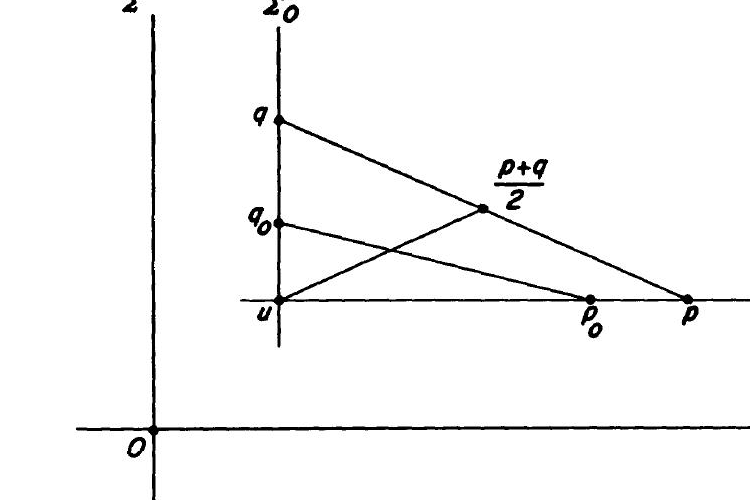
\includegraphics[width=.72\textwidth]{figures/ch04_fig2.png}\\[-0.3em]
{\small Figure 2}
\end{center}

These considerations imply a remarkable fact: an upper bound for one of the two variational problems furnishes at the same time a lower bound for the reciprocal problem, since the sum of the minima is a priori known. This remark will prove relevant in connection with direct methods of the variational calculus.

Furthermore, the second relation,\footnote{In the present connection this relation was pointed out by Synge and Prager.} corresponding to the theorem of Thales, states: The solution $u$ common to both problems deviates from the arithmetical mean of two arbitrary functions $p,q$ admissible, respectively, in the two reciprocal problems by an amount equal to half the distance between the two functions $p$ and $q$. Hence, once $p$ and $q$ are chosen, the sphere of radius $\lvert(p-q)/2\rvert$ about the point $(p+q)/2$ is a geometric locus for $u$.

Special cases (see also \S12, 12) are easily fitted into the general scheme. For example, as we have seen, Dirichlet's problem for the harmonic differential equation in a region $G$ with boundary $\Gamma$ (see \S8) corresponds to
\[
Q(p,p)=\iint_G p^2\,dx\,dy.
\]
The space $\Omega_0$ of $p$ is defined by $p=\operatorname{grad}\varphi(x,y)$, $\varphi-\varphi_0=0$ on $\Gamma$, $p_0=\operatorname{grad}\varphi_0(x,y)$, where $\varphi_0$ is a prescribed function. The space $\Sigma_0=\Sigma$ of $q$ is defined by $\operatorname{div}q=0$, $q_0=0$. Incidentally, it should be noted that in problem II the expression $Q(q,p_0)$ can be transformed into the boundary integral
\[
\int_\Gamma \varphi_0q_n\,ds
\]
where $q_n$ is the normal component of $q$.

Thus the reciprocal problem II can be formulated if we merely know the prescribed boundary values of $\varphi$; no explicit knowledge of a function $\varphi_0(x,y)$ is necessary.

A similar fact is true of other examples, e.g. the problem of the clamped plate, where
\[
Q(p,p)=\iint_Gp^2\,dx\,dy,
\]
\[
p=\Delta\varphi,\qquad p_0=\Delta\varphi_0,\qquad \Delta q=0,\qquad q_0=0,
\]
and where $\varphi-\varphi_0$ and its normal derivative are supposed to vanish on $\Gamma$. Since
\[
Q(q,p_0)=\int_\Gamma\left(\varphi_0\frac{\partial q}{\partial n}-\frac{\partial\varphi_0}{\partial n}q\right)ds,
\]
where $\partial/\partial n$ denotes the normal derivative, problem II actually refers only to the given boundary values of $\varphi$ and $\partial\varphi/\partial n$.

\section{Supplementary Remarks and Exercises}

\subsection{Variational Problem for a Given Differential Equation}
For a given ordinary second order differential equation $y''=f(x,y,y')$ one can always find a function $F(x,y,y')$ such that the equation $[F]_y=0$, when solved for $y''$, is identical with the differential equation.\footnote{Cf. O. Bolza, \emph{Vorlesungen \"uber Variationsrechnung}, Teubner, Leipzig and Berlin, 1909, pp. 37--39.}

\subsection{Reciprocity for Isoperimetric Problems}
The extremals of the problem
\[
J=\int_{x_0}^{x_1}F(x,y,y')\,dx=\text{stationary}
\]
under the condition
\[
K=\int_{x_0}^{x_1}G(x,y,y')\,dx=\text{constant}
\]
are identical with those of the problem $K=\text{stat.}$, $J=\text{const.}$, except for the singular case of \S7, 1.

\subsection{Circular Light Rays}
The following statement is a consequence of this chapter. Suppose light travels in the $x,y$-plane in such a way that its speed is proportional to $y$; then the light rays emitted from any point are circles with their centers on the $x$-axis.

\subsection{The Problem of Dido}
``Dido's problem,'' to enclose the largest possible area of land within a fence of given length, may be generalized by introducing a weight function $\rho(x,y)$ where $\rho(x,y)$ denotes, say, the fertility of the land. The problem is to find a closed curve of given length such that the integral $\iint_G\rho\,dx\,dy$, taken over the enclosed region, assumes its largest possible value. Formulate the differential equation of the extremals.

\subsection{Examples of Problems in Space}
The surface with smallest area which encloses a given volume is the sphere.\footnote{Cf. references to the literature in W. Blaschke, \emph{Kreis und Kugel}, Leipzig, 1916.}

Consider the surface of least area bounded by a given curve which, together with a given surface bounded by the same curve, encloses a prescribed volume; then the extremals are the surfaces of constant mean curvature. If the subsidiary condition concerning the volume is omitted, we arrive at the differential equation of \emph{minimal surfaces} (cf. \S3, 4), which states that the mean curvature is zero.

\subsection{The Indicatrix and Applications}
In finding the extremum of the integral\footnote{Cf. C. Carath\'eodory, \"Uber die starken Maxima und Minima bei einfachen Integralen, \emph{Math. Ann.}, Vol. 62, 1906, pp. 449--503.}
\[
\int_{t_0}^{t_1}\mathfrak F(x,y,\dot x,\dot y)\,dt
\]
($\mathfrak F$ is assumed positive homogeneous of first order in $\dot x,\dot y$) we consider the curve
\[
\mathfrak F(x,y,\xi,\eta)=1
\]
in the $\xi,\eta$-plane for fixed $x,y$. This curve is known as the \emph{indicatrix}; it enables one to interpret many important relations geometrically. The indicatrix for a three-dimensional problem is the surface with the equation $\mathfrak F(x,y,z,\xi,\eta,\zeta)=1$ in $\xi,\eta,\zeta$-space.

The direction $(\delta x,\delta y)$ is transverse to $(\dot x,\dot y)$ if $\mathfrak F_{\dot x}\delta x+\mathfrak F_{\dot y}\delta y=0$. But the equation of the tangent to the indicatrix at the point $\dot x/\mathfrak F,\dot y/\mathfrak F$ is
\[
\left(\xi-\frac{\dot x}{\mathfrak F}\right)\mathfrak F_{\dot x}
+\left(\eta-\frac{\dot y}{\mathfrak F}\right)\mathfrak F_{\dot y}=0
\]
or
\[
\xi\mathfrak F_{\dot x}+\eta\mathfrak F_{\dot y}=1.
\]
Thus the transverse direction is the direction of the tangent to the indicatrix at the point where the indicatrix intersects the ray joining the origin with the point $(\dot x,\dot y)$. Clearly, transversality is equivalent to orthogonality if and only if the indicatrix intersects all straight lines through the origin at right angles, i.e. if and only if the indicatrix is a circle about the origin. In this case, since $\mathfrak F$ is homogeneous, we have $\mathfrak F(x,y,\dot x,\dot y)=\varphi(x,y)\sqrt{\dot x^2+\dot y^2}$. If the directions of the extremals and the transverse curves are symmetrically related, a line through the origin $O$ parallel to the tangent to the indicatrix at the point $P$ intersects the indicatrix in a point where the tangent to the indicatrix is parallel to $OP$.

The indicatrix is particularly useful in the study of \emph{broken extremals}, i.e. extremals which have a corner (discontinuity of slope) at a point $x_0,y_0$. We wish to know under what circumstances a curve which leads from $(x_1,y_1)$ to $(x_0,y_0)$, arrives there in the direction $(\dot x_0^{-},\dot y_0^{-})$, continues in another direction $(\dot x_0^{+},\dot y_0^{+})$, and ends at $(x_2,y_2)$ can provide an extremum. In the intervals where the curve has a continuously turning tangent it must satisfy the Euler equations. To investigate the state of affairs at the corner we suppose that the extremal is a member of a family of curves,
\[
x(t)+\epsilon\xi(t),\qquad y(t)+\epsilon\eta(t),
\]
where $\xi(t),\eta(t)$ are continuously differentiable functions vanishing at the end points. We form the first variation, i.e. we differentiate with respect to $\epsilon$ and set $\epsilon=0$. If we do this for the two segments separately all terms except the boundary terms corresponding to the corner vanish; those at the ends because the end points are kept fixed, and the integrals because of the extremal character of the segments. Thus we have
\begin{align*}
&\xi(t_0)\mathfrak F_{\dot x}(x_0,y_0,\dot x_0^{-},\dot y_0^{-})
+\eta(t_0)\mathfrak F_{\dot y}(x_0,y_0,\dot x_0^{-},\dot y_0^{-})\\
&\quad-\xi(t_0)\mathfrak F_{\dot x}(x_0,y_0,\dot x_0^{+},\dot y_0^{+})
-\eta(t_0)\mathfrak F_{\dot y}(x_0,y_0,\dot x_0^{+},\dot y_0^{+})=0,
\end{align*}
and, since $\xi(t_0)$ and $\eta(t_0)$ are arbitrary, the ``Weierstrass--Erdmann vertex condition''
\[
\mathfrak F_{\dot x}(x_0,y_0,\dot x_0^{-},\dot y_0^{-})
=\mathfrak F_{\dot x}(x_0,y_0,\dot x_0^{+},\dot y_0^{+}),
\]
\[
\mathfrak F_{\dot y}(x_0,y_0,\dot x_0^{-},\dot y_0^{-})
=\mathfrak F_{\dot y}(x_0,y_0,\dot x_0^{+},\dot y_0^{+})
\]
holds. Therefore, the tangents to the indicatrix at the points at which the indicatrix intersects the vectors $(\dot x_0^{-},\dot y_0^{-})$ and $(\dot x_0^{+},\dot y_0^{+})$ coincide. The two directions of the curve at the vertex are those of the vectors from the origin to the two tangent points of a double tangent of the indicatrix.

\subsection{Variable Domains}
Consider an integral
\[
J=\int_{x_0}^{x_1}F(x,u,u')\,dx
\]
where not only the function $u(x)$ but also the limits $x_0$ and $x_1$ are variable and may depend on the parameter $\epsilon$; then the first variation of the integral contains, in addition to the usual terms, a term due to the variation of the domain. To be specific, the variation is
\begin{equation}\tag{103}
\delta J=\int_{x_0}^{x_1}[F]_u\,\delta u\,dx
+\left(F_{u'}\delta u+F\delta x\right)_{x_0}^{x_1},
\end{equation}
where we have set
\[
\delta u=\epsilon\left(\frac{\partial u(x;\epsilon)}{\partial\epsilon}\right)_{\epsilon=0},\qquad
\delta x_1=\epsilon\left(\frac{\partial x_1(\epsilon)}{\partial\epsilon}\right)_{\epsilon=0},\qquad
\delta x_0=\epsilon\left(\frac{\partial x_0(\epsilon)}{\partial\epsilon}\right)_{\epsilon=0},
\]
and $[F]_u$ is the Euler functional derivative of $F$.

A similar formula is valid in two (or more) dimensions where the domain of integration may vary with the parameter $\epsilon$. To obtain the variation of the integral
\[
J=\iint_G F(x,y,u,u_x,u_y)\,dx\,dy
\]
we suppose that the domain $G^*$ (coordinates denoted by $x^*$ and $y^*$) which depends on $\epsilon$ is mapped onto the original domain $G$ by a transformation
\begin{equation}\tag{104}
 x^*=X(x,y;\epsilon),\qquad y^*=Y(x,y;\epsilon).
\end{equation}
We assume that this transformation is one-to-one continuously differentiable and reduces to the identity transformation for $\epsilon=0$. We now assign to the point $(x^*,y^*)$ of $G^*$ a new functional value $u^*=u^*(x^*,y^*;\epsilon)$, which in the old coordinates becomes
\begin{equation}\tag{104a}
u^*=u^*(X(x,y;\epsilon),Y(x,y;\epsilon);\epsilon)=U(x,y;\epsilon).
\end{equation}
Thus our original function $u(x,y)$ represents the surface for $\epsilon=0$ of the family of surfaces $u^*(x^*,y^*;\epsilon)$---the separate members of which, for fixed $\epsilon$, are given parametrically by the equations (104) and (104a), with $x$ and $y$ as parameters.

We now form the integral
\[
J(\epsilon)=\iint_{G(\epsilon)}F[x^*,y^*,u^*(x^*,y^*;\epsilon),u^*_{x^*}(x^*,y^*;\epsilon),u^*_{y^*}(x^*,y^*;\epsilon)]\,dx^*\,dy^*
\]
and, introducing $x,y$ as independent variables, transform it into the integral
\[
J(\epsilon)=\iint_G F[X,Y,u^*(X,Y;\epsilon),u^*_{x^*}(X,Y;\epsilon),u^*_{y^*}(X,Y;\epsilon)]
\frac{\partial(X,Y)}{\partial(x,y)}\,dx\,dy
\]
extended over the fixed domain $G$. The variation is formed by differentiation with respect to $\epsilon$. The following notation is introduced for convenience:
\[
\delta x=\epsilon\left(\frac{\partial X}{\partial\epsilon}\right)_{\epsilon=0},\qquad
\delta y=\epsilon\left(\frac{\partial Y}{\partial\epsilon}\right)_{\epsilon=0},
\]
\[
\delta u=\epsilon\left(\frac{\partial U(x,y;\epsilon)}{\partial\epsilon}\right)_{\epsilon=0}
=\epsilon\left(\frac{\partial u^*(X,Y;\epsilon)}{\partial\epsilon}\right)_{\epsilon=0},
\]
\[
\delta u_x=\epsilon\left(\frac{\partial u^*_{x^*}(x,y;\epsilon)}{\partial\epsilon}\right)_{\epsilon=0},\qquad
\delta u_y=\epsilon\left(\frac{\partial u^*_{y^*}(x,y;\epsilon)}{\partial\epsilon}\right)_{\epsilon=0}.
\]
Then
\[
\delta J=\iint_G\left[F_x\delta x+F_y\delta y+F_u\delta u+F_{u_x}\delta u_x+F_{u_y}\delta u_y+F(\delta x)_x+F(\delta y)_y\right]dx\,dy.
\]

We can write this integral in a different form if, instead of the variations above, we use the variations at a fixed argument point:
\[
\bar\delta u=\epsilon\left(\frac{\partial}{\partial\epsilon}u^*(x,y;\epsilon)\right)_{\epsilon=0}.
\]
Here we have written $(x,y)$ instead of the independent variables $(x^*,y^*)$, and the variation $\bar\delta u$ (for which the argument point is fixed) is related to the variation $\delta u$ (for which the argument point varies with $\epsilon$) by the identity
\begin{equation}\tag{105}
\delta u=\bar\delta u+u_x\delta x+u_y\delta y.
\end{equation}
In the same way we have
\[
\delta u_x=(\bar\delta u)_x+u_{xx}\delta x+u_{xy}\delta y,
\]
\[
\delta u_y=(\bar\delta u)_y+u_{xy}\delta x+u_{yy}\delta y.
\]
Introducing these expressions into $\delta J$ we then obtain
\[
\delta J=\iint_G\left\{[F]_u\bar\delta u+(F_{u_x}\bar\delta u)_x+(F_{u_y}\bar\delta u)_y+(F\delta x)_x+(F\delta y)_y\right\}dx\,dy
\]
or
\[
\delta J=\iint_G[F]_u\bar\delta u\,dx\,dy
+\int_\Gamma\left(F_{u_x}\frac{\partial x}{\partial n}+F_{u_y}\frac{\partial y}{\partial n}\right)\bar\delta u\,ds
+\int_\Gamma F\left(\delta x\frac{\partial x}{\partial n}+\delta y\frac{\partial y}{\partial n}\right)ds,
\]
where $n$ is the outward normal and $s$ the arc length of the boundary $\Gamma$ of $G$. Note that in this formula the variation of $J$ is separated, as one might have conjectured, into a part that arises for a fixed domain and a part that can be ascribed to the variation of the domain; the variation of the domain is represented by the normal components of translation vectors (proportional to $\epsilon$) for the boundary points.

\subsection{E. Noether's Theorem on Invariant Variational Problems. Integrals in Particle Mechanics}
We consider a family of transformations, depending on a continuous parameter $\alpha$,\footnote{E. Noether, Invariante Variationsprobleme, Nachr. Ges. G\"ottingen (math.-phys. Kl.), 1918, pp. 235--257.}
\begin{equation}\tag{106}
\begin{aligned}
x^*&=X^*(x,y,u;\alpha),\\
y^*&=Y^*(x,y,u;\alpha),\\
u^*&=U^*(x,y,u;\alpha).
\end{aligned}
\end{equation}
We suppose that the transformation that corresponds to the value $\alpha=0$ is the identity. To any surface $u=u(x,y)$ this family of transformations assigns a family of surfaces $u^*=u^*(x^*,y^*;\alpha)$, depending on $\alpha$, with the parametric representation
\[
x^*=X^*(x,y,u(x,y);\alpha)=X(x,y;\alpha),
\]
\[
y^*=Y^*(x,y,u(x,y);\alpha)=Y(x,y;\alpha),
\]
\[
u^*=U^*(x,y,u(x,y);\alpha)=U(x,y;\alpha)
\]
(the parameters being $x,y$).

We now suppose that the value of the integral
\[
J=\iint_G F(x,y,u,u_x,u_y)\,dx\,dy
\]
remains unchanged under the transformations (106), i.e. that for every region $G$
\[
J^*=\iint_{G^*}F(x^*,y^*,u^*,u^*_{x^*},u^*_{y^*})\,dx^*\,dy^*=\iint_G F\,dx\,dy,
\]
where $G^*$ is the domain over which the point $(x^*,y^*)$ varies as $(x,y)$ varies over the domain $G$. Then we evidently have
\[
\delta J=\alpha\left(\frac{\partial J^*}{\partial\alpha}\right)_{\alpha=0}=0,
\]
and from the results of the previous subsection we obtain
\begin{equation}\tag{107}
0=\iint_G\left\{[F]_u\bar\delta u
+\frac{\partial}{\partial x}(F_{u_x}\bar\delta u)
+\frac{\partial}{\partial y}(F_{u_y}\bar\delta u)
+\frac{\partial}{\partial x}(F\delta x)
+\frac{\partial}{\partial y}(F\delta y)\right\}dx\,dy.
\end{equation}
Here, as before, we have put
\begin{equation}\tag{108}
\delta x=\alpha\left(\frac{\partial X^*}{\partial\alpha}\right)_{\alpha=0}
=\alpha\left(\frac{\partial X}{\partial\alpha}\right)_{\alpha=0},\qquad
\delta y=\alpha\left(\frac{\partial Y^*}{\partial\alpha}\right)_{\alpha=0}
=\alpha\left(\frac{\partial Y}{\partial\alpha}\right)_{\alpha=0},
\end{equation}
and we also have, in virtue of (105),
\begin{equation}\tag{109}
\bar\delta u=\alpha\left(\frac{\partial U}{\partial\alpha}\right)_{\alpha=0}
-(U_x+U_uu_x)_{\alpha=0}\,\delta x
-(U_y+U_uu_y)_{\alpha=0}\,\delta y.
\end{equation}

Since equation (107), by hypothesis, is valid for every domain $G$, the integrand on the right side must vanish, i.e. we must have
\[
[F]_u\bar\delta u
+\frac{\partial}{\partial x}(F_{u_x}\bar\delta u+F\delta x)
+\frac{\partial}{\partial y}(F_{u_y}\bar\delta u+F\delta y)=0.
\]
Analogous formulas are obtained in the case of several dependent variables. For example, if the integral
\[
J=\iint_G F(x,y,u,v,u_x,v_x,u_y,v_y)\,dx\,dy
\]
is invariant under the continuous transformations
\[
x^*=X(x,y,u,v;\alpha),\qquad y^*=Y(x,y,u,v;\alpha),
\]
\[
u^*=U(x,y,u,v;\alpha),\qquad v^*=V(x,y,u,v;\alpha),
\]
one obtains
\[
[F]_u\bar\delta u+[F]_v\bar\delta v
+\frac{\partial}{\partial x}\left(F_{u_x}\bar\delta u+F_{v_x}\bar\delta v+F\delta x\right)
+\frac{\partial}{\partial y}\left(F_{u_y}\bar\delta u+F_{v_y}\bar\delta v+F\delta y\right)=0,
\]
where
\begin{equation}\tag{109a}
\begin{aligned}
\bar\delta u={}&\alpha\left(\frac{\partial U}{\partial\alpha}\right)_{\alpha=0}
-(U_x+U_uu_x+U_vv_x)_{\alpha=0}\delta x\\
&-(U_y+U_uu_y+U_vv_y)_{\alpha=0}\delta y,\\
\bar\delta v={}&\alpha\left(\frac{\partial V}{\partial\alpha}\right)_{\alpha=0}
-(V_x+V_uu_x+V_vv_x)_{\alpha=0}\delta x\\
&-(V_y+V_uu_y+V_vv_y)_{\alpha=0}\delta y.
\end{aligned}
\end{equation}
These results are easily extended to the case of one, or of more than two, independent variables. For one independent variable, a first integral for the extremals
\[
F_{u'}\bar\delta u+F_{v'}\bar\delta v+F\delta x=\alpha\cdot\text{const.}
\]
can be obtained by integration. Here the expressions $\bar\delta u$, $\bar\delta v$, $\delta x$ are functions of $x$ given by (108) and (109a).

For example, we may verify these results for the problem
\[
\int_{x_0}^{x_1}F(u,u')\,dx=\min.
\]
Since the integrand does not contain $x$ explicitly, it remains invariant under the continuous transformation
\[
x^*=x+\alpha,\qquad u^*=u.
\]
Thus we obtain for the extremals the integral $F-u'F_{u'}=\text{const.}$---a result which we already know from \S4.

If the integral $J$ is invariant under a family of transformations containing $n$ parameters, then we obtain $n$ linearly independent combinations of Euler expressions in the form of divergences, and hence $n$ linearly independent first integrals.

These facts may be illustrated by the \emph{integrals of particle mechanics}. The orbits of the particles of a system of mass points are given by the extremals of the problem
\[
\delta J=\delta\int_{t_0}^{t_1}(T-U)\,dt=0
\]
where
\[
T=\frac12\sum m(\dot x^2+\dot y^2+\dot z^2),
\]
and where the potential energy depends only on the relative positions of the mass points, i.e. does not change under a translation or rotation of the system as a whole.

This integral is invariant, for example, under the continuous transformations
\[
t^*=t,\qquad x^*=x+\alpha,\qquad y^*=y,\qquad z^*=z
\]
(i.e. $\delta t=\delta y=\delta z=0$, $\delta x=\alpha$), or
\[
t^*=t,\qquad x^*=x\cos\alpha+y\sin\alpha,
\]
\[
y^*=-x\sin\alpha+y\cos\alpha,\qquad z^*=z
\]
(i.e. $\delta t=\delta z=0$, $\delta x=\alpha y$, $\delta y=-\alpha x$).
Hence from the above considerations,
\[
T_{\dot x}=\sum m\dot x=\text{const.},
\]
\[
yT_{\dot x}-xT_{\dot y}=\sum m(y\dot x-x\dot y)=\text{const.}
\]
These relations, together with those obtained by permuting $x,y,z$, express the conservation of \emph{linear} and of \emph{angular momentum}.

If $T$ and $U$ do not contain the time variable $t$ explicitly, the \emph{energy integral} can be obtained in a similar fashion\footnote{For more details see E. Bessel-Hagen, \"Uber die Erhaltungss\"atze der Elektrodynamik, \emph{Mathematische Annalen}, Volume 84, 1921, pages 258--276.} from the fact that the integral $\int_{t_0}^{t_1}(T-U)\,dt$ is invariant under the transformation $t'=t+\alpha$, $\delta t=\alpha$.

If the integral $J$ remains invariant under transformations which contain an arbitrary function $p$ of the independent variables together with its derivatives up to order $k$:
\[
x^*=X\left(x,y,u,v,p(x,y),\frac{\partial}{\partial x}p(x,y),\ldots,\frac{\partial^k}{\partial y^k}p(x,y)\right),\quad\ldots,
\]
then we obtain a linear combination of the Euler expressions and of their total derivatives up to $k$-th order which vanishes identically; i.e., the Euler equations are not mutually independent.

A simple example is the homogeneous form of the integral
\[
J=\int_{t_0}^{t_1}\mathfrak F(x,y,\dot x,\dot y)\,dt.
\]
The integral remains unchanged when $t,x(t),y(t),\dot x(t),\dot y(t)$ are replaced by
\[
t(\tau),\quad x(t(\tau)),\quad y(t(\tau)),\quad
\frac{dx(t(\tau))}{d\tau},\quad\frac{dy(t(\tau))}{d\tau}.
\]
Accordingly the Euler expressions $[\mathfrak F]_x$, $[\mathfrak F]_y$ are connected by the relation
\[
\dot x[\mathfrak F]_x+\dot y[\mathfrak F]_y=0.
\]
[Cf. formula (31), page 198.]\footnote{For a more detailed discussion and for generalizations and applications to mechanics, electrodynamics, and relativity, see the paper by E. Noether referred to above and the references given there.}

\subsection{Transversality for Multiple Integrals}
Suppose the integral
\[
\iint_G F(x,y,z,x_u,y_u,z_u,x_v,y_v,z_v)\,du\,dv
\]
is to be minimized under the condition that the boundary of the surface $[x(u,v),y(u,v),z(u,v)]$ lie on a given surface $\varphi(x,y,z)=0$; a formal extension of the procedure applied for curves would lead to the boundary condition
\[
\begin{vmatrix}
F_{x_u}&F_{x_v}&\varphi_x\\
F_{y_u}&F_{y_v}&\varphi_y\\
F_{z_u}&F_{z_v}&\varphi_z
\end{vmatrix}=0,
\]
if we knew that the derivatives concerned existed and were sufficiently regular at the boundary. However, this condition has not been rigorously analyzed or justified.

\subsection{Euler's Differential Expressions on Surfaces}
Suppose that the parametric representation of a surface in $p,q,r$-space is $p=p(\xi,\eta)$, $q=q(\xi,\eta)$, $r=r(\xi,\eta)$, and that the line element on this surface is
\[
ds^2=e\,d\xi^2+2f\,d\xi\,d\eta+g\,d\eta^2.
\]
Then the expression
\[
Q[u,u]=\frac{g u_\xi^2-2f u_\xi u_\eta+e u_\eta^2}{eg-f^2}
\]
is independent of the choice of parameters. The Euler differential expression corresponding to the surface integral
\[
\iint_G Q[u,u]\sqrt{eg-f^2}\,d\xi\,d\eta
\]
is then
\[
\Delta u=\frac{\partial}{\partial\xi}\left[\frac{g u_\xi-fu_\eta}{\sqrt{eg-f^2}}\right]
+\frac{\partial}{\partial\eta}\left[\frac{-f u_\xi+e u_\eta}{\sqrt{eg-f^2}}\right],
\]
and
\[
\frac{\Delta u}{\sqrt{eg-f^2}}
\]
is independent of the choice of parameters.\ctnote{原文此处将分母印作 $\sqrt{eg+f^2}$。但同页的面积元以及上式均取度量行列式 $eg-f^2$；Laplace--Beltrami 型不变量也必须除以 $\sqrt{eg-f^2}$，故改正符号。}

\subsection{Thomson's Principle in Electrostatics}
Let $u,v,w$ be the components of the electric field intensity in a condenser, i.e. in the region $G$ bounded by two closed surfaces $\Gamma_1,\Gamma_2$ in space. Suppose that the field is free of sources, i.e.
\begin{equation}\tag{110}
u_x+v_y+w_z=0,
\end{equation}
and suppose that the charges on the surfaces $\Gamma_1$ and $\Gamma_2$ are given as $+Q$ and $-Q$, respectively:
\begin{equation}\tag{111}
\iint_{\Gamma_1}(ux_n+vy_n+wz_n)\,ds=Q,
\qquad
\iint_{\Gamma_2}(ux_n+vy_n+wz_n)\,ds=-Q
\end{equation}
(see page 251 for notation).

Then for electrostatic equilibrium the energy of the field, given by
\[
\frac12\iiint_G(u^2+v^2+w^2)\,dx\,dy\,dz
\]
(apart from a constant), must be as small as possible. Applying the method of Lagrange multipliers and letting the multipliers of (110) and (111) be $\lambda(x,y,z)$ and $\mu_1,\mu_2$, respectively, we obtain the Euler equations
\begin{equation}\tag{112}
u=\lambda_x,\qquad v=\lambda_y,\qquad w=\lambda_z,
\end{equation}
and the natural boundary conditions
\begin{equation}\tag{113}
\lambda=\mu_1=\text{const.}\quad\text{on }\Gamma_1,
\qquad
\lambda=\mu_2=\text{const.}\quad\text{on }\Gamma_2.
\end{equation}
The field vector with components $u,v,w$ is therefore the gradient of a potential $\lambda$, which is constant on each surface and satisfies the potential equation $\Delta\lambda=0$. This result may also be obtained without using the method of multipliers by representing the vector $(u,v,w)$ as the curl of another vector, thus eliminating the subsidiary condition (110).

\subsection{Equilibrium Problems for Elastic Bodies. Castigliano's Principle}
A further example for the theory of \S11 is the equivalence of Castigliano's principle and the principle of the minimum of potential energy for the equilibrium of an isotropic elastic body. Before formulating the equilibrium conditions for the case of a three-dimensional elastic body, we recall some fundamentals of the mathematical theory of elasticity.

Suppose that at rest the body in question occupies in $x,y,z$-space a region $G$ with piecewise smooth boundary surfaces $\Gamma$. Suppose that some forces deform the body from this rest position into a new equilibrium position, each point $(x,y,z)$ of the body undergoing a small displacement $(u,v,w)$. We define the strains
\begin{equation}\tag{114}
\begin{gathered}
\epsilon_{11}=u_x,\qquad \epsilon_{12}=\tfrac12(u_y+v_x),\qquad \epsilon_{13}=\tfrac12(u_z+w_x),\\
\epsilon_{21}=\tfrac12(v_x+u_y),\qquad \epsilon_{22}=v_y,\qquad \epsilon_{23}=\tfrac12(v_z+w_y),\\
\epsilon_{31}=\tfrac12(w_x+u_z),\qquad \epsilon_{32}=\tfrac12(w_y+v_z),\qquad \epsilon_{33}=w_z,
\end{gathered}
\end{equation}
and the dilatation
\[
\epsilon=\epsilon_{11}+\epsilon_{22}+\epsilon_{33}.
\]
The elastic forces produced by the deformation are given by the nine components of the stress tensor
\[
\mathfrak S=
\begin{pmatrix}
S_{11}&S_{12}&S_{13}\\
S_{21}&S_{22}&S_{23}\\
S_{31}&S_{32}&S_{33}
\end{pmatrix},
\]
which are likewise functions of position satisfying the symmetry relations $S_{12}=S_{21}$, $S_{23}=S_{32}$, $S_{31}=S_{13}$.

The stresses and strains are linearly related by Hooke's law
\begin{equation}\tag{115}
\begin{gathered}
S_{11}=a\epsilon_{11}+b\epsilon,\qquad S_{12}=a\epsilon_{12},\qquad S_{13}=a\epsilon_{13},\\
S_{21}=a\epsilon_{21},\qquad S_{22}=a\epsilon_{22}+b\epsilon,\qquad S_{23}=a\epsilon_{23},\\
S_{31}=a\epsilon_{31},\qquad S_{32}=a\epsilon_{32},\qquad S_{33}=a\epsilon_{33}+b\epsilon,
\end{gathered}
\end{equation}
where $a$ and $b$ are positive constants of the material.

Suppose a force $\mathbf P$ whose components have the densities $P_1,P_2,P_3$ acts at each point $(x,y,z)$ of the elastic body; suppose, moreover, a surface force $\mathbf p$ whose components have the surface densities $p_1,p_2,p_3$ acts at each point of the surface $\Gamma$ of the body. Then the equilibrium conditions are
\begin{equation}\tag{116}
\begin{aligned}
\frac{\partial S_{11}}{\partial x}+\frac{\partial S_{21}}{\partial y}+\frac{\partial S_{31}}{\partial z}+P_1&=0,\\
\frac{\partial S_{12}}{\partial x}+\frac{\partial S_{22}}{\partial y}+\frac{\partial S_{32}}{\partial z}+P_2&=0,\\
\frac{\partial S_{13}}{\partial x}+\frac{\partial S_{23}}{\partial y}+\frac{\partial S_{33}}{\partial z}+P_3&=0,
\end{aligned}
\end{equation}
or, in vector notation,
\[
\operatorname{div}\mathfrak S=-\mathbf P
\]
in the interior; on the boundary they are
\begin{equation}\tag{117}
\begin{aligned}
S_{11}x_n+S_{21}y_n+S_{31}z_n-p_1&=0,\\
S_{12}x_n+S_{22}y_n+S_{32}z_n-p_2&=0,\\
S_{13}x_n+S_{23}y_n+S_{33}z_n-p_3&=0,
\end{aligned}
\end{equation}
or, in vector notation,
\[
\mathfrak S_n=\mathbf p
\]
(the subscript $n$ denotes the outer normal on $\Gamma$).

The problem now is to determine the stresses and displacements at each point if the following quantities are given: the forces $P_1,P_2,P_3$ in $G$, the surface forces $p_1=\bar p_1$, $p_2=\bar p_2$, $p_3=\bar p_3$ on a portion $\Gamma_1$ of the boundary, and the displacements
\begin{equation}\tag{118}
u=\bar u,\qquad v=\bar v,\qquad w=\bar w
\end{equation}
on another part $\Gamma_2$ of the boundary.\footnote{The normal displacement and tangential force, or tangential displacement and normal force, could also be given on the boundary. It goes without saying that either $\Gamma_1$ or $\Gamma_2$ may constitute the entire boundary surface.}

The equilibrium state is again characterized by the \emph{principle of the minimum of the potential energy}
\[
\text{I:}\qquad U[u,v,w]\equiv
\frac12\iiint_G\left[\epsilon_{11}S_{11}+2\epsilon_{12}S_{12}+\epsilon_{22}S_{22}+2\epsilon_{23}S_{23}+\epsilon_{33}S_{33}+2\epsilon_{31}S_{31}\right]dx\,dy\,dz
\]
\[
\hspace{2.5cm}-\iiint_G(P_1u+P_2v+P_3w)\,dx\,dy\,dz
-\iint_{\Gamma_1}(p_1u+p_2v+p_3w)\,ds.
\]
For the variation of this integral the argument functions are the displacements $u,v,w$, which attain the prescribed values on $\Gamma_2$. The stresses are to be expressed in terms of the strains $\epsilon$ in accordance with (115); the strains, in turn, are given in terms of the displacements by relations (114).

The equilibrium conditions (116) in $G$ and (117) on $\Gamma_1$ are obtained without difficulty as the Euler equations and natural boundary conditions for $U$.

If we apply the theory of reciprocal variational problems developed previously to the minimum potential energy principle, we are led to another variational principle, known as ``Castigliano's principle.'' It requires that the work of deformation be a minimum.

To formulate these two reciprocal variational problems in accordance with the theory of \S11, we shall employ vector notation and introduce the following definitions: First, we consider two arbitrary symmetric tensors $\mathfrak S$ and $\epsilon$ connected as above by Hooke's equations (115); if in addition the tensor $\epsilon$ is derived from a vector field $\mathbf s$ with components $u,v,w$ by the relations (114), i.e. if $\epsilon$ is a strain tensor of a deformation $\mathbf s$, we say that $\mathfrak S$ satisfies the \emph{compatibility conditions}, or $\mathfrak S=\{\mathbf s\}$. These conditions, which need not be written out explicitly, characterize $\mathfrak S$ as the stress tensor of a deformation $\mathbf s$. By using (115) the first integral in our expression for $U$ can be written as
\[
\iiint_G\left[a\sum_{i,k}\epsilon_{ik}^2+b(\epsilon_{11}+\epsilon_{22}+\epsilon_{33})^2\right]dx\,dy\,dz
\]
or, in terms of $\mathfrak S$, as $U=Q(\mathfrak S,\mathfrak S)$, where $Q$ is a positive definite quadratic integral, explicitly
\begin{equation}\tag{119}
Q(\mathfrak S,\mathfrak S)=\iiint_G\left\{\frac1a\left[\sum_{i,k}S_{ik}^2-\frac{b}{a+3b}(S_{11}+S_{22}+S_{33})^2\right]\right\}dx\,dy\,dz.
\end{equation}
For this quadratic form the following Green identity holds: If $\mathfrak B,\mathfrak C$ are two symmetric tensors of which $\mathfrak C=\{\mathbf c\}$ is a stress tensor for the deformation $\mathbf c$, then
\begin{equation}\tag{120}
Q(\mathfrak B,\mathfrak C)=-\iiint_G\mathbf c\,\operatorname{div}\mathfrak B\,dx\,dy\,dz+\iint_\Gamma \mathbf c\,\mathfrak B_n\,ds.
\end{equation}

Now we consider two reciprocal linear subspaces $\Omega$ and $\Sigma$ in the space of tensors $\mathfrak B,\mathfrak C,\mathfrak S,\mathfrak T$, etc. $\Omega$ consists of symmetric tensors $\mathfrak D$ for which
\[
\operatorname{div}\mathfrak D=0\quad\text{in }G,\qquad \mathfrak D_n=0\quad\text{on }\Gamma_1
\]
and $\Sigma$ consists of tensors $\mathfrak B$ for which
\[
\mathfrak B=\{\mathbf s\}\quad\text{in }G,\qquad \mathbf s=0\quad\text{on }\Gamma_2.
\]
The reciprocity of these two spaces follows from (120).

Now we consider two tensors $\mathfrak S^0,\mathfrak T^0$ subject only to the following conditions:
\[
\text{(a)}\qquad \mathfrak S^0=\{\mathbf s^0\}\quad\text{in }G,
\]
where $\mathbf s^0$ is an arbitrary strain satisfying $\mathbf s^0=\bar{\mathbf s}$ on $\Gamma_2$, and
\[
\text{(b)}\qquad \operatorname{div}\mathfrak T^0=-\mathbf P\quad\text{in }G,\qquad \mathfrak T_n^0=\bar{\mathbf p}\quad\text{on }\Gamma_1.
\]
Furthermore, we call tensors $\mathfrak S$ and $\mathfrak T$ admissible if $\mathfrak S-\mathfrak S^0$ is in $\Sigma$ and $\mathfrak T-\mathfrak T^0$ is in $\Omega$. Then the problems
\[
\text{I*}:\qquad Q(\mathfrak S-\mathfrak T^0,\mathfrak S-\mathfrak T^0)=\min.,
\]
\[
\text{II*}:\qquad Q(\mathfrak T-\mathfrak S^0,\mathfrak T-\mathfrak S^0)=\min.
\]
are reciprocal in the sense of \S11. By using (120) and by disregarding terms which are a priori known from the data (including $\mathfrak S^0,\mathfrak T^0$), we obtain the following form of the two reciprocal problems:
\[
\text{I}:\qquad Q(\mathfrak S,\mathfrak S)-2\iiint_G\mathbf s\mathbf P\,dx\,dy\,dz-2\iint_{\Gamma_1}\mathbf s\bar{\mathbf p}\,ds=\min.,
\]
which is the original principle of minimum potential energy, and
\[
\text{II}:\qquad Q(\mathfrak T,\mathfrak T)-2\iint_{\Gamma_2}\bar{\mathbf s}\,\mathfrak T_n\,ds=\min.,
\]
which is Castigliano's principle of minimum work of deformation. The normal component $\mathfrak T_n$ of the tensor $\mathfrak T$ is to be expressed by (117); the variational conditions in $G$ are the compatibility conditions, not written down explicitly.

In these two reciprocal problems one observes again that the variational conditions for one are the admissibility conditions for the other.

It is furthermore remarkable that in the formulations of problems I and II any reference to $\mathfrak S^0$ and $\mathfrak T^0$ has disappeared as far as the interior of $G$ is concerned. These problems can therefore be formulated without constructing tensors $\mathfrak S^0$ and $\mathfrak T^0$ (by solving underdetermined partial differential equations).

By Castigliano's principle one can treat certain problems of mechanics more simply than by the principle of minimum potential energy. For example, in the theory of elastic beams the analogue of Castigliano's principle reduces the problem to one for an ordinary minimum. This can be seen in the following way: we may explicitly satisfy the homogeneous differential equation of the beam by functions containing only a finite number of parameters; then the splitting of the function space into orthogonal subspaces leads to spaces $\Sigma$ which depend only on a finite number of parameters such that problem II reduces to an ordinary minimum problem.

\subsection{The Variational Problem of Buckling}
If a rod is compressed by a longitudinal force $P$ acting at both ends, it may be in stable or unstable equilibrium; i.e., after a slight lateral bending it will either return to the equilibrium position or ``buckle,'' depending on whether the magnitude $P$ is less than or greater than a certain critical value $P_0$, the ``buckling force.'' In the first case the straight rod is in a position of minimum potential energy with respect to small deformations; in the second case, it is not.

If the rod at equilibrium is of length $l$ and if its lateral displacement is denoted by $u(x)$ ($0\le x\le l$), then the potential energy is---apart from material constants---
\[
U=\int_0^l(u'')^2\,dx-P\int_0^l(u')^2\,dx.
\]
The first term is the energy of bending, the second term the potential energy of elongation (as in the case of the string).

For sufficiently small values of $P$ the minimum of $U$ with the boundary condition $u(0)=u(l)=0$ has the value zero.\footnote{For example, this is true for $P<1/l^2$. For, since $\int_0^lu'\,dx=0$ there is a point $x_0$ at which $u'(x_0)=0$. Then
\[
u'(x)=\int_{x_0}^x u''(x)\,dx,\qquad (u')^2\le l\int_0^l(u'')^2\,dx,\qquad \int_0^l(u')^2\,dx\le l^2\int_0^l(u'')^2\,dx.
\]}
On the other hand, for sufficiently large $P$, $U$ can be negative; for any admissible function $u$ we need only choose
\[
P>\frac{\int_0^l(u'')^2\,dx}{\int_0^l(u')^2\,dx}.
\]
The buckling force $P_0$, i.e. the largest value of $P$ for which the minimum of $U$ is equal to zero, may evidently be expressed as the minimum of
\[
\frac{\int_0^l(u'')^2\,dx}{\int_0^l(u')^2\,dx}
\]
with the boundary condition $u(0)=u(l)=0$. Equivalently, $P_0$ is the minimum of
\[
\int_0^l(u'')^2\,dx
\]
subject to the condition
\[
\int_0^l(u')^2\,dx=1
\]
and the boundary condition $u(0)=u(l)=0$. This is expressed by saying that $P_0=\lambda$ is the first eigenvalue of the differential equation
\[
u''''+\lambda u''=0
\]
with the boundary conditions
\[
u(0)=u(l)=0,\qquad u''(0)=u''(l)=0.
\]
Such eigenvalue problems and their treatment by means of variational methods will be discussed in the next two chapters.

\section*{References}
\addcontentsline{toc}{section}{References}
For detailed references see the excellent bibliography by Lecat:

Lecat, M. \emph{Bibliographie du calcul des variations 1850--1913}. Gand, Paris, 1913.

Lecat, M. \emph{Bibliographie du calcul des variations depuis les origines jusqu'\`a 1850 comprenant la liste des travaux, qui ont pr\'epar\'e ce calcul}. Gand, Paris, 1916.

\subsection*{Textbooks}
Here we mention only the most important textbooks:

Bliss, G. A. \emph{Calculus of Variations}. Open Court, Chicago, 1924.

Bolza, O. \emph{Vorlesungen \"uber Variationsrechnung}. B. G. Teubner, Leipzig and Berlin, 1909.

Hadamard, J. \emph{Le\c{c}ons sur le calcul des variations}, Vol. I. A. Hermann et fils, Paris, 1910.

Kneser, A. \emph{Lehrbuch der Variationsrechnung}. F. Vieweg und Sohn, Braunschweig, 1925.

Moigno, M., and Lindel\"of, L. L. \emph{Calcul des variations}. Mallet-Bachelier, Paris, 1861.

Tonelli, L. \emph{Fondamenti di calcolo delle variazioni}, Vols. I and II. N. Zanichelli, Bologna, 1921 and 1923.

Vivanti, G. \emph{Elementi del calcolo delle variazioni}. Giuseppe Principato, Messina, 1923.

\subsection*{Monographs and Articles}
The following articles from the \emph{Enzyklop\"adie der math. Wiss.}, 1904--1916:

Hellinger, E. Die allgemeinen Ans\"atze der Mechanik der Kontinua. Vol. 4D, pp. 601--694.

Kneser, A. Variationsrechnung, Vol. 2A, pp. 571--625.

Zermelo, E., and Hahn, H. Weiterentwicklung der Variationsrechnung in den letzten Jahren, Vol. 2A, pp. 626--641.

French edition of the encyclopedia:

Lecat, M. Calcul des variations, Tome II, Vol. 6, pp. 1--288.
